%!TEX root = computer_vision_notes.tex
\section{Deep Learning for Computer Vision - Lecture Notes}

ImageNet
CIFAR10

Training - expensive
Test - should be cheap 

Regression functions predict a quantity, and classification functions predict a label.

So for example, NN labeling based on pixel diff is bad, because training is cheap and evaluation is expensive
Also suffers from: tint, shift, do not correspond well to perceptual similarities

$L_1$ distance depends on coordinate system 

For testing hyperparamters (for example, K-nearest neighbors, etc):
- train, validate and test data tests. Hyperparamters are optimized on the validation dataset

Cross validation - 
used for small datasets, less for deep learning
data is split into folds
hyperparameters are averaged over the different fold choices
higher confidence on which hyperparameters are used

Data sets should probably be created with the same probabilistic distribution

The curse of dimensionality:
\# of training examples is exponential to the \# of pixels for examples, if we use pixel dist as the descriptor

kNN is a parametric model

\subsection{Linear Classification}

image(x) -> f(x,W) -> 10 numbers of scores per class
W are parameters, so this is what we're learning

deep learning - how to get this function f

linear classifier - f = Wx + b 
b is the bias term, which can give class preferences for one class over another, can be used to unbias an unbalanced dataset

We can visualize the linear classifier to have some idea for template matching

Linear classifier only learn one appearance for each class. It does not deal with variation in class appearance

linear classifier try to create a linear barrier in a high dimension space between classes	

Examples where linear classifiers fail:
multi model data
one class that can appear in different areas of space
for example: 1 < l2 < 2


\subsection{Loss Functions}

The loss function measures how much error we have in our classification

\subsubsection{Multi Class SVM - Generalization of Binary SVM }

Loss is 0 if the incorrect label is lower than correct label + safety margin
or wrong-score - correct-score + safety-margin = $\max(0, s_{wrong} - s_{correct} + safety)$
This is summed only over the wrong categories

Also known as hinge loss

After initialization W is small, initialize by setting all params to more or less similar: 
so the first loss should be approx. $C-1$ where $C$ is the number of categories

squared hinged loss will create a different classifier because the trade off between good and bad scores is different

hinge loss - we don't care if it's a little bit wrong or very wrong, but squared hinge loss heavily penalizes outliers

The loss function is how we design which errors the algorithm cares about

If we have loss = 0, the classifier is not unique, should be scalable 

Also the loss should not depend only on fitting the training data.

This is solved by regularization, which encourages the model to use a "simple" W
What is simple? that depends on the regularization term which you choose

\subsection{Multinomial Linear Regression}

Now the scores actually have meanings, they're the unnormalized log probabilities of the classes

softmax function - exp of the score ensures positivity
$ P(Y=k|X=x_i) = \frac{e^{s_k}}{\sum_j e^{s_j}} $

Want to maximize log likelihood, minimize the negative log likelihood of the correct class
So the loss function is:
$ L_i = - log P(Y=y_i|X=x_i) $
minus log of the probability of the true class
$ L_i = - log \frac{e^{s_{y_i}}}{\sum_j e^{s_j}} $

\subsection{Multinomial Logistic Regression}

To get perfect loss function, we need infinite scores for the correct class and minus infinity scores for the wrong class

min loss is 0 
max loss is infinity

when all classifiers are ~0, the first iteration should be log(c)

cross entropy loss
- log probability of the correct class

softmax wants to push the probability towards 1.0 (or score toward infinity) and other class towards negative inifinity. so even small changes of the scores of the classes will change the loss function

score function vs. loss function

Computing finite differences is terrible idea, because very slow due to high dimensions of the function

Numeric gradients are error prone.
Always validate with finite differences. 

\paragraph{Gradient Descent}

Step size or learning rate is one of the most important hyper parameters

Stochastic gradient descent

Momentum method

ADAM optimizer

Computing the loss might be very expensive if we use all of the examples in our training / validation sets

The analytic gradient of the loss is very slow to compute

Stochastic Gradient Descent - at every step compute a minibatch which is a $2^n$ examples
Estimate of the true gradient

\subsection{Back Propagation}
Once we  can express something as a computation graph we can use a technique called back-propagation

The loss is at the bottom

\subsubsection{Gates}
Add gate - gradient distributor 
Max gate - gradient router
Mul gate - gradient switcher

When one node is connected to multiple nodes, the gradients are added at this node.

$\frac{\partial f}{\partial x} = \sum_i \frac{\partial f}{\partial q_i}\frac{\partial q_i}{\partial x} $

So now we do this for vectors, Jacobians and Hessians:

The size of the Jacobian is the dimension of the input vector times the dimension of the output vector. for minibatches the jacobian is even larger - 400kx400k easy... 

If the gates are element wise, the Jocobian is a diagonal matrix

Exercise: What's the gradient of the L2 norm? 

\subsubsection{Sigmoid function:}
$\sigma (x) = \frac{1}{1-e^{-x}}$

Exercise: break down the sigmoid function into gates
Compute the back propagation

The gradient with respect to a variable should have the same shape as the variable

How to Build Neural Networks

Fully connected linear layers - all outputs of one layer are connected to all inputs of a second layer
The abstraction of layer allows for matrix - vector operations


 \subsection{Neural Nets - History Recap}

 Krizhevsky 2012 - first use of modern neural networks on Imagenet that generated good results


 1980s - Experiments on Vision in Cats: 
 - nearby regions in vis cortex represent nearby region in vis field
 - neurons had heirarchical org 

Simple cells - response to light and orientation 
Complex cells - light, orientation and movement 
Hypercomplex - movement with an end point

Complex cells sort of do pooling

1998 - gradient based learning applied to document recognition

2012 - modernized version
dense connections 
max connections between layers

\subsection{Layer Types}

\subsubsection{Fully Connected Layers}

Image 32x32x3 -> stretch out all pixels to a single vector x = 1x3072 
Layer W 10x3027
Wx = activation per "neuron" -> 1x10

Fully connected layers are used to compute max scores

\subsubsection{Convolution Layers}
Preserve spatial structure: 
32x32x3 x 
and the filter is going to be 5x5x3 
compute dot product at every spatial location

Filters always extend the full depth of input volume

The dot product is called activation - which is the size of the image - filter + 1

The structure usually follows something like this:
CNN
Pool
CNN
...

\paragraph{Strides}

Used to reduce dimensionality

Stride size - the interval of sampling locations

Stride and image size need to match: (N - F) / Stride + 1 

\# of parameters per filter - $size_x \times size_y \times depth - 3$

It is common to pad the borders to get the appropriate size

This is also known as receptive field

\subsubsection{Pooling layers}

Reduces representation size, s.t. it is more manageable 
Pooling is only in the spatial, not over depth
Max pooling is commonly used (also softmax)

The pooling layer is controlled by three hyperparamters:
Spatial extent 
Stride 

Produced $w_2 \times h_2 \times d_1$
$w2 = (w1 - f)/s + 1$
$h2 = (h1 - f)/s + 1$
$d2 = d1$

introduced zero parameters
zero padding isn't usually used

Common parameters:
$f=2, s=2 $

$f=3, s=2$

\section{Training Neural Networks}

\subsection{Activation Functions}

\paragraph{Sigmoid function $\frac{1}{1+e^-x}$}
Maps all variables to [0,1]
Interpetation - saturating firing rate of a neuron 

Disadvantages:
- saturated neutron kill off the gradients - when doing backpropagation for large values, i.e. let's say $x = \pm10 $ the gradient is simply going to be 0 
- the maximal gradient is obtained at $x = 0.5$ 
- sigmoid outputs are not 0-centered - this means that the gradient computed is always either all positive or all negative. as a result, the this means that the optimization cannot always step in the true direction of the gradient, but wil take a zig zag path. so it's important to have 0-mean input
- exponential function - expensive.

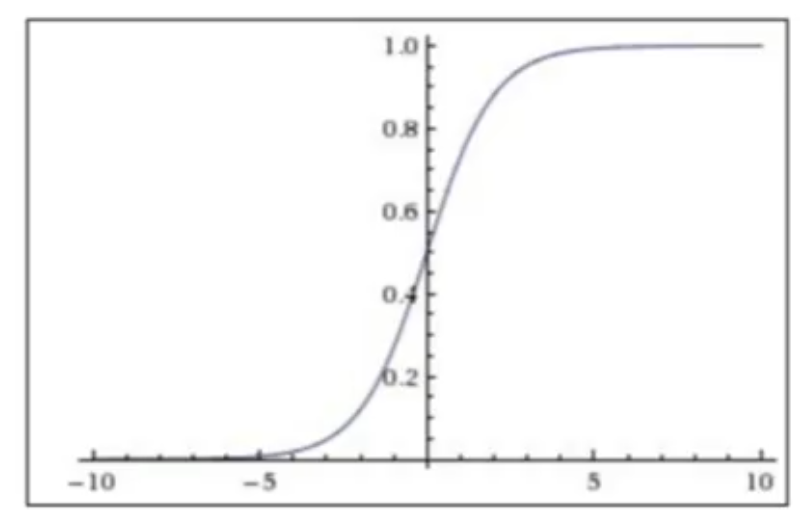
\includegraphics[width=0.5\columnwidth]{fei_fei_li/lecture_06/sigmoid.png}
tanh - $tanh(x)$ 

- Similar to sigmoid function
- the output is in the range of [-1,1]
- zero centered
- gradient = 0 when saturated

\paragraph{ReLU - $f(x) = max(0,x)$ }

- Rectified Linear Unit
- Does not saturate in the positive region
- Very computationally efficient
- Converges much faster than sigmoid and tanh (x6)
- More biologically plausible than sigmoid

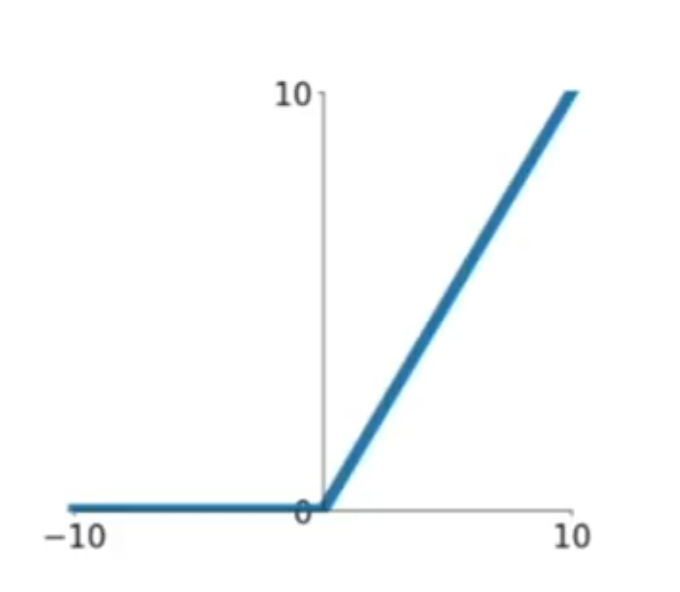
\includegraphics[width=0.5\columnwidth]{"fei_fei_li/lecture_06/Screenshot 2019-10-18 at 13.31.23.png"}

 Disadvantages

- does kill the gradient in the negative part of the regime
- It is possible to have dead ReLU that do not activate or update for a large part of the data. This can happen due to the following reasons:
  - bad initialization
  - learning rate is too high - large updates and the weights just around fast, the ReLU can get knocked off the data manifold

\paragraph{Leaky ReLU - $f(x) = max(0.01x, x)$ }

- Instead of being flat in the negative regime, it returns a negative gradient
- This solves the saturation problem and improves the convergence rate
- Computationally efficient

\paragraph{PReLU $f(x) = max(\alpha x, x)$}

- The $\alpha$ becomes another parameter
- Improves flexibility

\paragraph{Exponential Linear Unit (ELU)}

$$ f(x) = \begin{cases} x & \text{if} x > 0 \\ \alpha(exp(x)-1) & \text{if} x < 0 \end{cases}  $$ 

- expensive - requires an exponent
- this build back saturation in the negative regime 
- possible interpetation is that this is more robust to noise
- this is between relus and leaky ReLUs

\paragraph{Maxout $\max(w_1^Tx + b_1, w_2^T x + b_2)$}

- Generalization of ReLU and Leaky ReLU
- Linear regime 
- No saturation
- Doubles the number of parameters per neuron

\subsubsection{Guidelines to using activation functions }

- ReLU is the standard
- LReLU / Maxout / ELU are ok to try
- tanh can be used very carefully
- Don't use sigmoid :( original activation function - but people advanced to ReLU

\subsubsection{Data Processing Pipeline}

1. original data
2. zero - meaned data
3. normalized data - according to the std in each dimension
   - we need 0-mean data because any sort of bias will cause bias and (maybe) reduce the convergence

Approaches to normalize the data can include:

	- PCA - the data has diagonal covarriance matrix 
	- whitened data - the covariance matrix is identity
	- with images - stick to normalization, projecting pixel values into a lower dimensionality representation might not be beneficial
	- want to preserve spatial structure
	- training and test data are normalized in the same way
	- options include - subtract the mean image
	- subtract the per-channel mean

\subsubsection{Approaches to Initializing the NN:}

 - Setting initial nets - if all of the weights are 0 all of the neurons will respond in the same way, will all get the same gradient. 

 - Set initial weights to a small value that we sample from a normalized (Gaussian) with 0 mean W = 0.01*np.random.randn()
   	
   	- This works for small networks but does not work for deeper network
      	
      	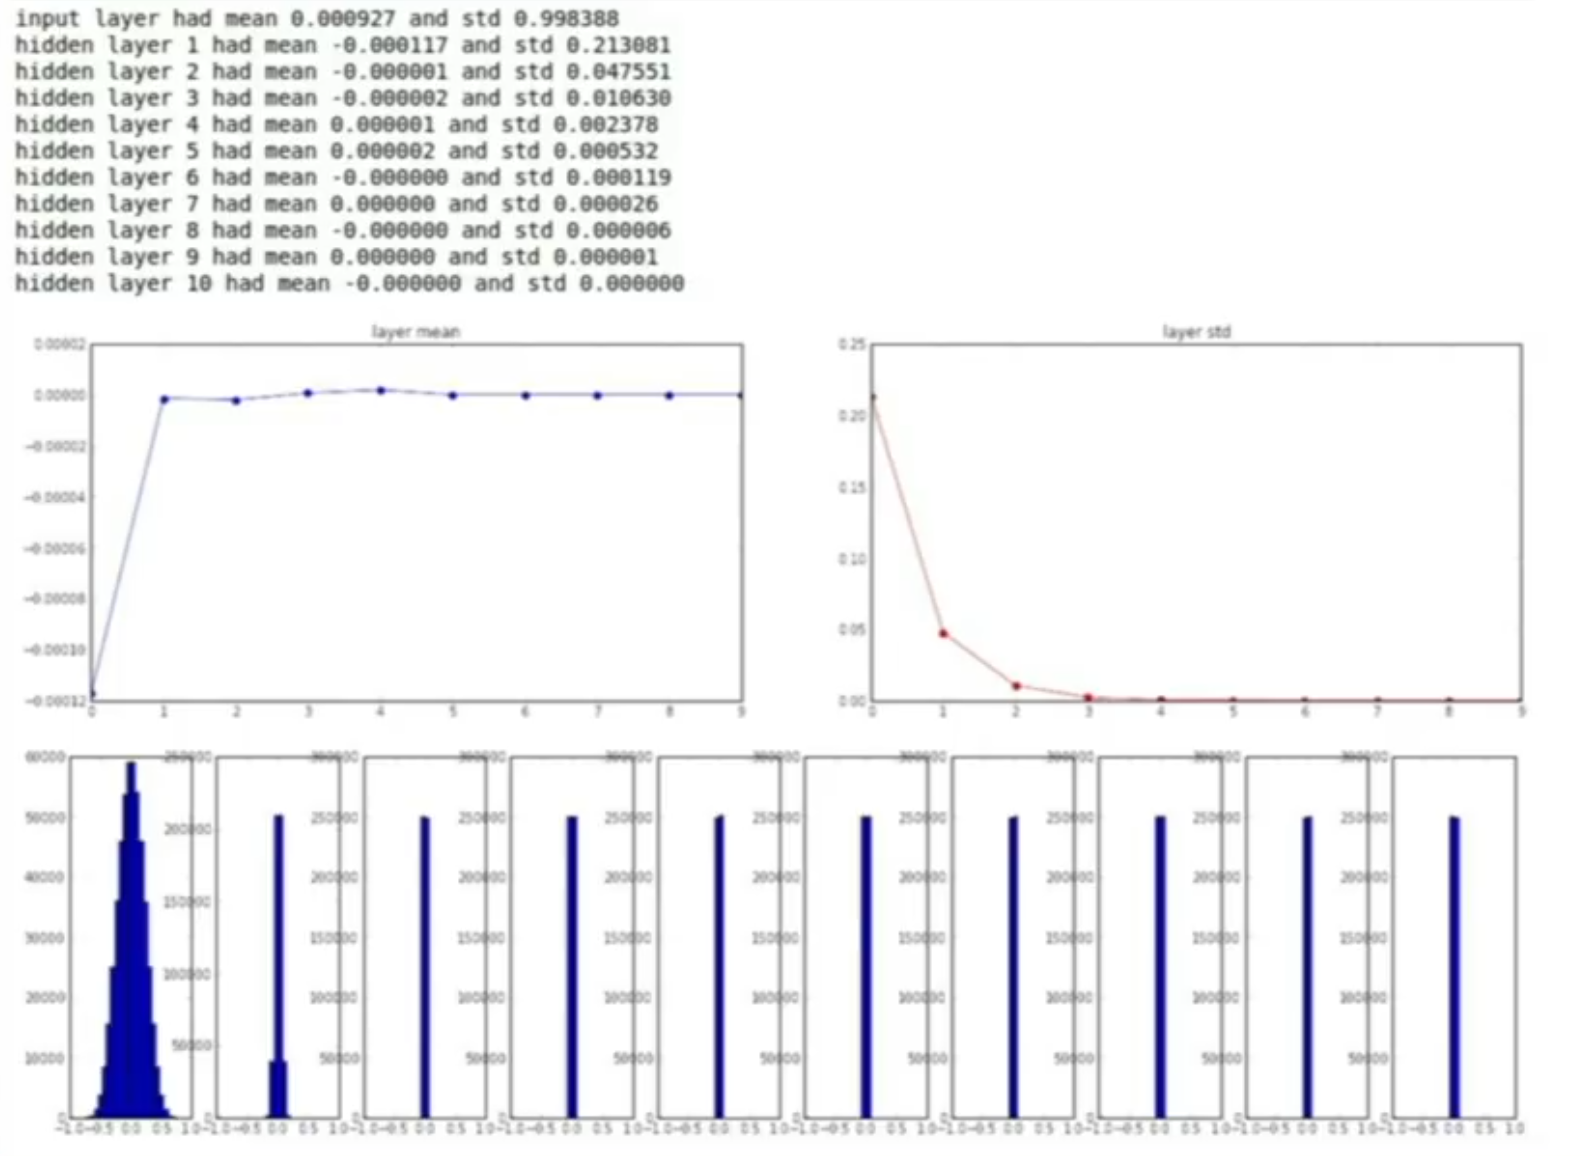
\includegraphics[width=0.5\columnwidth]{fei_fei_li/lecture_06/ecture_06_normalized-activation.png}
    
   - The mean for all of the layers is going to be zero which makes sense 

   - The STDEV shrinks at each layer and quicly collapses to 0 

 - Setting initial weights to large values - 
   	
   	
   
   - All of the neurons are going to be in the saturated regime, leading to values of $\pm1$ 
   
 - Xavier initialization - from Glorot
    - ${fan_{in}}$ - number of inputs
    - sample from a gaussian
    - normalize by the number of inputs
    - $W = random(min,max)/sqrt(min)$
    - variance of the input is equal to the variance of the outputs
       - small number of inputs - larger weights
       - large number of input - smaller weights
    
 - This reasonable initilization - math derivation assumes linear activation

 - But this breaks when you use a ReLU
   	
   	- the ReLU kills half of the neurons - sets the weights to 0 
    
   - changes the variance - so you can divide by 2 and this improves the weights

    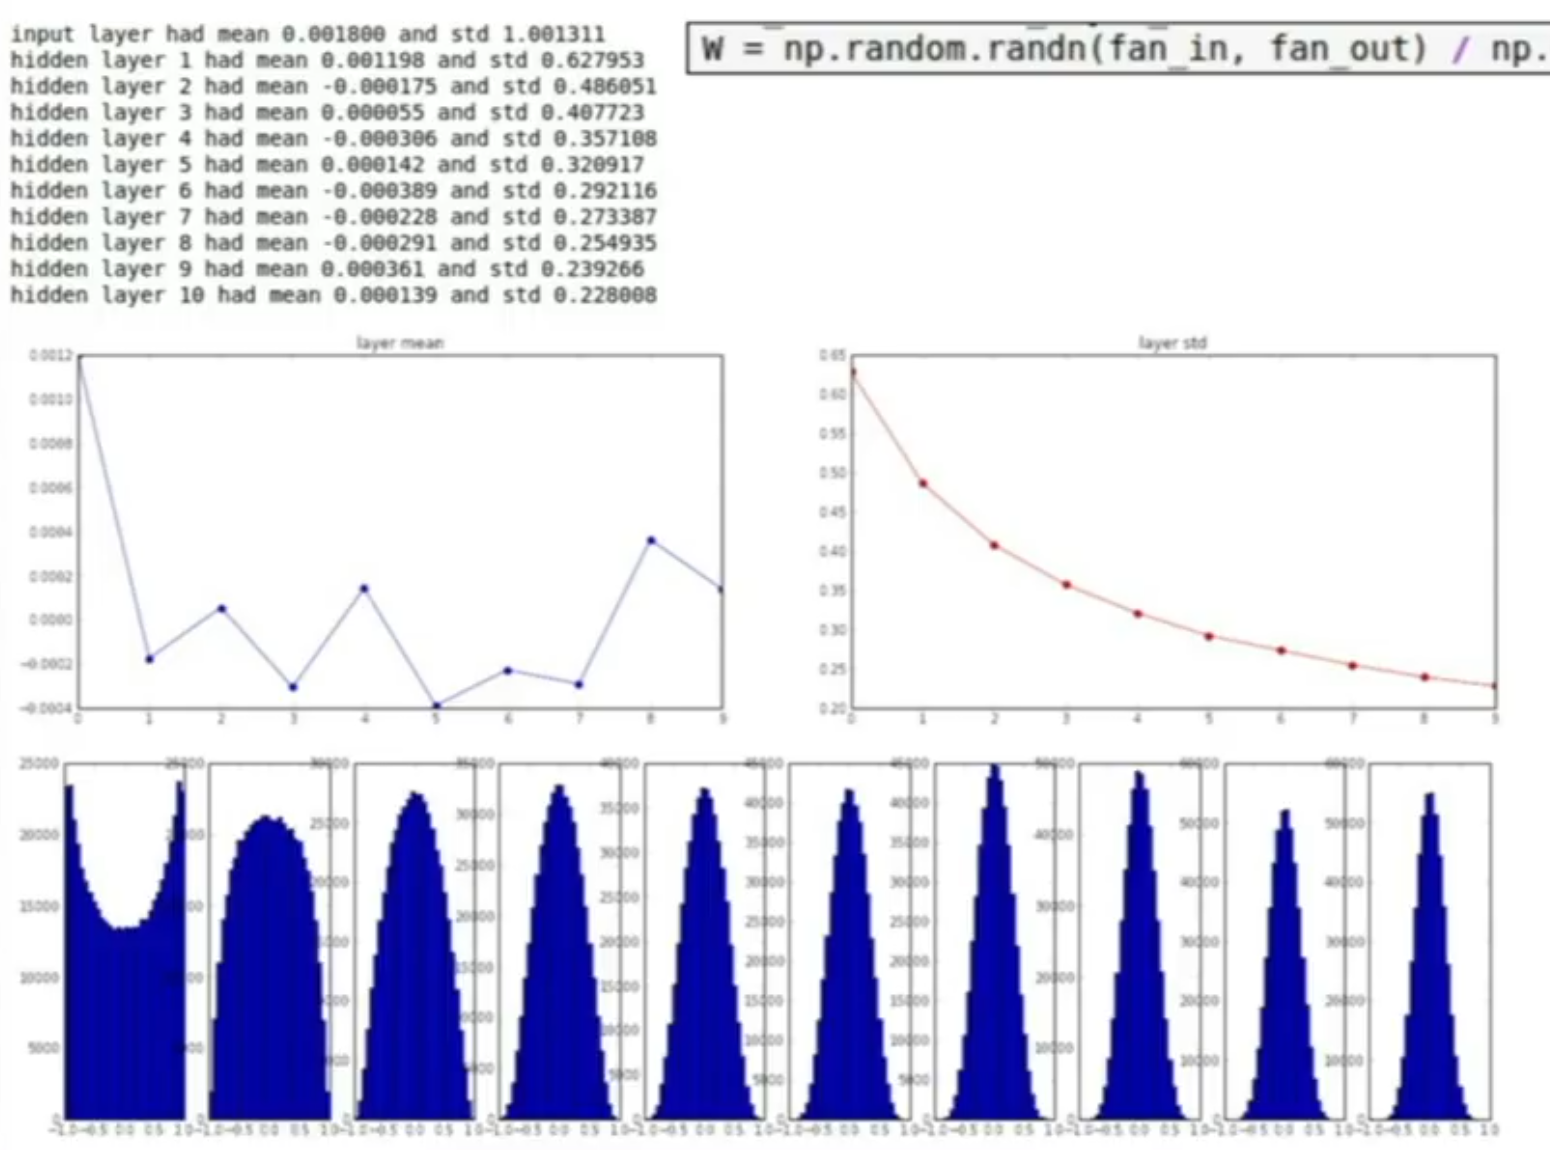
\includegraphics[width=0.5\columnwidth]{fei_fei_li/lecture_06/xavier_init_vis.png}

\subsubsection{Batch Normalization}

Consider a batch of activations at  some layer - make each dimension unit gaussian:

$$\hat x^k = \frac{x^{(k)} - E[x^{(k)}] }{\sqrt{\text{Var}[x^(k)]}} $$

which is differentiable

This is done per-dimension

The step is usually done after each fully connected layer and convolutional layers - to mitigate bad scaling effects at each layer

For convolutional layers - we also want to normalize jointly all spatial dimensions and all of the training examples - i.e. we want nearby locations to be normalized in the same way - one mean and one stdev for one actibation map we have. 

Check out **Ioffe and Szegedy, 2015** and understand the paper and the methods they present. 

We might not necc. want unit Gaussian input to the tanh layers: this constraints you the linear regime of the non-linearity.



We can add a scaling and shifting operation - but the network can learn a scaling $\gamma = \sqrt{Var(x)}, \beta = E[x^k]$ which is the identity mapping

$y^{(k)} = \gamma^{(k)}\hat{x}^k + \beta^{(k)} $

Improves gradient flow through the network 

More robust - higher learning rates and diff. init.

Regularization - each of the outputs is dependent on the inputs as well as the outputs of all images in the batch



At test time the batch norm functions differently: a single fixed mean of activation during training is used (can be estimated during training with running averages)

\subsubsection{Monitoring Training }

1. Preprocess the data

2. Choose the architecture

   1. input - hidden layer - output

3. Validation - step 1 - ensure loss is reasonable 

   1. disable regularization
   2. do a forward pass
   3. test the loss is reasonable
   4. for example for softmax the "correct" loss is about -log likelihood

4. Regularization validation

   1. add reg. 
   2. observe the loss increases

5. Validate arch works:

   1. start with a very small set of data
      - small set - be able to fit the data very well.
      - turn off reg
      - use simple vanilla sigmoid
   2. ensure that the loss can go down to 0 and training accuracy goes up to 1

6. Figure out the training rate (step size):

   - start with small regularization and find the learning rate to make the loss go down
   - in early stages of learning with softmax, even though the loss does not change much, we can observe large jumps in accuracy because small shifts in labels can lead to large changes to the classification with softmax
   - NaN - learning rate too high
   - A good range [1e-3, 1e-5]

7. Hyperparameter Optimization

   Cross validation in stages, coarse to fine

   Best to optimize in log space

   - Stage 1:
     - try a few epoch instances
     - pick values spread out apart
   - Stage 2:
     - longer running time, finer search
   - Solver explosion detection: 
     - if the cost is x3 original cost, quit
   - If all learning rates are at the edge of our hyperparameter sampling space, it means we might not have explored the range appropriately
   - Random Search vs. Grid Search (Begstra and Bengio, 2012)
     - Grid layouts 
     - Better to sample randomly from each parameters in the range
     - If a function is dependent more on one variable than another, which is usually true, because we have lower effective dimensionality than what we usually have, we will have more samples of the important factor - more useful signal
   - Hyperparameters:
     - network arch.
     - learning rate, decay schedule, update type
     - regularization (l2/dropout)

8. Bad Init - flat learning curve

9. Track ratio of weight update / weight magnitude - ratio of 0.01-0.001 is about good

\paragraph{Training a Neural Network}

1. Randomly initialize the weights
2. Implement forward propagation to get $h_\theta(x(i))$  for any $x^{(i)}$
3. Implement the cost function
4. Implement backpropagation to compute partial derivatives
5. Use gradient checking to confirm that your backpropagation works. Then disable gradient checking.
6. Use gradient descent or a built-in optimization function to minimize the cost function with the weights in theta.

\subsubsection{Stochastic Gradient Descent}

Normal gradient descent:

\begin{verbatim}
while True:
  weights-grad = evaluate_gradient(loss-fun, data, weights)
  weights += - step-size * weights-grad
\end{verbatim}


High condition number - cases of functions where the loss changes quickly in one direction and slowly in another direction. The ratio of the smallest to the largest singular value in the Hessian matrix

For functions such as this, there's a tendency to zig zag (valley problem), leading to slow convergence. This problem is more common in higher dimensions.

Local minima and saddle points:

SGD will get stuck because the gradient is 0.

Saddle points are common in high dimensions. The problem is also close to the saddle point.

Stochastic - the gradient and loss are estimated using a small number of example batches

Any noise in the gradient means that the optimization wanders around in the space and might take a lot of time to converge

Momentum term:

We step in the direction of our velocity and add friction

This simple strategy helps a lot.

Nesterov Estimated Gradient: 

Evaluate the gradient at the point where the velocity vector takes you, and mix the two to step again from the original point

tendency to overshoot minimum, nesterov tends to overshoot less.

flat minima are prob. generalizing better - recent theoretical work

feature, not a bug that sgd momentum skips over sharp minima

\paragraph{AdaGrad}

\begin{verbatim}
grad_squared = 0
while True:
  dx = compute-gradient(x)
  grad_squared += dx * dx 
  x -= learning_rate * dx / np.sqrt(grad_squared) + 1e-7)
\end{verbatim}

What it does: 

1. normalizes the relative step size in each dimension based on the history, so it will increase step size for variable with small gradient and dec step size for variables with high gradient
2. Over time the step size decays - in the convex case it is good. non convex case, it is problematic - you might get stuck with adagrad

\paragraph{RMSProp}
\begin{verbatim}
grad_squared = 0

while True:
  dx = compute_gradient(x)
  grad_squared += decay_rate*grad_squared + (1 - decay rate) * dx * dx
  x -= learning_rate * dx / np.sqrt(grad_squared) + 1e-7)
\end{verbatim}

0.9 or 0.99 decay rate.

estimates are leaky - not always slowing down?

RMS prob does not tend to overshoot as much, the optimization makes equal progress along all dimensions

AdaGrad decays quickly if the learning rate is fixed relative to other methods.

\paragraph{Adam}

Maintain an estimate of the first and second moment

Momentum

Bias correction

AdaGrad/RMSProp

If the valley problem is not xis aligned, non of the algorithms can deal with that (think squished taco)



let's compare Adam and AdaGrad/RMSProp with momentum:

\begin{verbatim}
first_moment = 0
second_moment = 0

while True:
  dx = compute_gradient(x)
  first_moment = beta1 * first_moment(1-beta1)              //momentum
  second_moment = beta2 * second_moment(1-beta1)*dx         //AdaGrad/RMSProp
  x -= learning_rate * first_moment / (np.sqrt(second_moment) + 1e-7 )  
\end{verbatim}

% \begin{verbatim}
% first_moment = 0
% second_moment = 0

% while True:
% ​	dx = compute_gradient(x)
% ​	first_moment = beta1 * first_moment(1-beta1)   						//momentum
% ​	second_moment = beta2 * second_moment(1-beta1)*dx					//AdaGrad/RMSProp
% ​	x -= learning_rate * first_moment / (np.sqrt(second_moment) + 1e-7 )	
% \end{verbatim}

And in fact full form Adam is: 

\begin{verbatim}
first_moment = 0 
second_moment = 0

for t in range(num_iterations):
  dx = compute_gradient(x)
  first_moment = beta1 * first_moment(1-beta1)   						//momentum

  second_moment = beta2 * second_moment(1-beta1)*dx					//AdaGrad/RMSProp
  first_unbias = first_momentum / ( 1 - beta1 ** t)
  second_unbias = second_momentum / ( 1 - beta2 ** t)
  x -= learning_rate * first_unbias / (np.sqrt(second_unbias) + 1e-7 )
\end{verbatim}


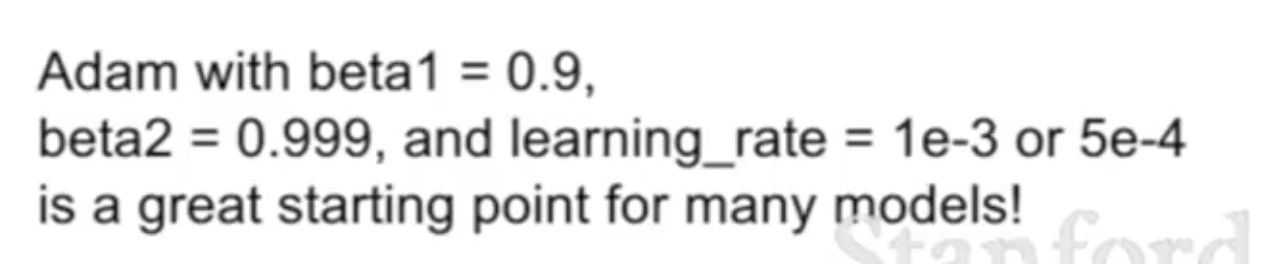
\includegraphics[width=0.5\columnwidth]{fei_fei_li/lecture_07/adam_params.png}

\paragraph{Learning Rate Decay}

Step decay - half the learning rate every few epochs

exponential decay - $\alpha = \alpha_0e^{-kt}$ 

1/t decay - $\alpha = \alpha / (1+kt) $ 

More Common with SGD and Momentum and less common with Adam

Start without learning rate decay

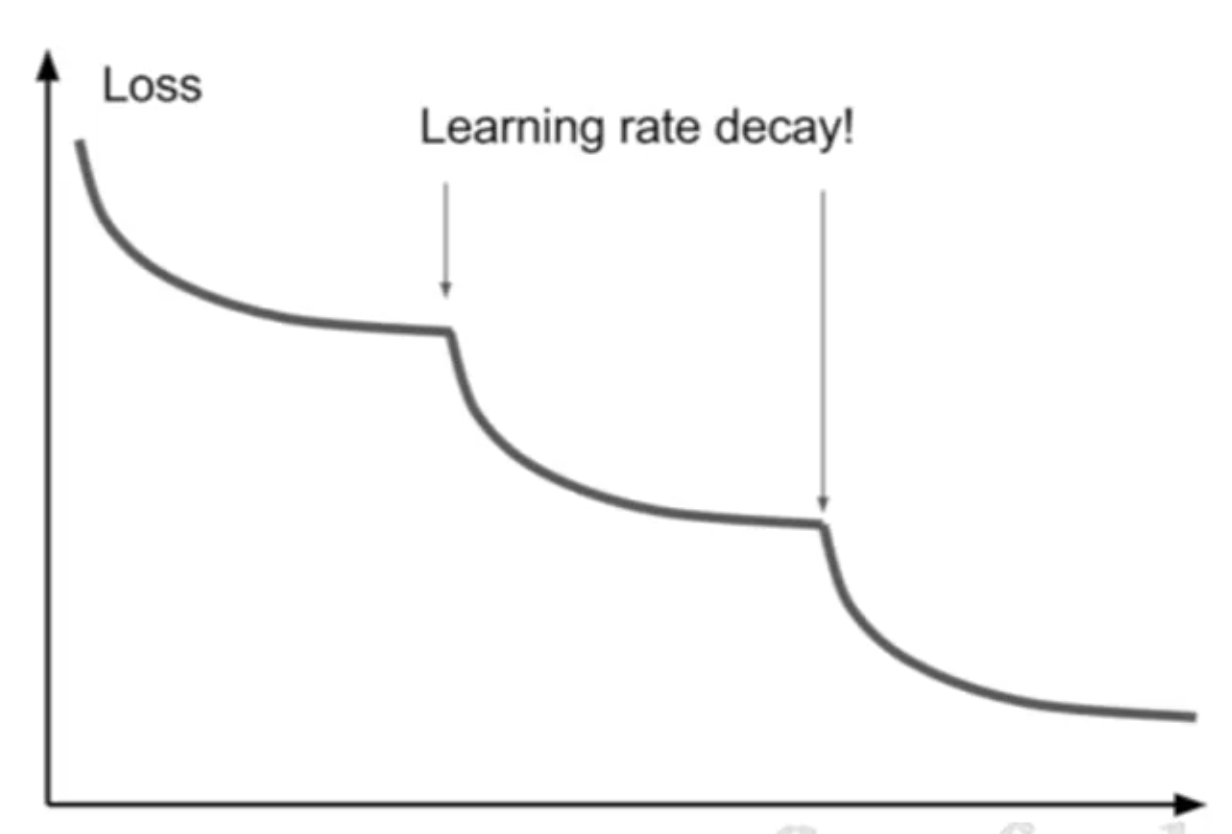
\includegraphics[width=0.5\columnwidth]{fei_fei_li/lecture_07/learning_rate_decay.png}

All of these algorithms are **First Order Optimization Algorithms**

1. Use gradient to approximate the derivative (in a linear manner)
2. Step to minimize approximation

The step does not hold for large step size

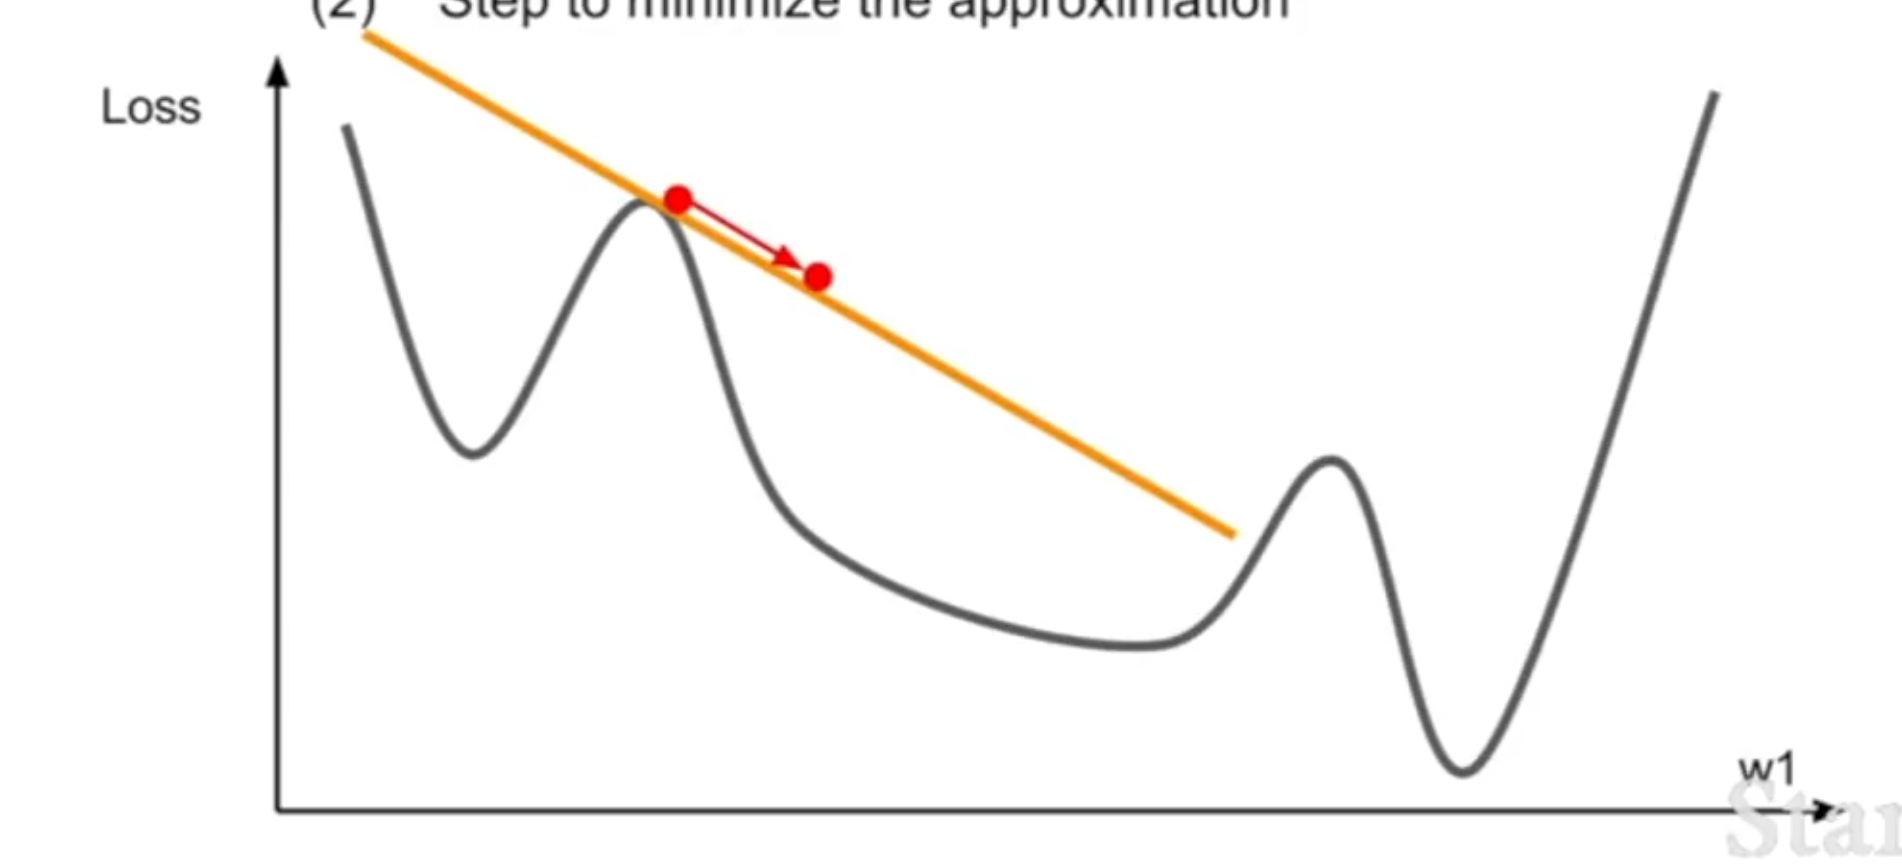
\includegraphics[width=0.5\columnwidth]{fei_fei_li/lecture_07/first_order_approx.png}

\paragraph{Second order approximation}

We can use a second order approx. of the gradient incorporating the Hessian

We can then step to the minimum of the approximated function

This is called the Newton step - it does not have a learning Rate!

This is impractical for deep learning, Hessian is $O(N^2)$ which can be a few millions

cannot invert or store in memory

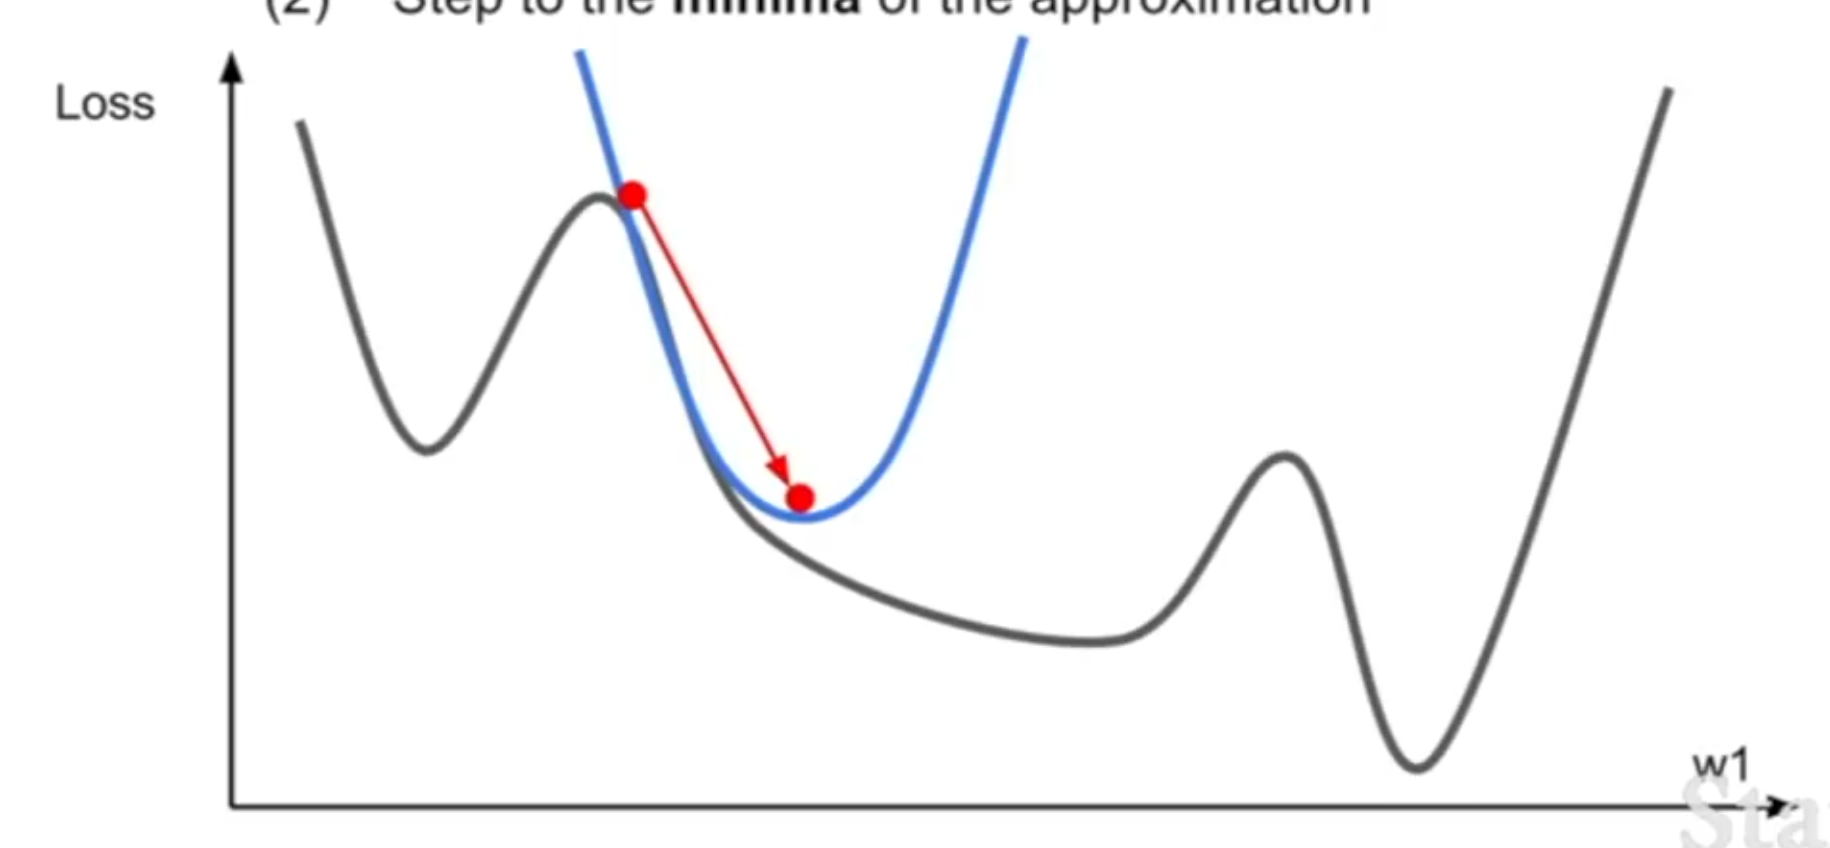
\includegraphics[width=0.5\columnwidth]{fei_fei_li/lecture_07/second_order_approx.png}

Alternative are BFGS and L-BFGS which are approximations of the Hessian

L-BFGS works well for full batch deterministic 

Doesn't work very well for mini-batches, the approximations do not handle the stochastic case too well. In practice counter this by:

- Adam
- If you can afford full batch, LBFGS

Until now all of this was about training error. But we can more about test data, and reducing the gap on test data! So, what can we do? 

\paragraph{Model Ensemble}

1. Train multiple independent models
2. Test time average their results - 2% extra performance
3. Consistent improvement - used often in benchmarks
4. Also keep snapshots of the model during training
5. Polyak averaging - save some running average of the model parameters

\subsubsection{Regularization}

Regularize the model to have it generalize better from training to test data

L2 Regularization - $R(W) = \sum_k\sum_lW_{k,l}^2 $

L1 Regularization - $R(W) = \sum_k\sum_l | W_{k,l} |$

Elastic net - $R(W) = \sum_k \sum_l \beta W^2_{k,l} + | W_{k,l} |$

In practice this regularization doesn't make  too much sense in NN.

\paragraph{	Dropout }

At every forward pass through the network, randomly set some neurons to 0

The probability is a hyper-parameter, usually set to 0.5

More common for fully connected layers, but sometime to might drop channels in conv layers

Dropout means  the network cannot rely on a single feature too much

Similar to doing a model ensemble within a single model

Dropout affects the expected value of our variable - (i didn't get  the full idea of this and it is used in test time) - but at test time we multiply by the dropout probability

For a single neuron with two inputs:

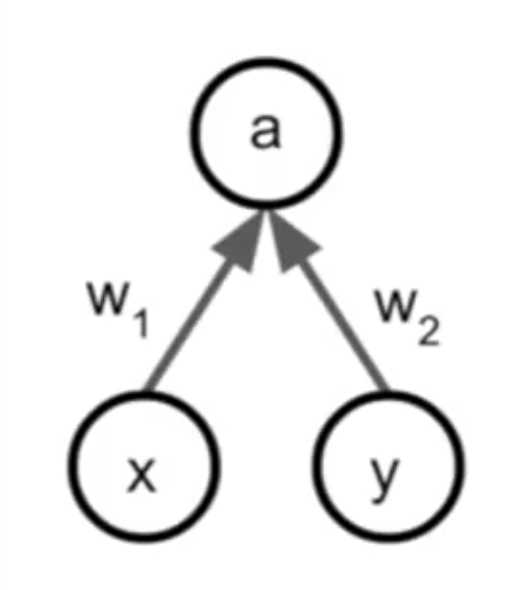
\includegraphics[width=0.5\columnwidth]{fei_fei_li/lecture_07/Screenshot 2019-10-21 at 11.32.00.png}

Train: $E[a] = \frac{1}{4}(w_1x+w_2y)+\frac{1}{4}(w_1x+0y)+\frac{1}{4}(0w_1x+w_2y)+\frac{1}{4}(0x+0y) = \frac{1}{2}(w_1x+w_2y)$

Test: $E[a] = w_1x+w_2y$

At test time - multiply by dropout probability

\paragraph{Inverted Dropout}

You divide by $p$ during training time, rather than multiply by $p$ during test time

Training with dropout takes longer to train, but better generalization after in converged.

A different look at this: 

Training - add randomness

Test - average out randomness

Batch normalization is similar - stochastic relative to a single data point

But dropout gives you control on the amount of randomness vs. batch normalization

\paragraph{Data Augmentation}

- Random image transformation - mirror, cropping
  Resize image at 5 scales
  Report performance at a single crop and at five standard crops

- Color jittering
  Possible in some data dependent way

- Basically - how we can change the data without the label

\paragraph{Drop Connect}

Randomly 0 out the weights

\paragraph{Fractional Max Pooling}

Randomize the regions over which we pool

\subsubsection{Transfer Learning}

For example, want to use learning from a general network to a more specific network which can label 10 dog breeds from a smaller dataset

Cafe etc are 

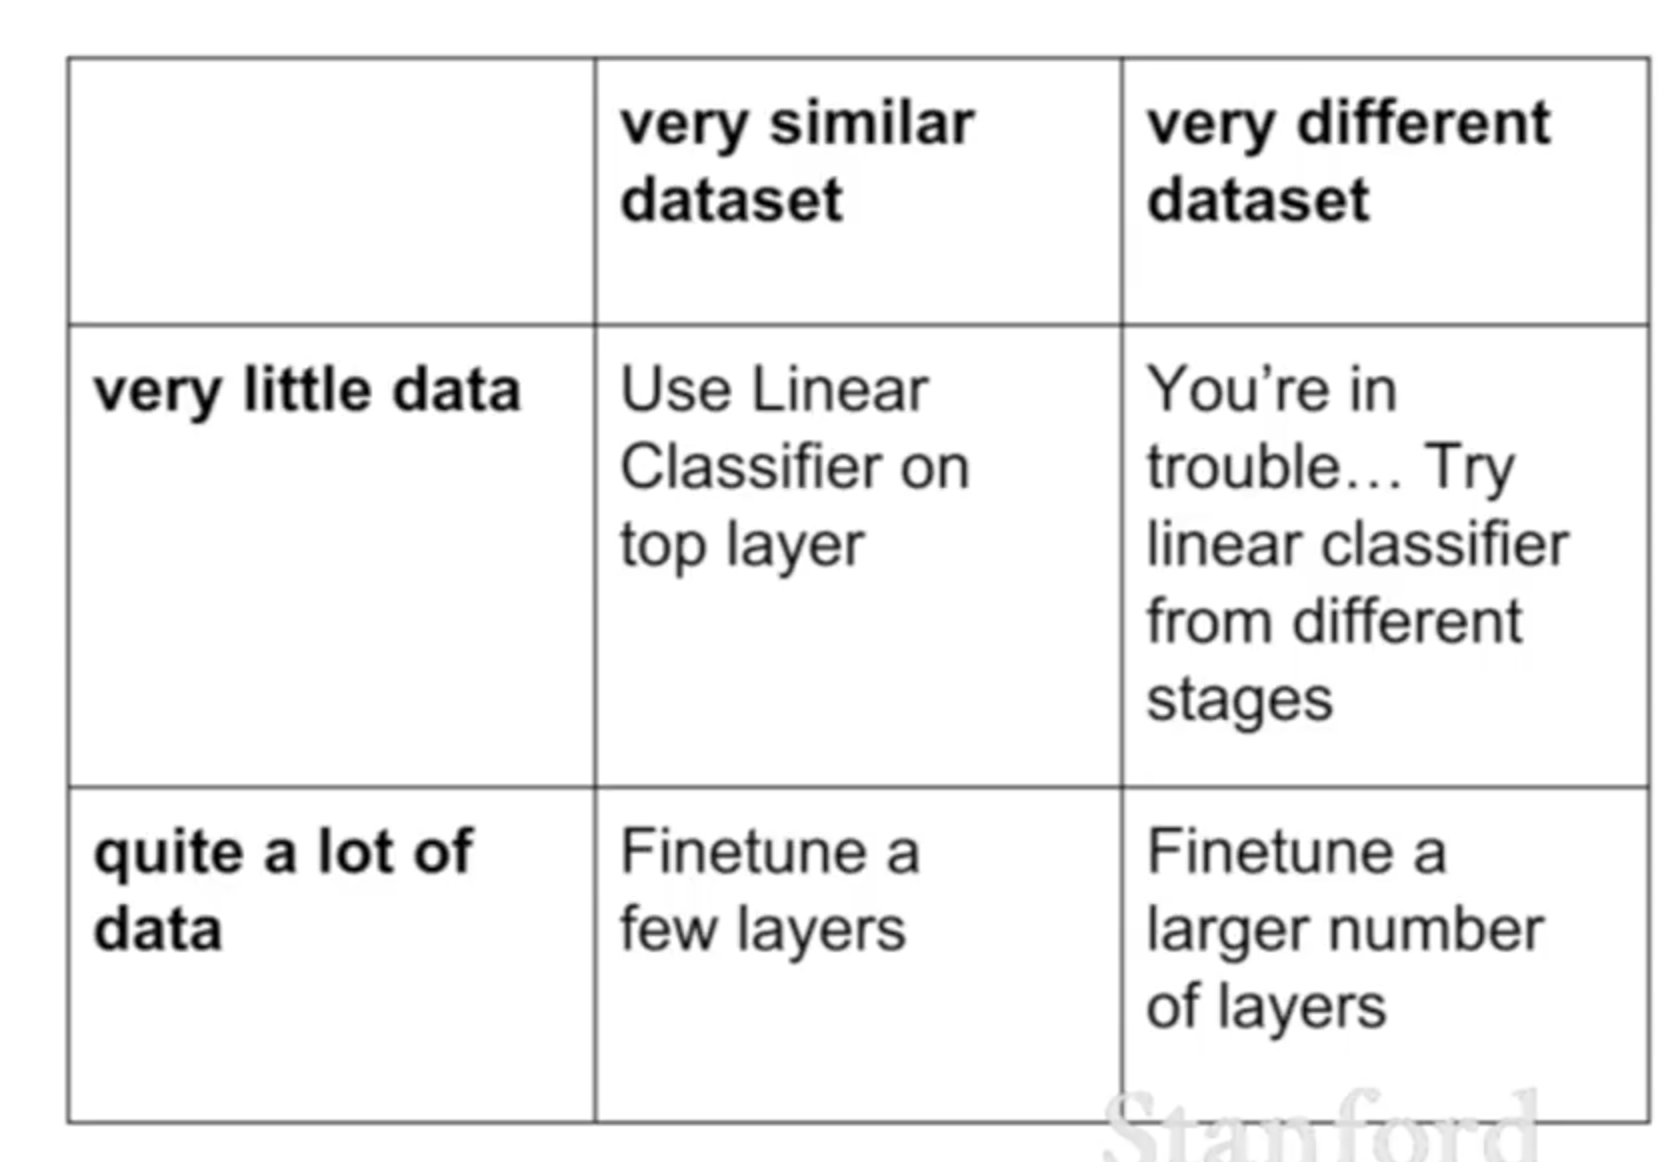
\includegraphics[width=0.5\columnwidth]{fei_fei_li/lecture_07/guidelines_transfer_learning.png}

\subsection{Deep Learning Software}

\subsubsection{CPU vs. GPU}

GPU cores have 3840 units vs. 20 threads running on CPUs 

But they run at lower clock speed, simpler operations

Parallelize one task across many cores

Good for performing a similar task

GPU CPU communication is a bottle neck

12GB memory is the max atm (2017) on GPU memory + caching hierarchy

Matrix multiplications are very suitable on GPU

Benchmarks show 60-70x performance gain

x3 performance gain by using optimized CUDA implementations - use cuDNN

Another problem - model is on GPU and the data is on SSD

this adds a bottle neck - solutions:

	- read data in RAM
	- use SSD
	- multiple CPU threads to pre-fetch data
	- 

\subsubsection{TensorFlow}

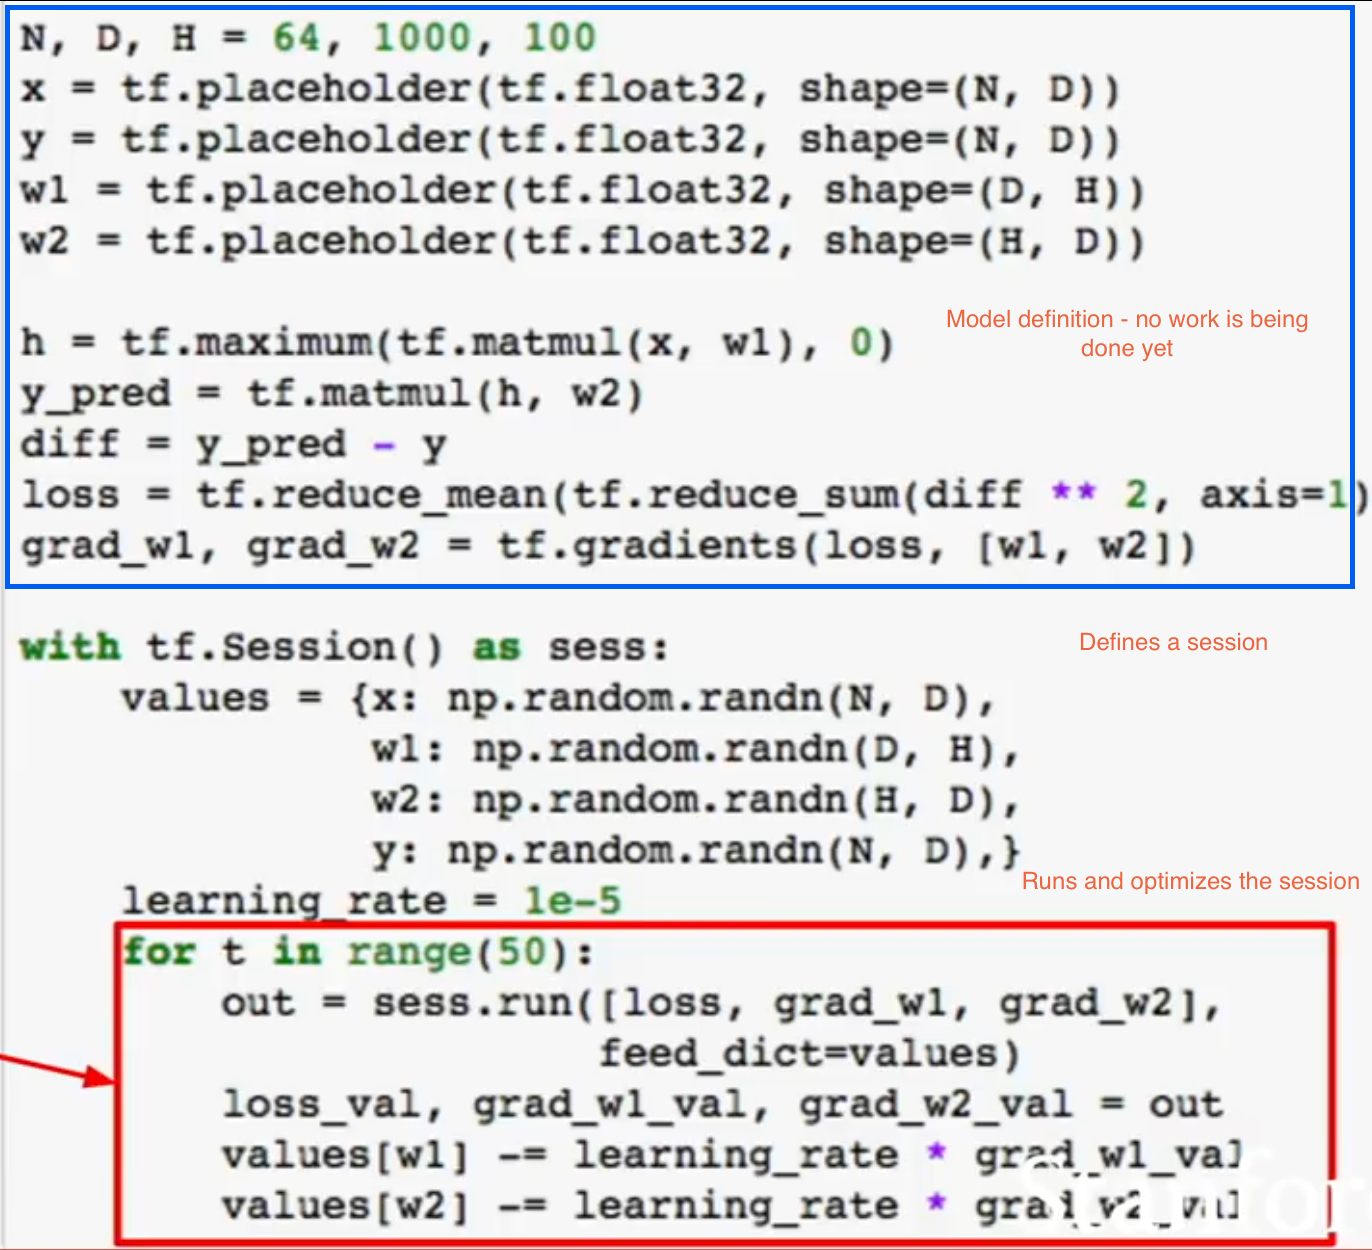
\includegraphics[width=0.5\columnwidth]{fei_fei_li/lecture_08/Screenshot 2019-10-21 at 12.32.42.png}

Where it's done like this - every time we run the graph we're copying the weights from numpy arrays to memory, etc. very expensive.

The solution is to setup w1 and w2 as tf.Variable - lives inside the computational graph and we also need to tell TF how to initialize them

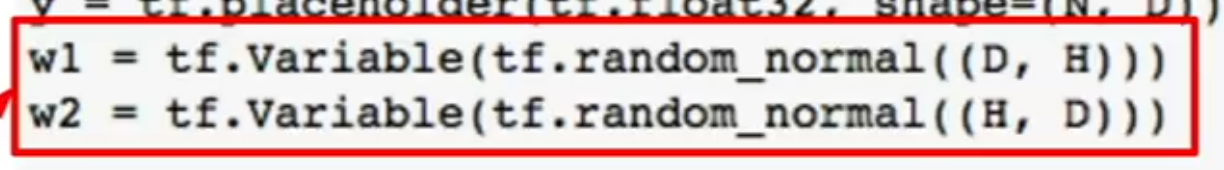
\includegraphics[width=0.5\columnwidth]{"fei_fei_li/lecture_08/Screenshot 2019-10-21 at 12.45.00.png"}

So in this version the weights update step needs to live within the computational graph, so the final version is this? 

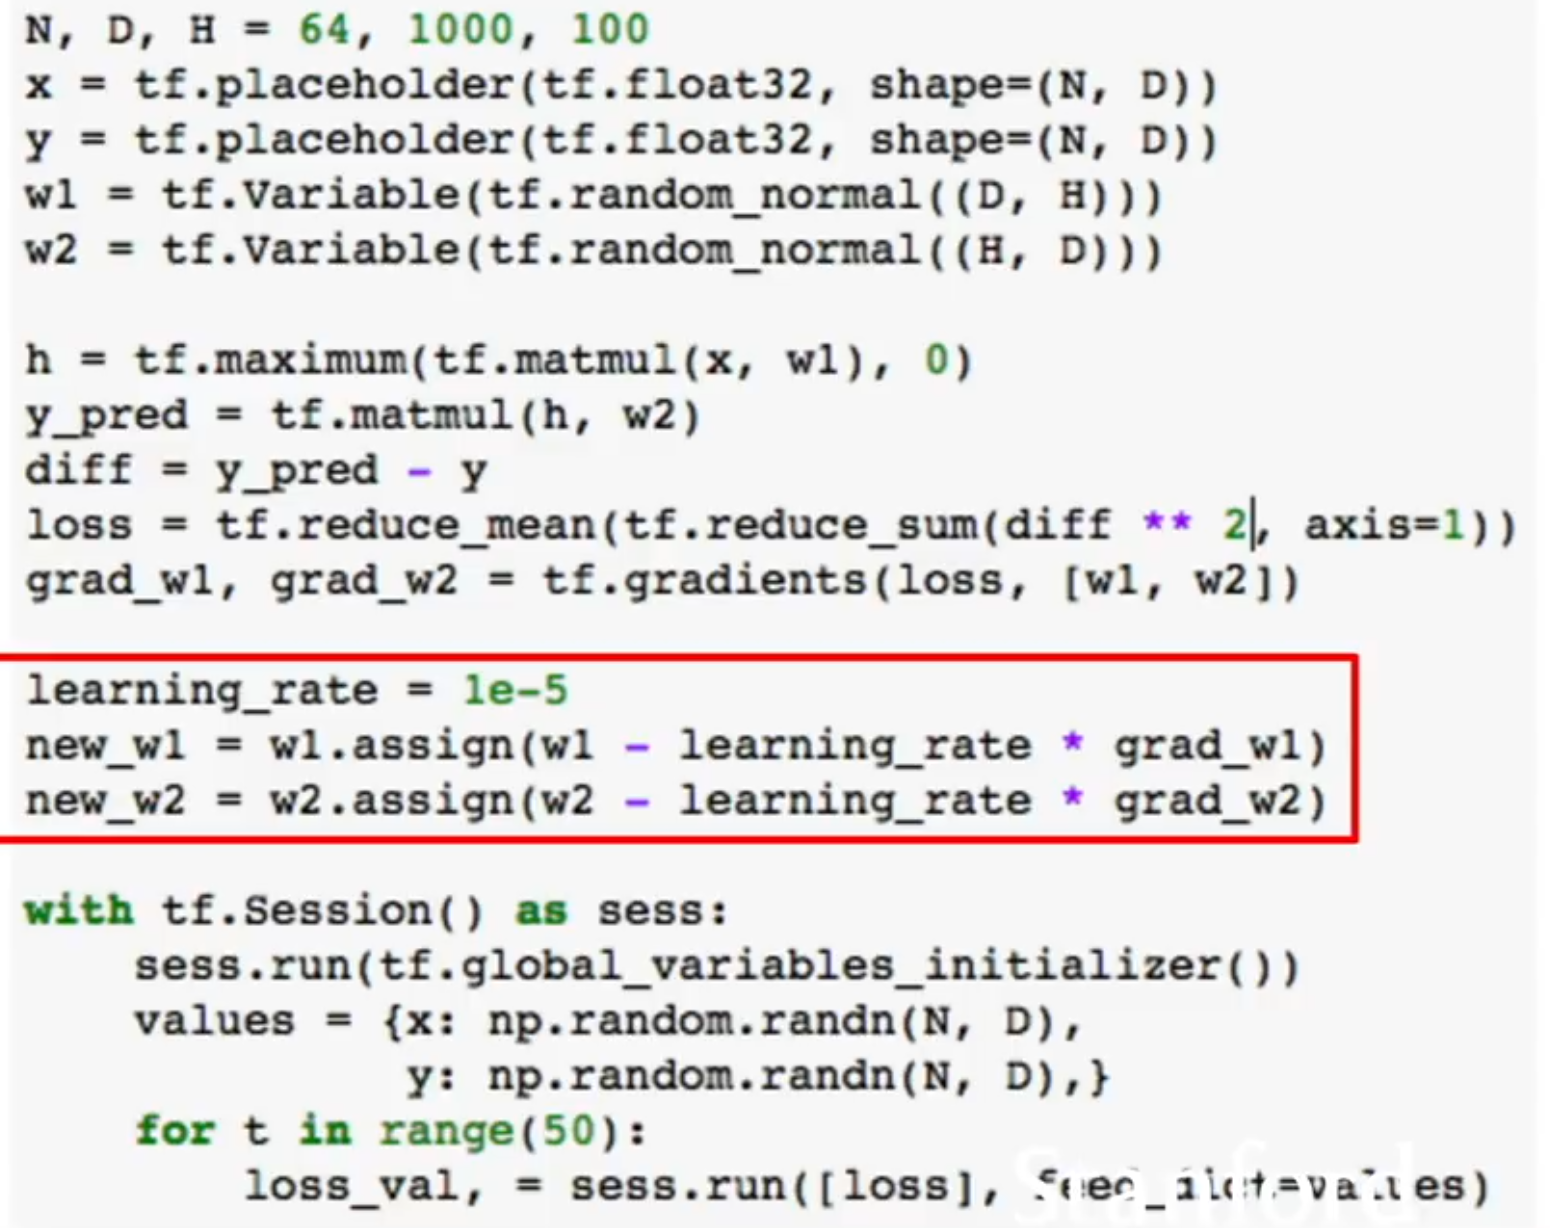
\includegraphics[width=0.5\columnwidth]{fei_fei_li/lecture_08/tf_in_memory.png}

so we have to add a dummy node which is responsible for updating the weights:

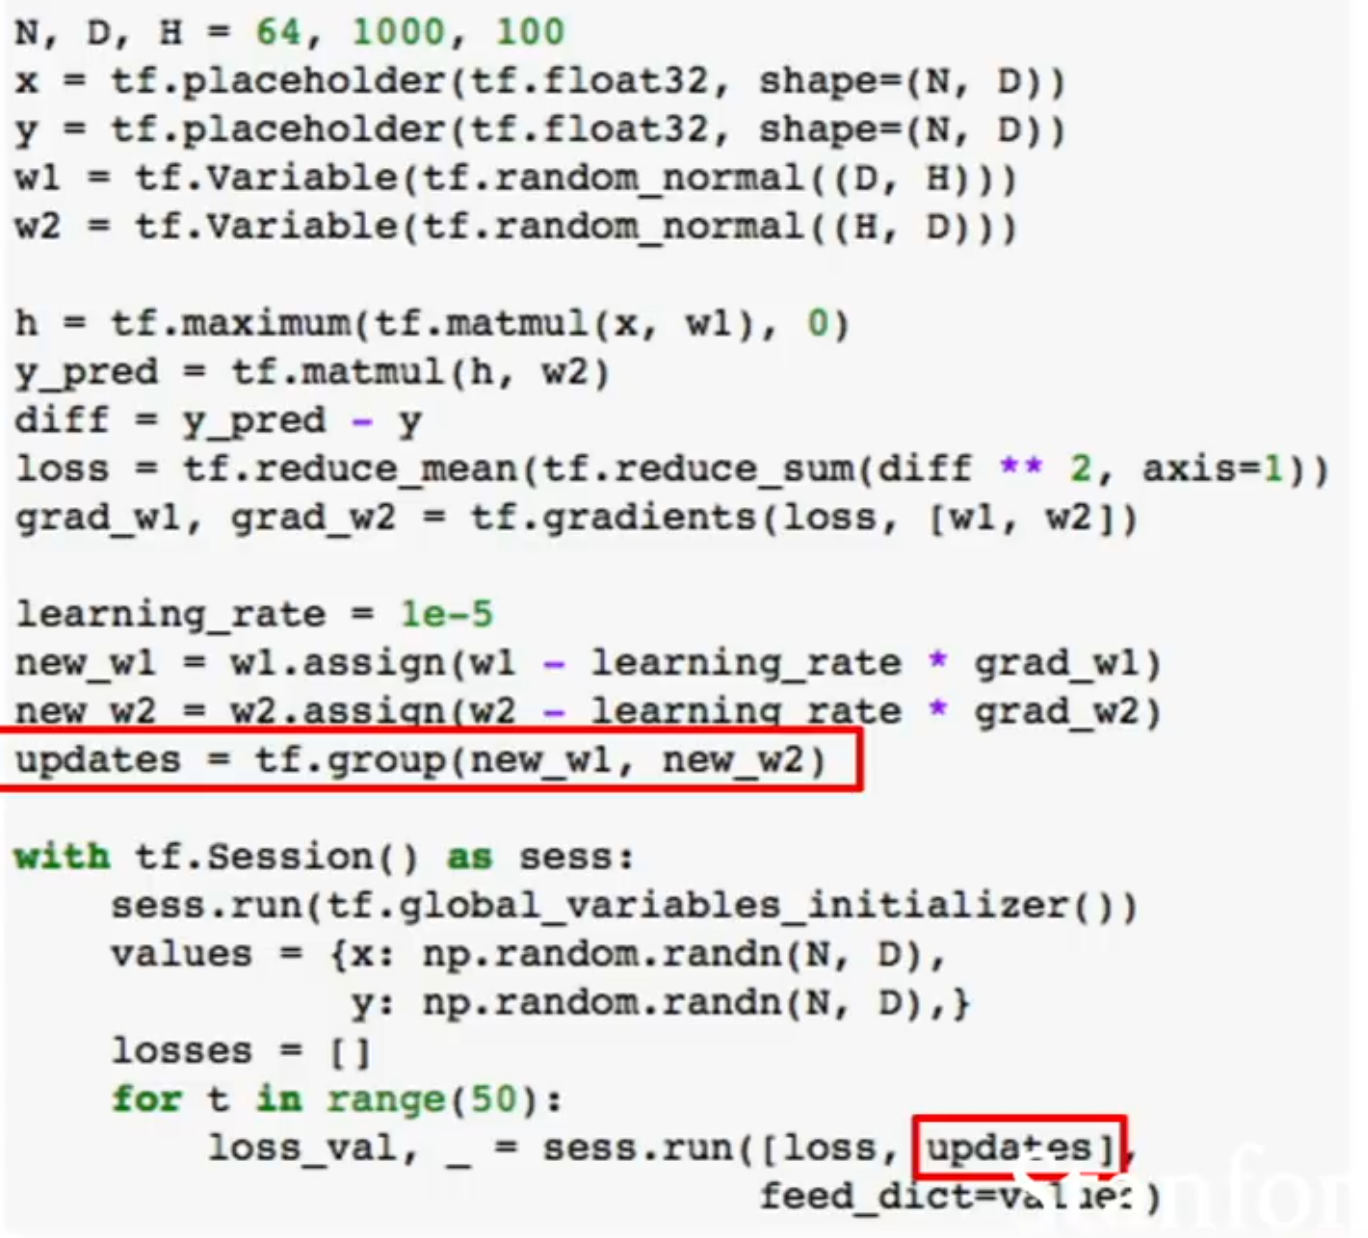
\includegraphics[width=0.5\columnwidth]{fei_fei_li/lecture_08/tf_memory_updates.png}

and tell tf to update the node.

This is a bit ugly, we can simple use an TF optimizer: 

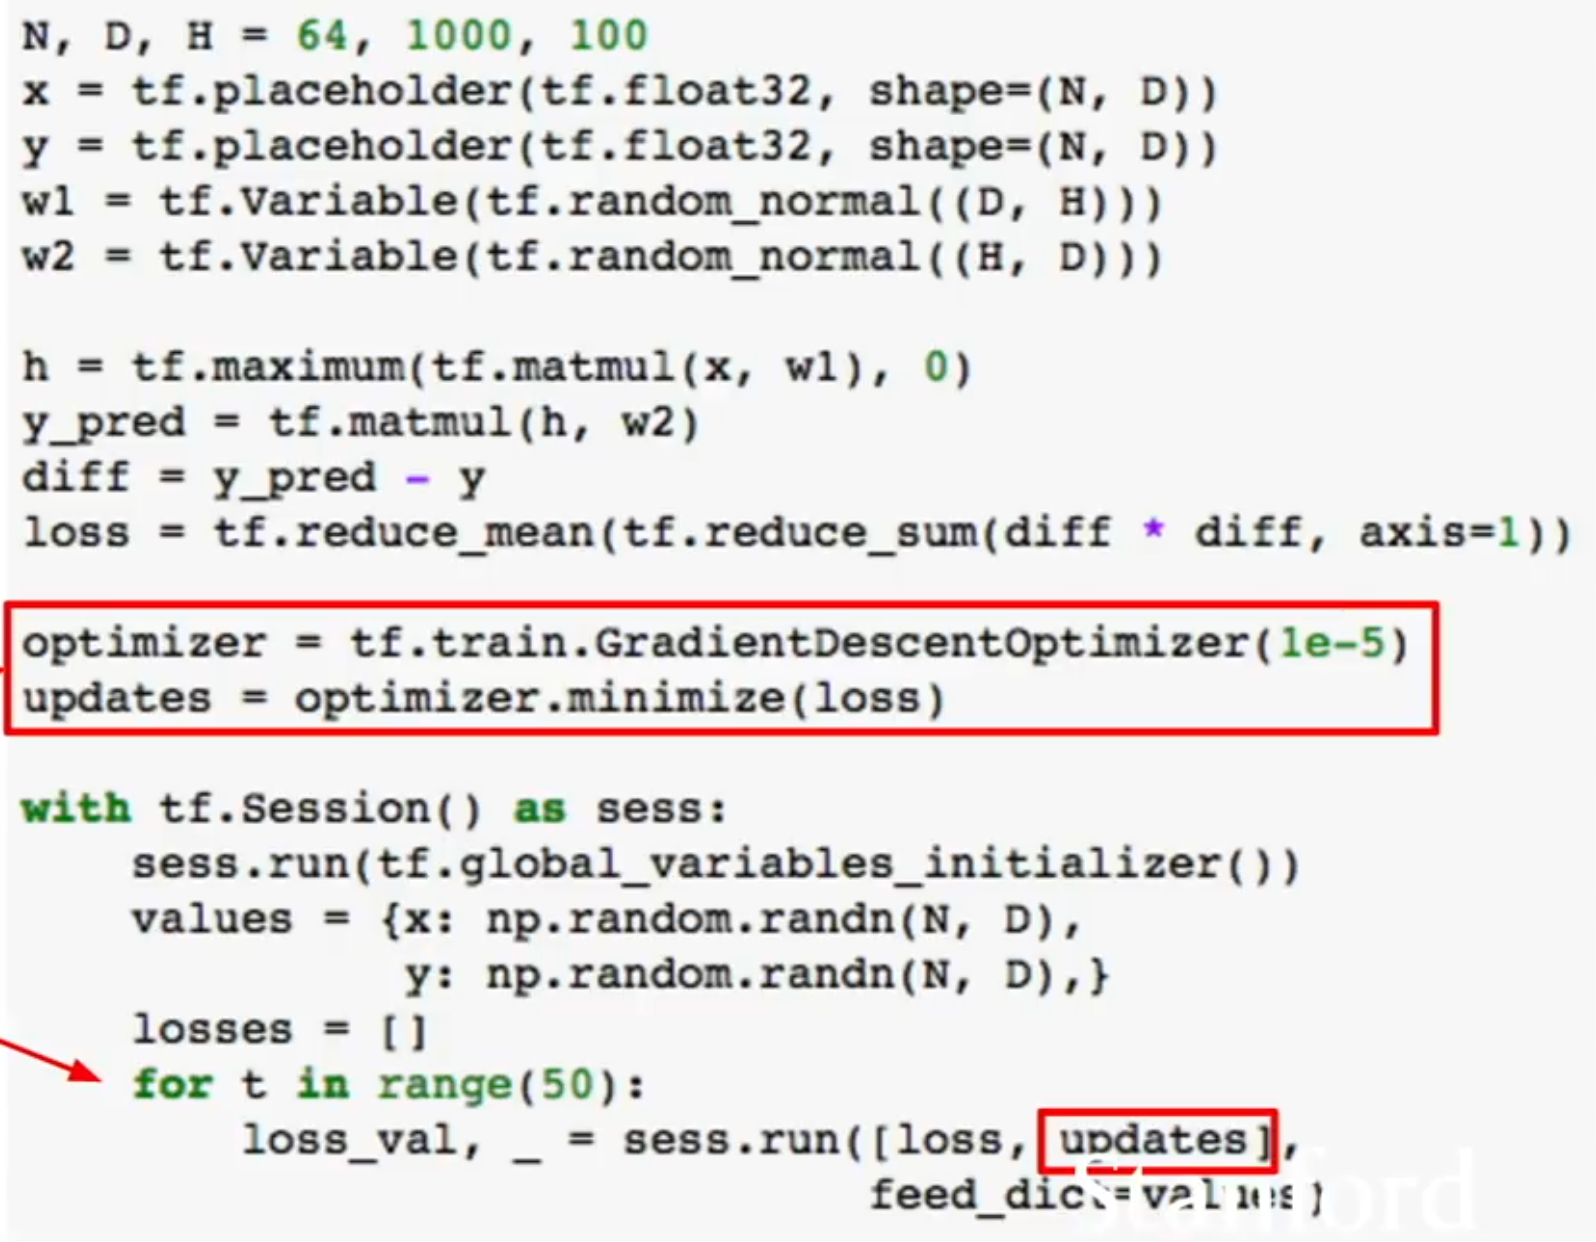
\includegraphics[width=0.5\columnwidth]{fei_fei_li/lecture_08/optimizer.png}

which adds the relevant nodes to the graph (compute gradients, update weight, group operations)

\subsubsection{PyTorch}

Has 3 different levels of abstraction

- tensor - imperative ndarray on gpu
- variable - node in a comp. graph
  - support automatic diff
  - same API as tensors
  - flagged if we want to compute gradients
- module - nn layer, may store state and learnable weights



\paragraph{tensors}

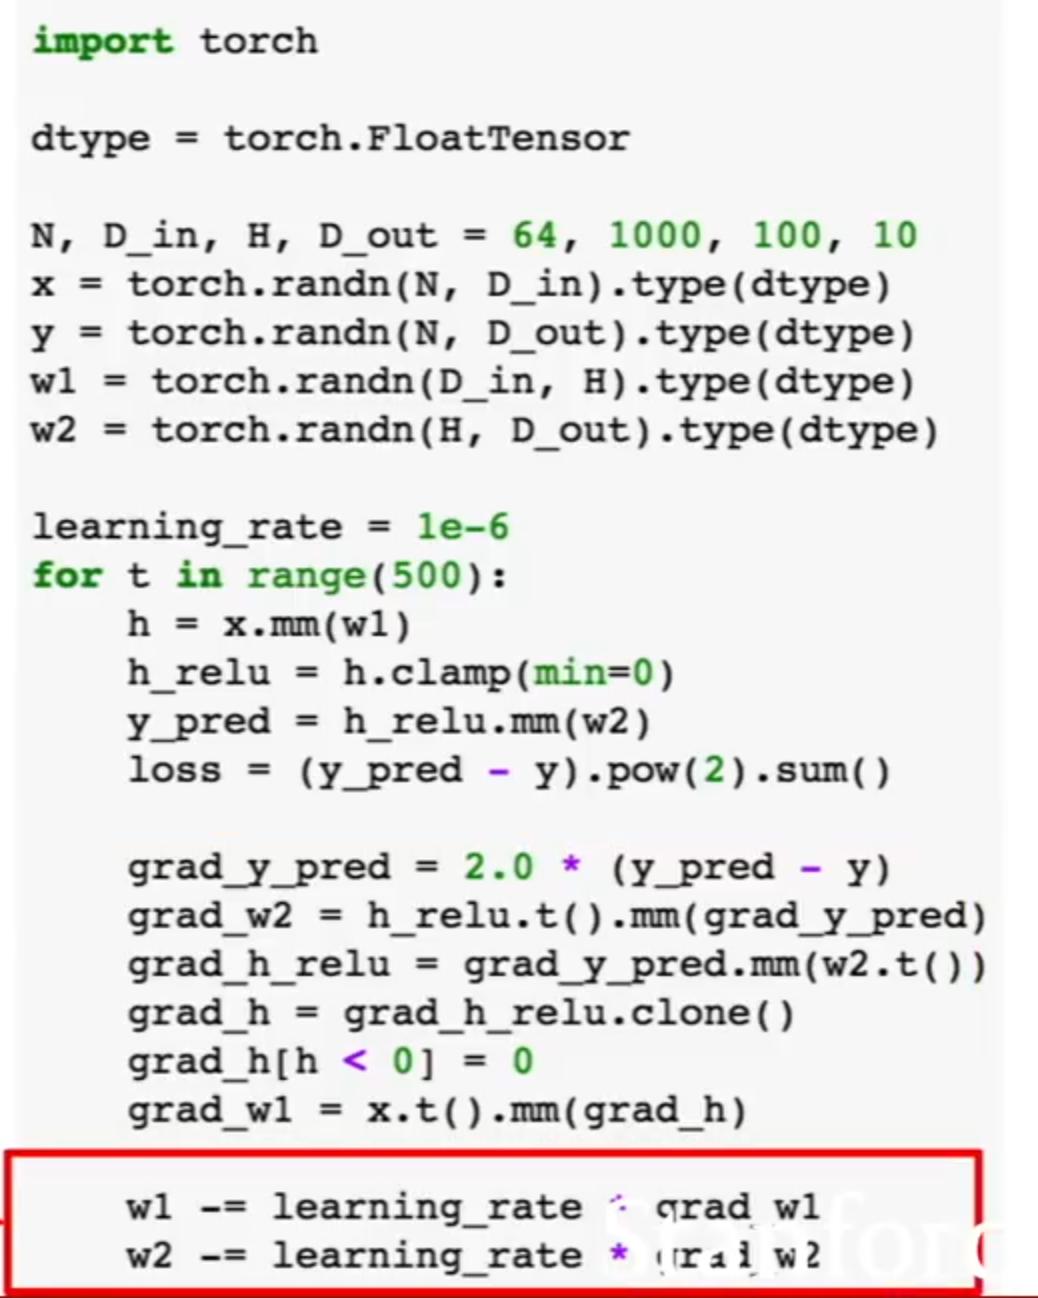
\includegraphics[width=0.5\columnwidth]{fei_fei_li/lecture_08/pytorch_tensors.png}

\paragraph{Variables + autograd}

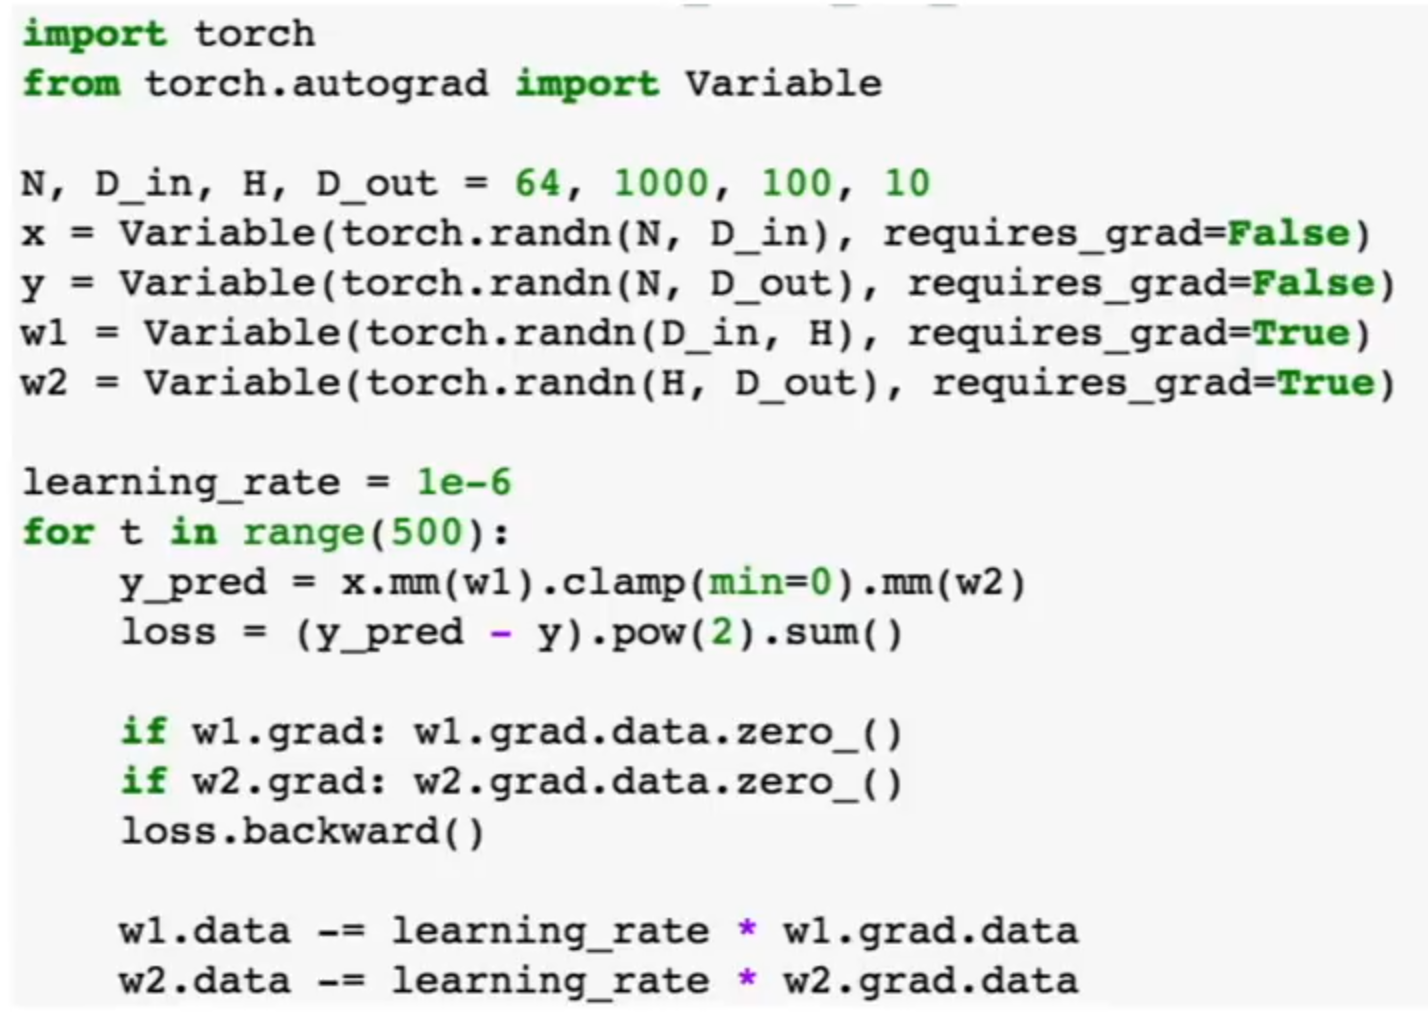
\includegraphics[width=0.5\columnwidth]{fei_fei_li/lecture_08/pytoch_variable.png}

- PyTorch we build a new graph at every forward pass which makes the code a bit cleaner
- Define autograd functions by writing forward and backwards func. imp. for Tensors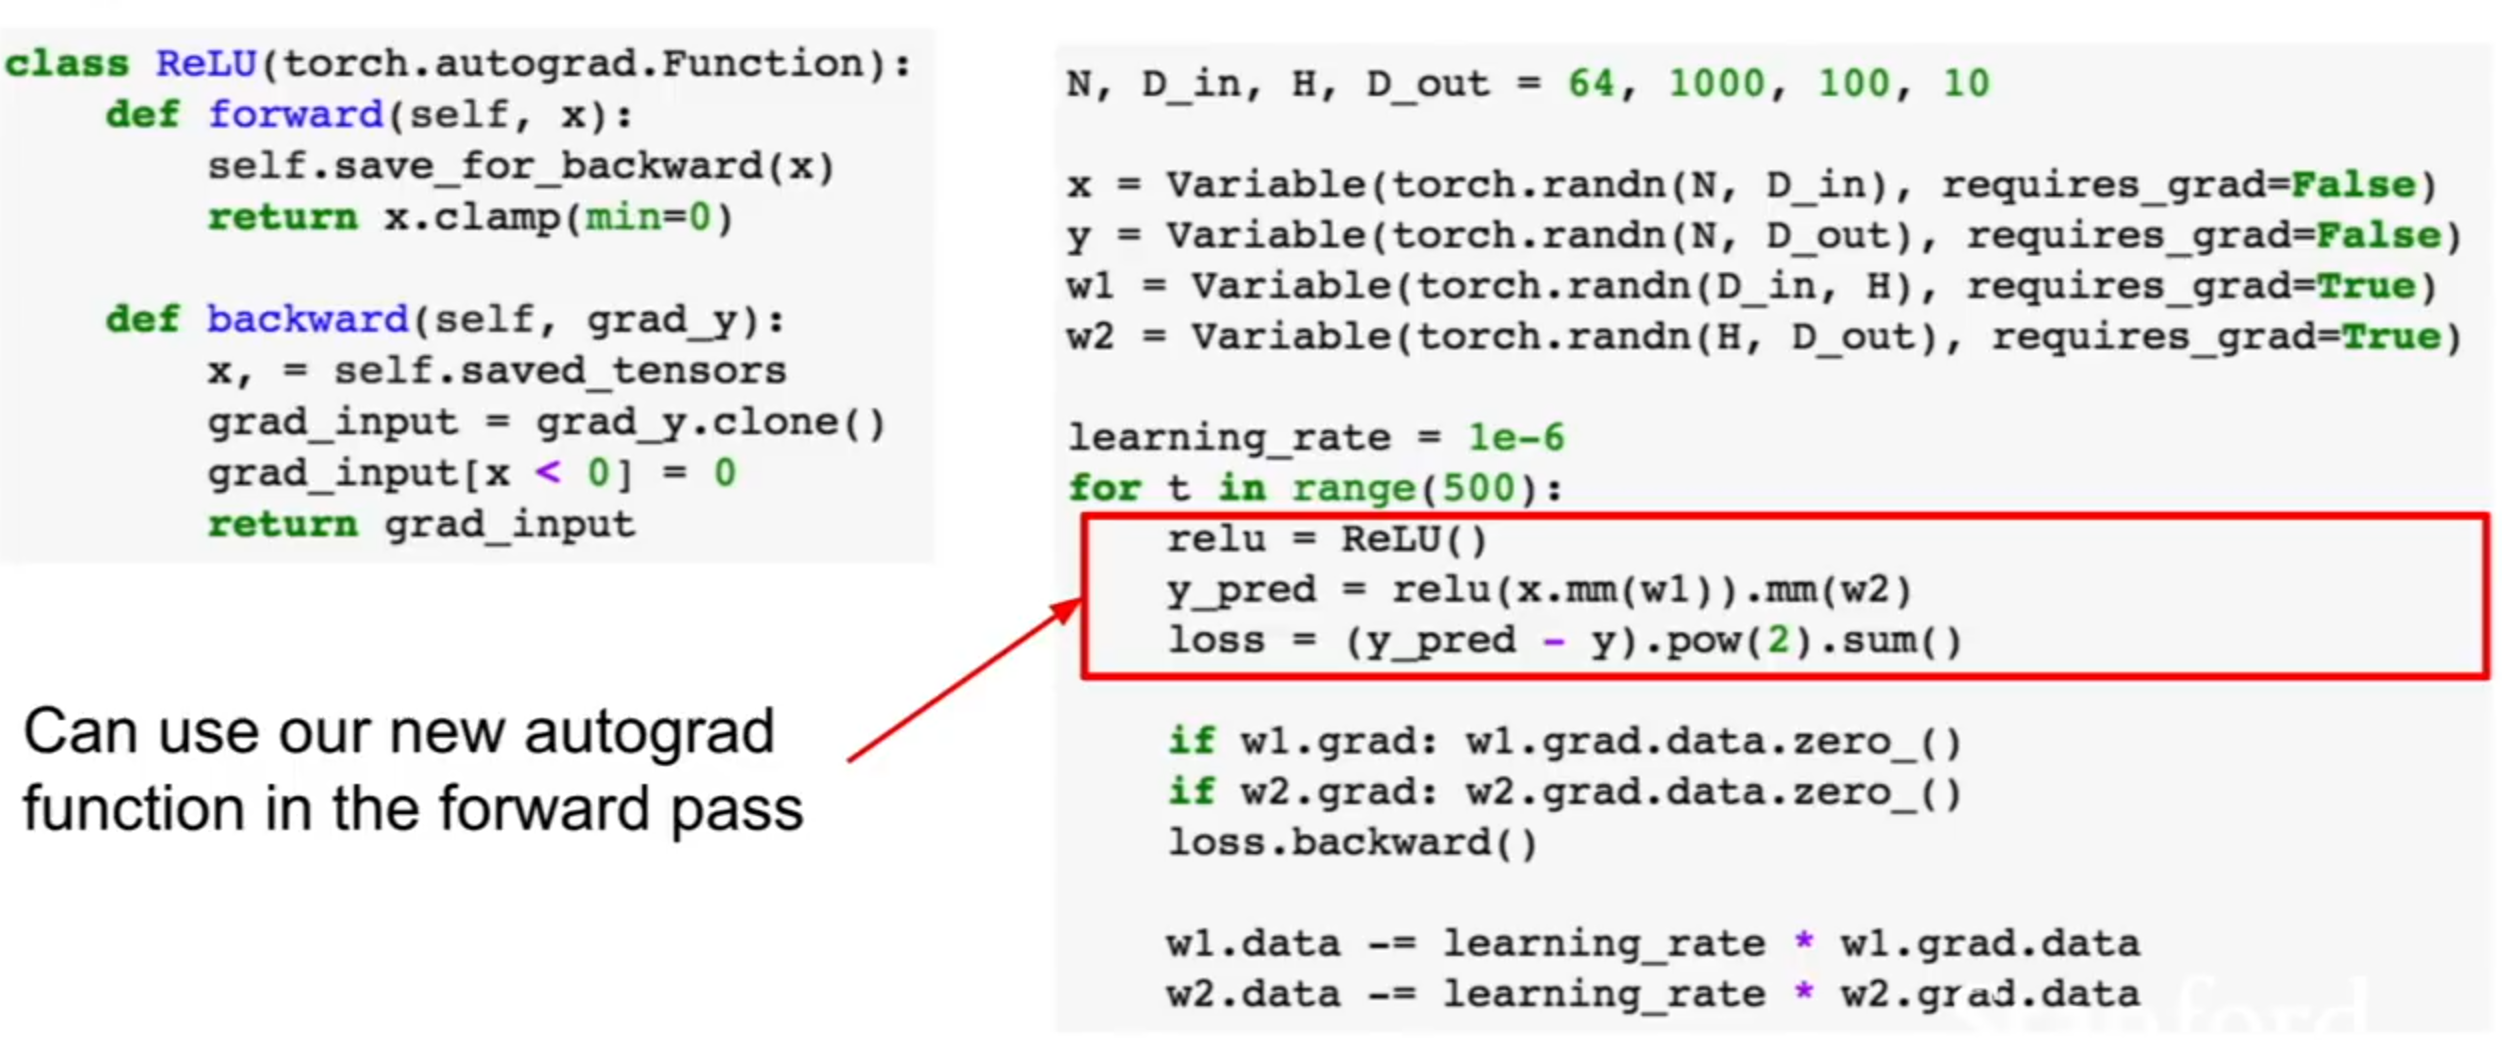
\includegraphics[width=0.5\columnwidth]{fei_fei_li/lecture_08/pytorch_autograd.png}
- we also work at the higher level:
- 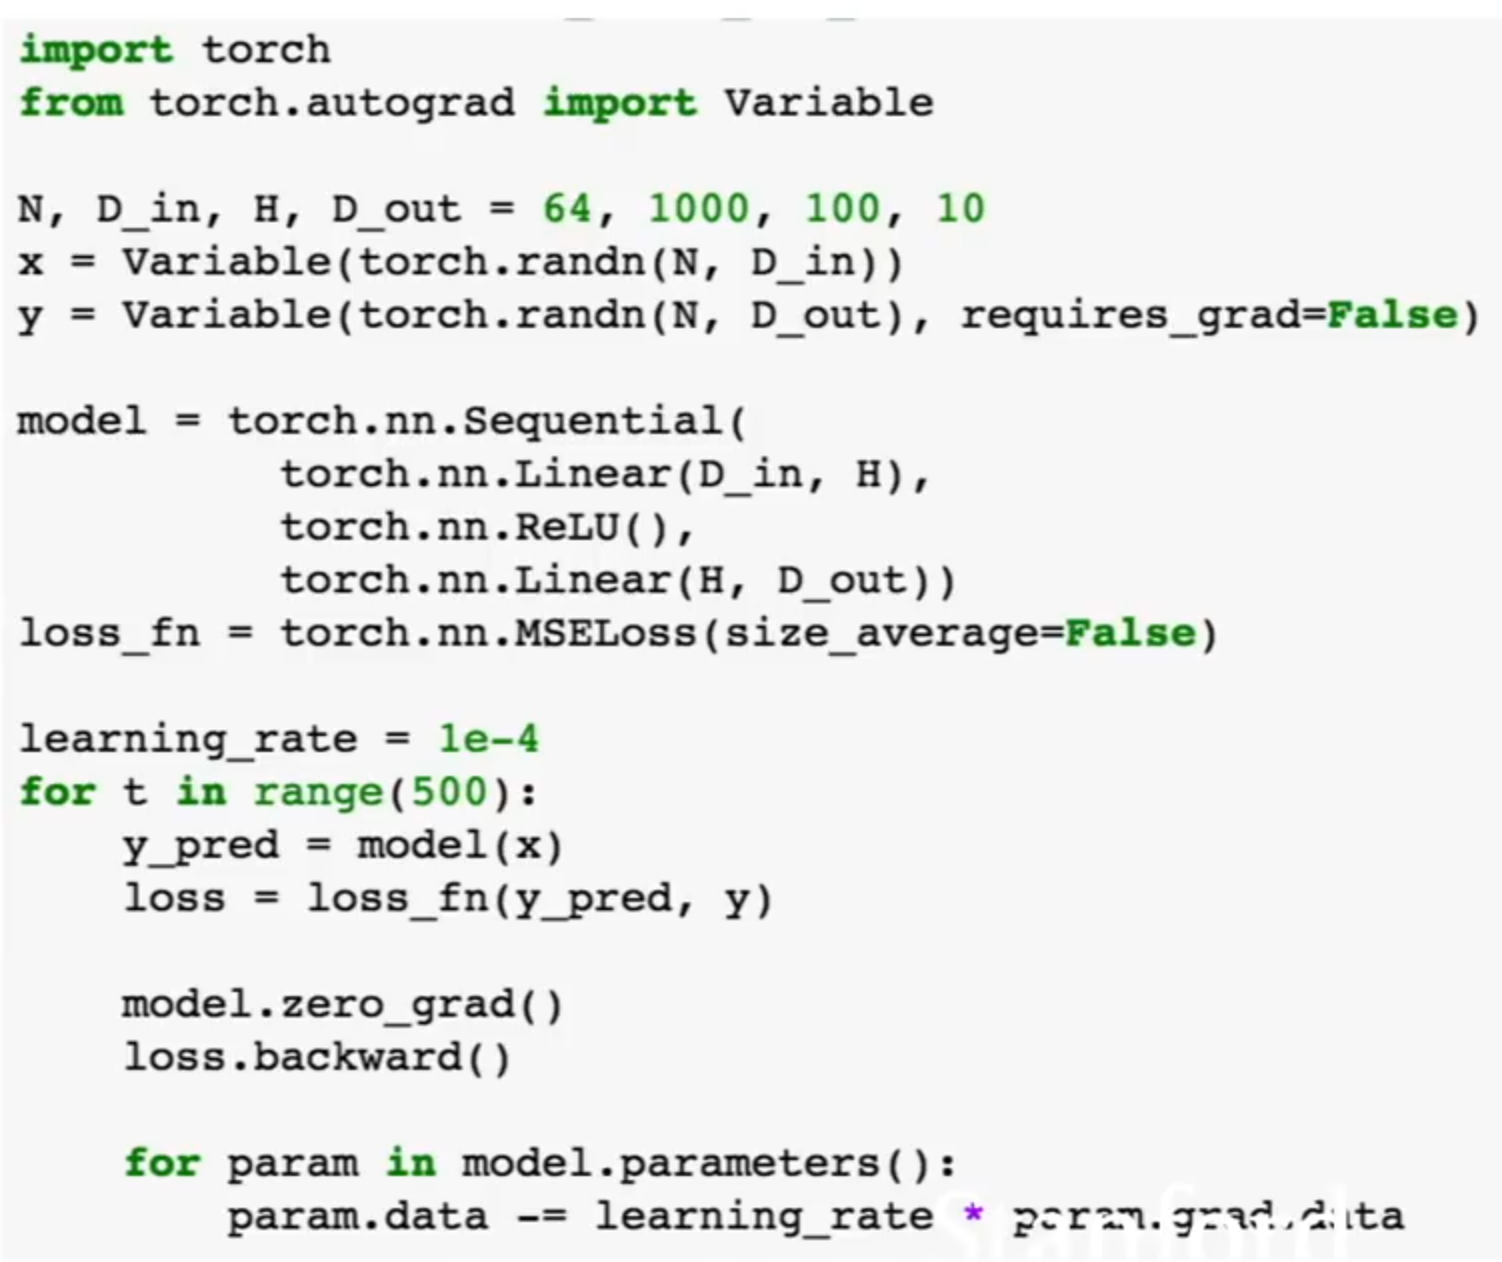
\includegraphics[width=0.5\columnwidth]{fei_fei_li/lecture_08/pytorch_nn.png}



Modules



\paragraph{DataLoader }

write a data class that knows how to load and prepare the data



\paragraph{Complete PyTorch Pipeline}

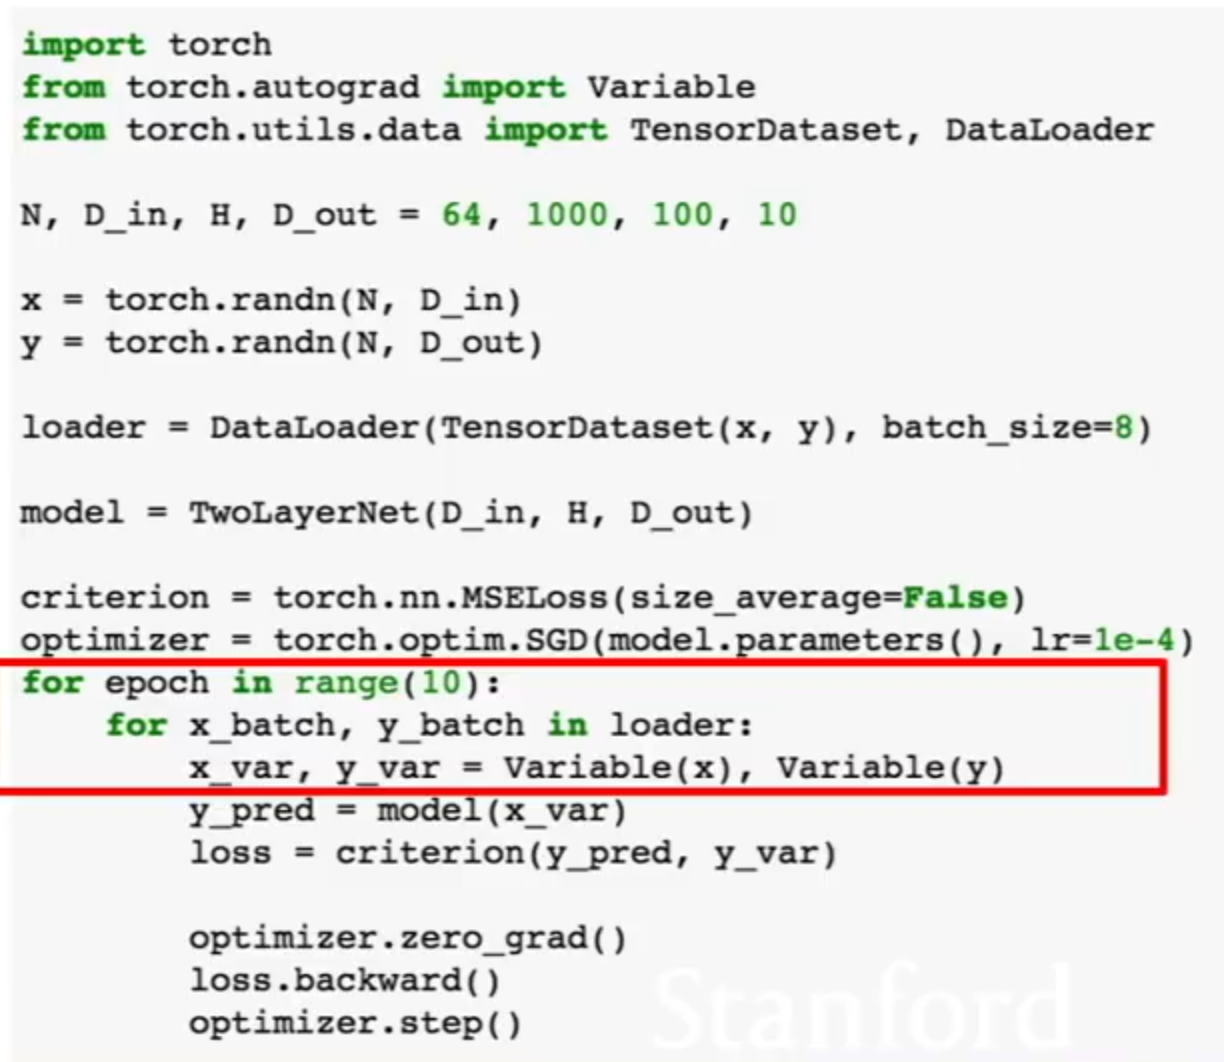
\includegraphics[width=0.5\columnwidth]{fei_fei_li/lecture_08/complete_pytorch_pipeline.png}

\subsubsection{Static vs. Dynamic Graphs}

TensorFlow - build once, run many times (static)

PyTorch - re-built at every run (dynamic)

For simple network, makes no difference

Static case

- network can do simple optimizations on the graph operations
  - more efficient - fused operations
  - more expensive upfront, but amortized over time
- you can serialize the graph and the structure of the network
  - nice for deployment scenario

Dynamic case:
\begin{itemize}
\item conditional operations
\item in tensor flow it's tf.cond() which needs to be baked into the graph
\item loops
\item RNNs is a good motivation for dynamic graphs
\end{itemize}

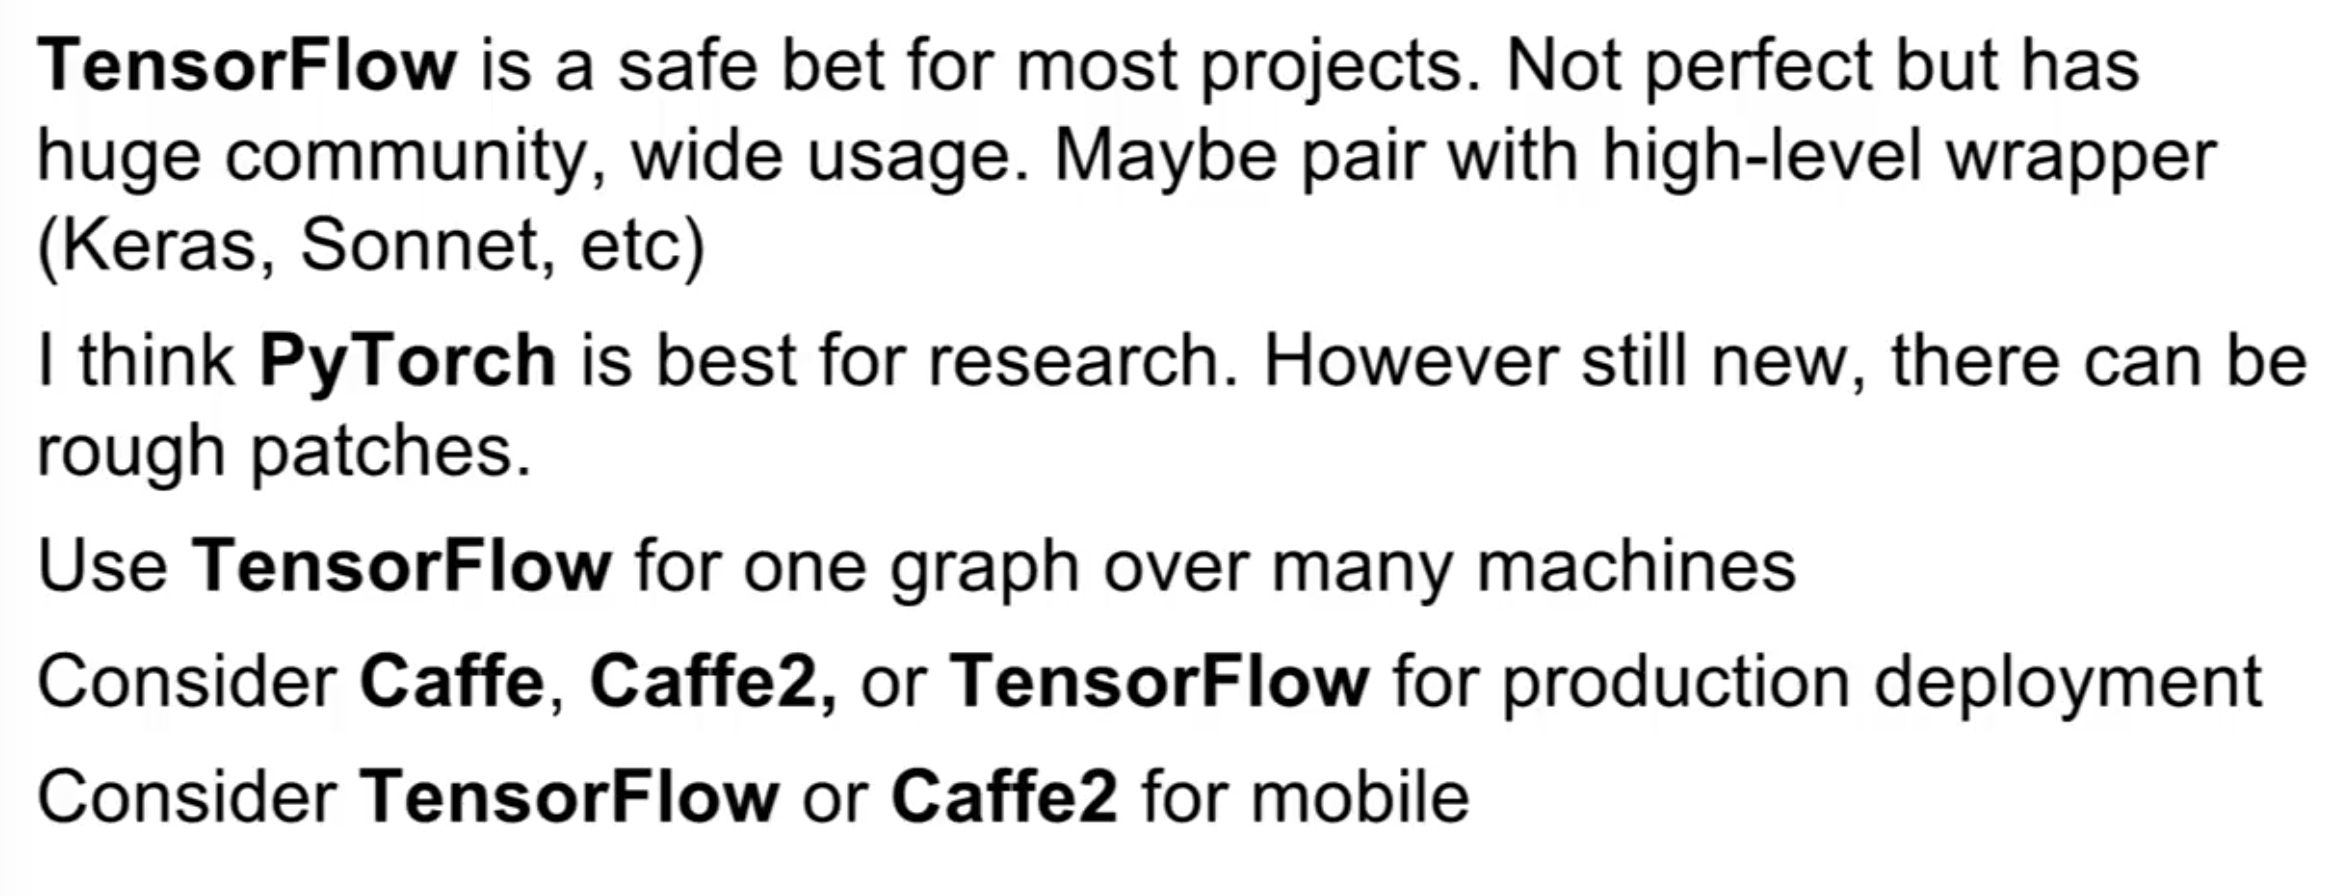
\includegraphics[width=0.5\columnwidth]{fei_fei_li/lecture_08/what_to_use.png}

\subsection{CNN Architectures}
\subsubsection{AlexNet}

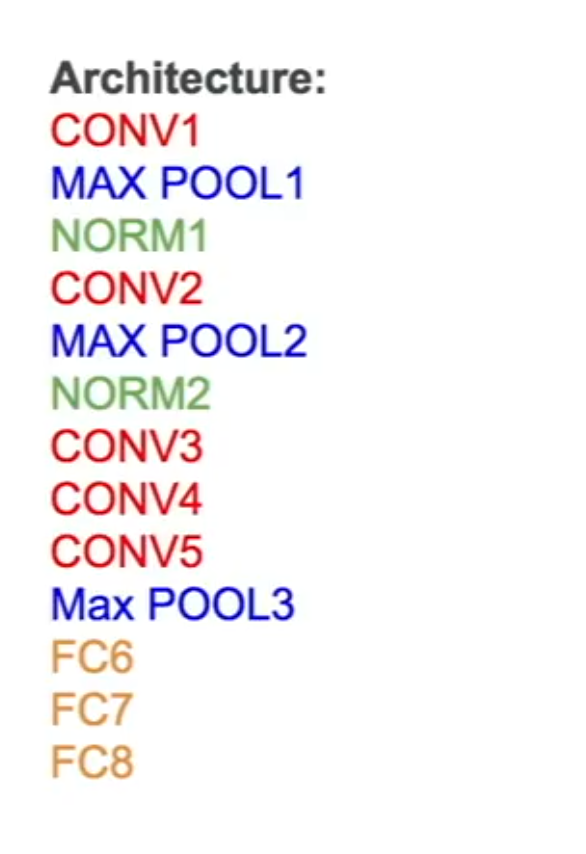
\includegraphics[width=0.25\columnwidth]{fei_fei_li/lecture_09/alex_net_2.png}

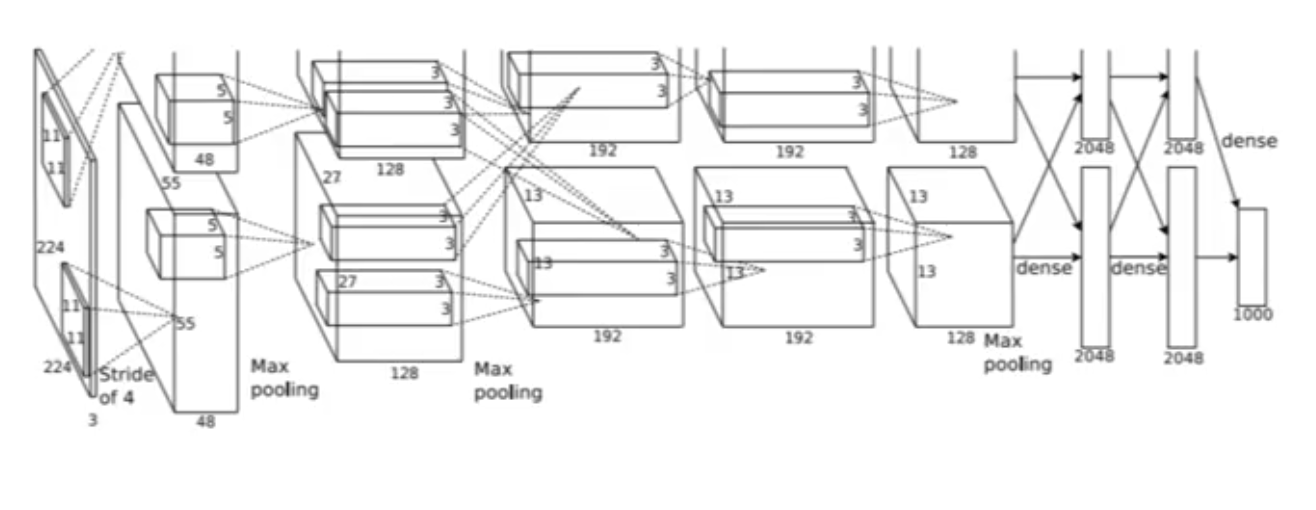
\includegraphics[width=0.5\columnwidth]{fei_fei_li/lecture_09/alex_net.png}

\subsubsection{Introduction of Deeper Networks}
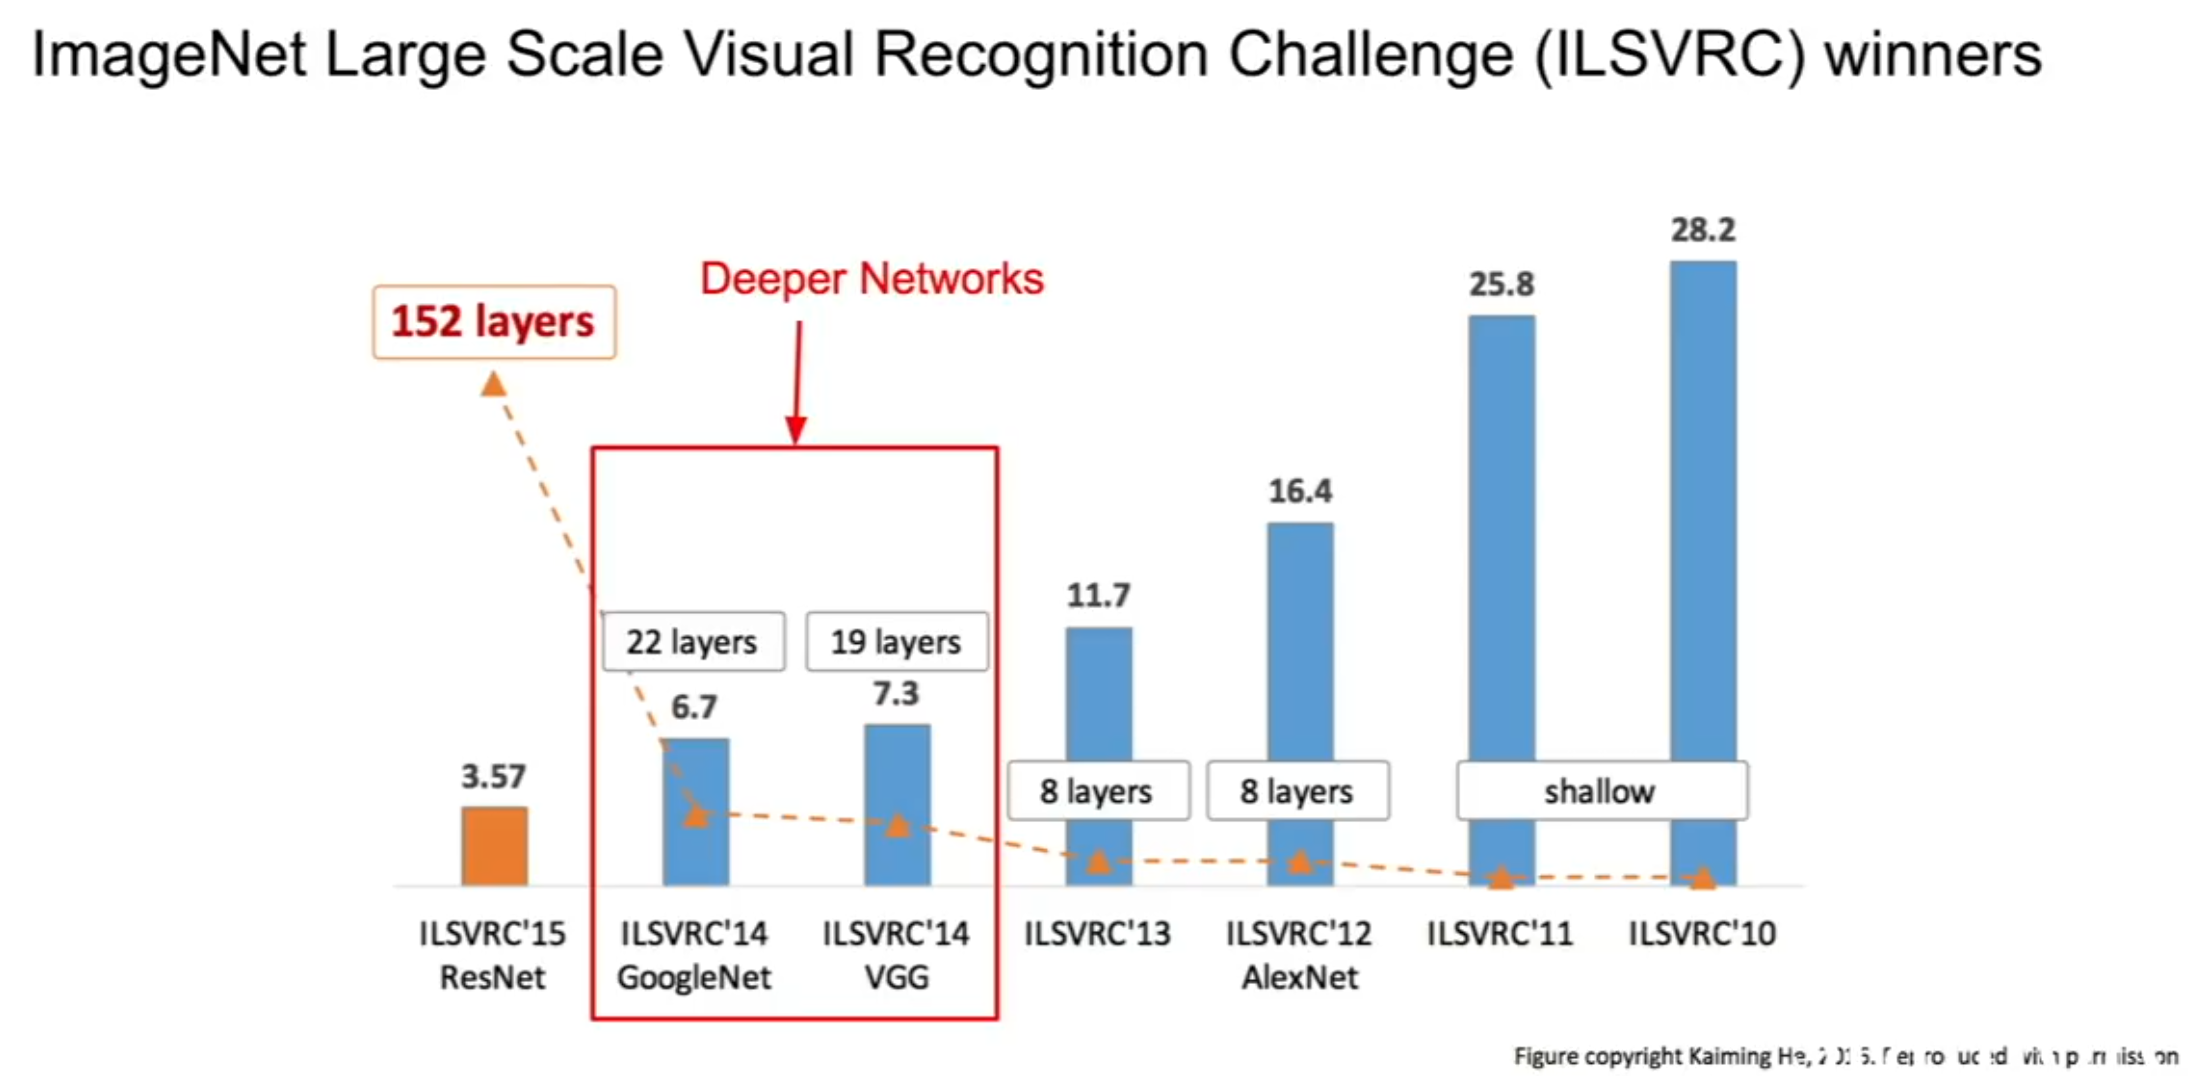
\includegraphics[width=0.5\columnwidth]{fei_fei_li/lecture_09/deeper_networks.png}

\subsubsection{GoogleNet}

- only 5 million params, x12 less than alexnet

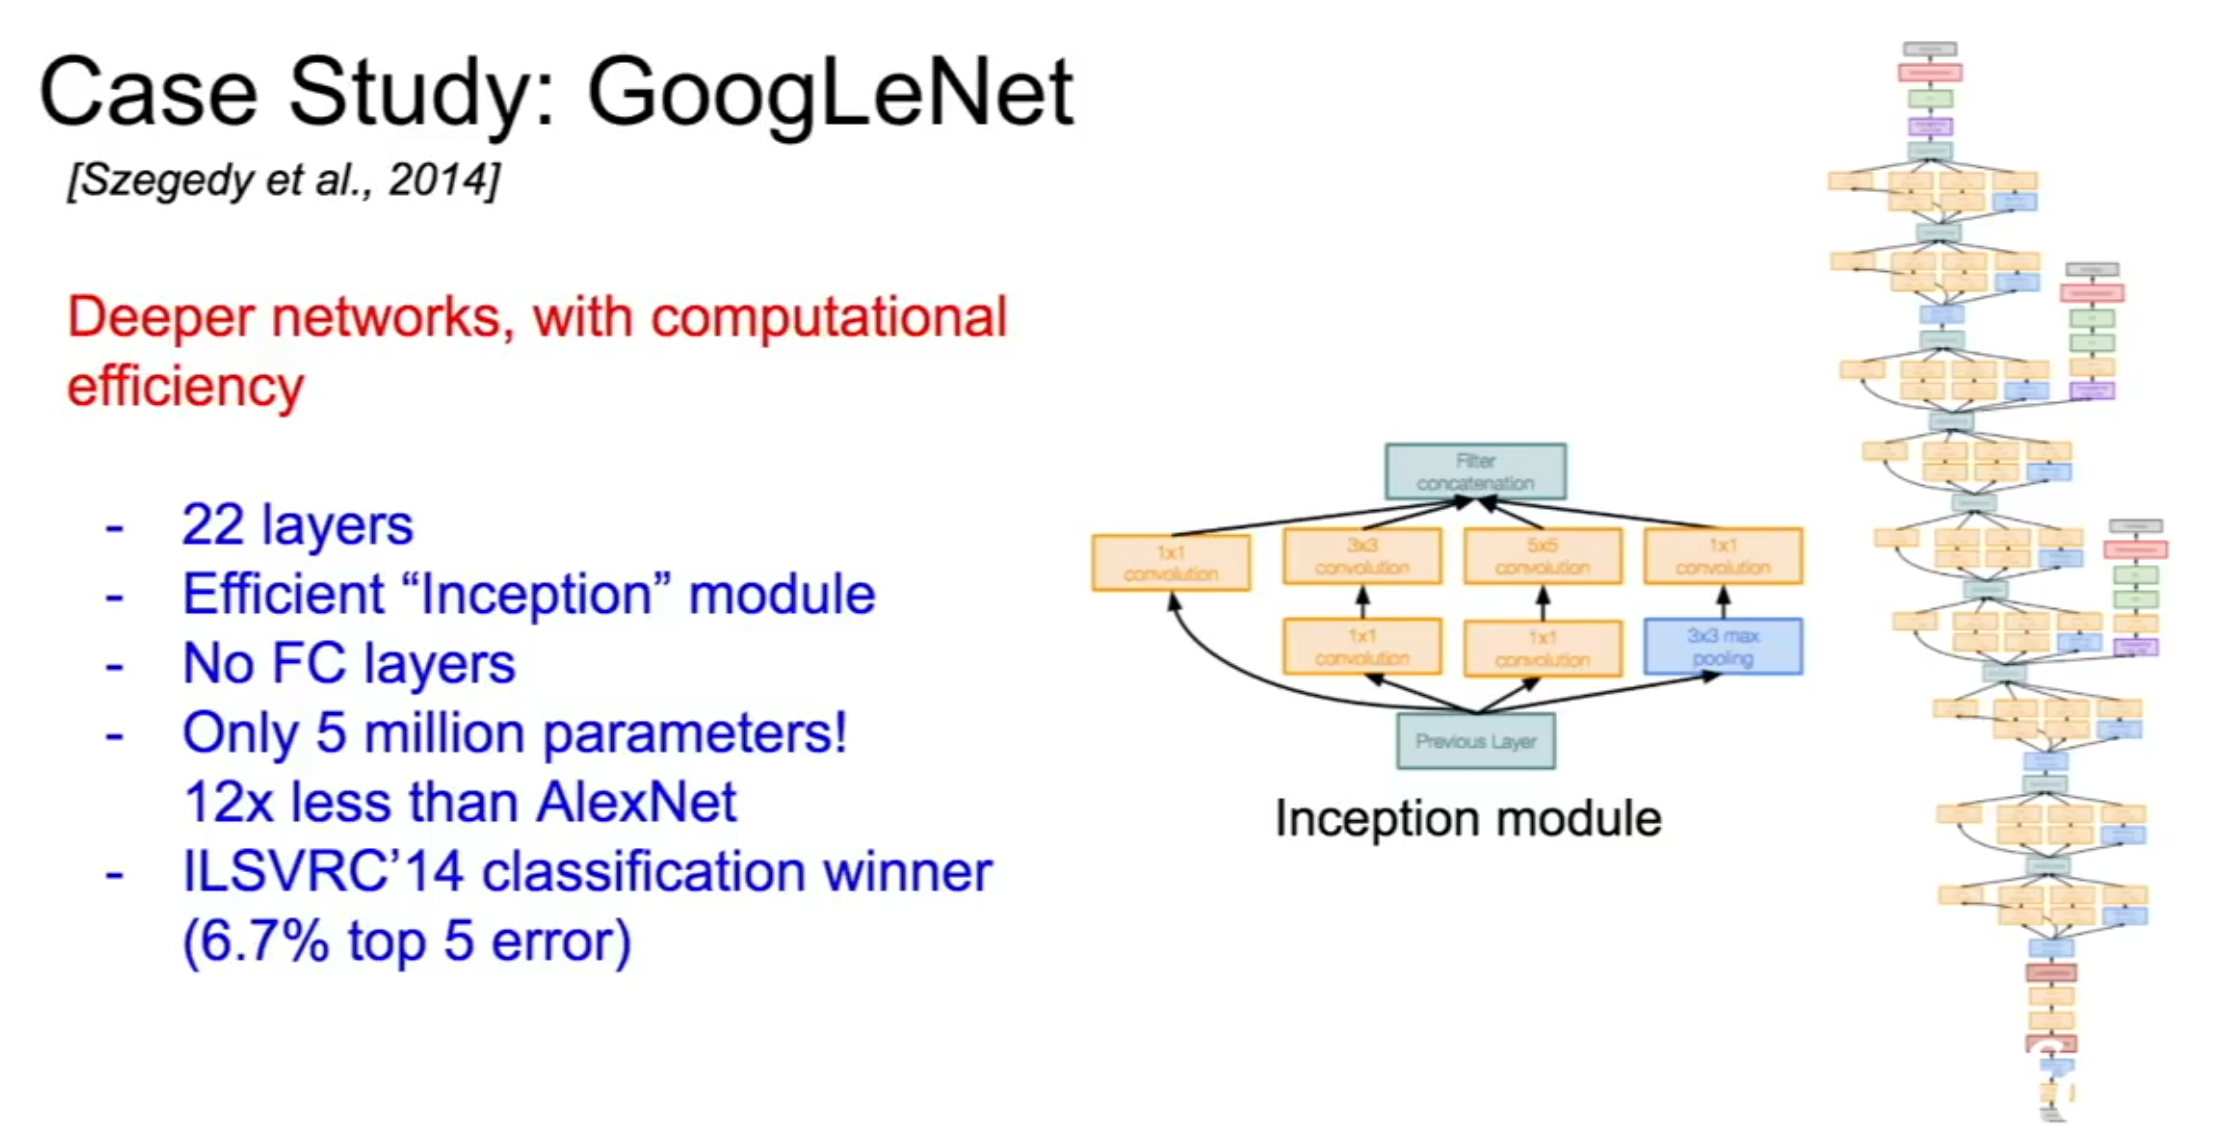
\includegraphics[width=0.5\columnwidth]{fei_fei_li/lecture_09/google_net.png}

\textbf{Inception Module}

Design a good local network topology (network within a network) and stack them together:

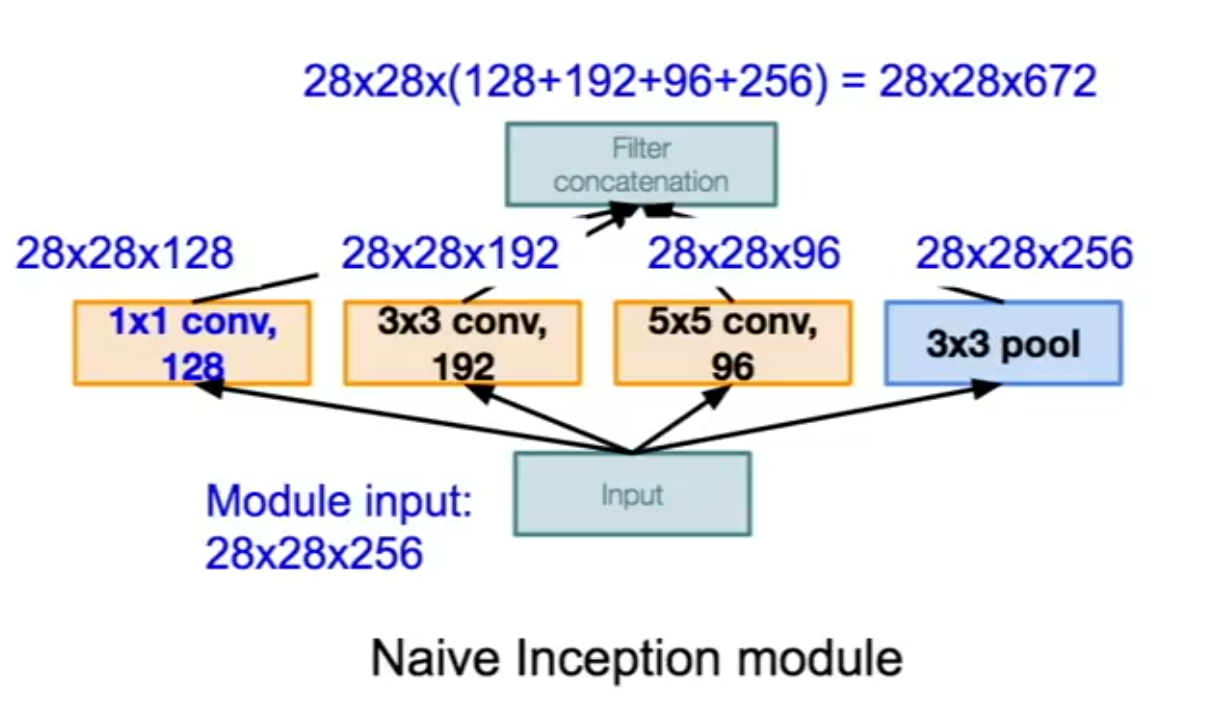
\includegraphics[width=0.5\columnwidth]{fei_fei_li/lecture_09/naive.png}

The idea is to have different operations on the same output, and then concatenate the output of these layers together.

What are the problems with this? 
\begin{itemize}
\item computational complexity - 854 mops
\item output depth - 28x28x672
\end{itemize}

How to keep this manageable?
\begin{itemize}
\item 1x1 conv with 32 filters operating on 56x56x64 $->$ 56x56x32 
\item conv layers preserve spatial information but can reduce depth
\item projecting the input to lower dimension before expensive operations:
\end{itemize}

The optimized version has 358Mops vs. 854

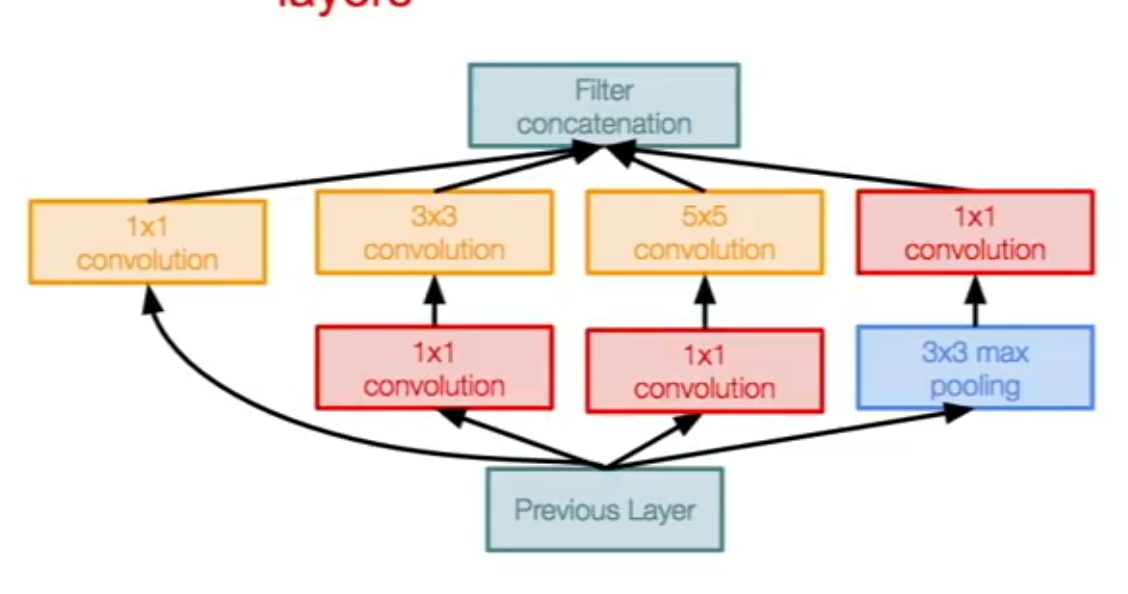
\includegraphics[width=0.5\columnwidth]{fei_fei_li/lecture_09/less_naive.png}

\paragraph{ResNet}

Revolution of depth - 152 resnet architecture

Extremely deep network using residual connections

Why is this special? 

Adding depth to a normal network $\rightarrow$ worse training response

The training error is doing worse - not because of overfitting.

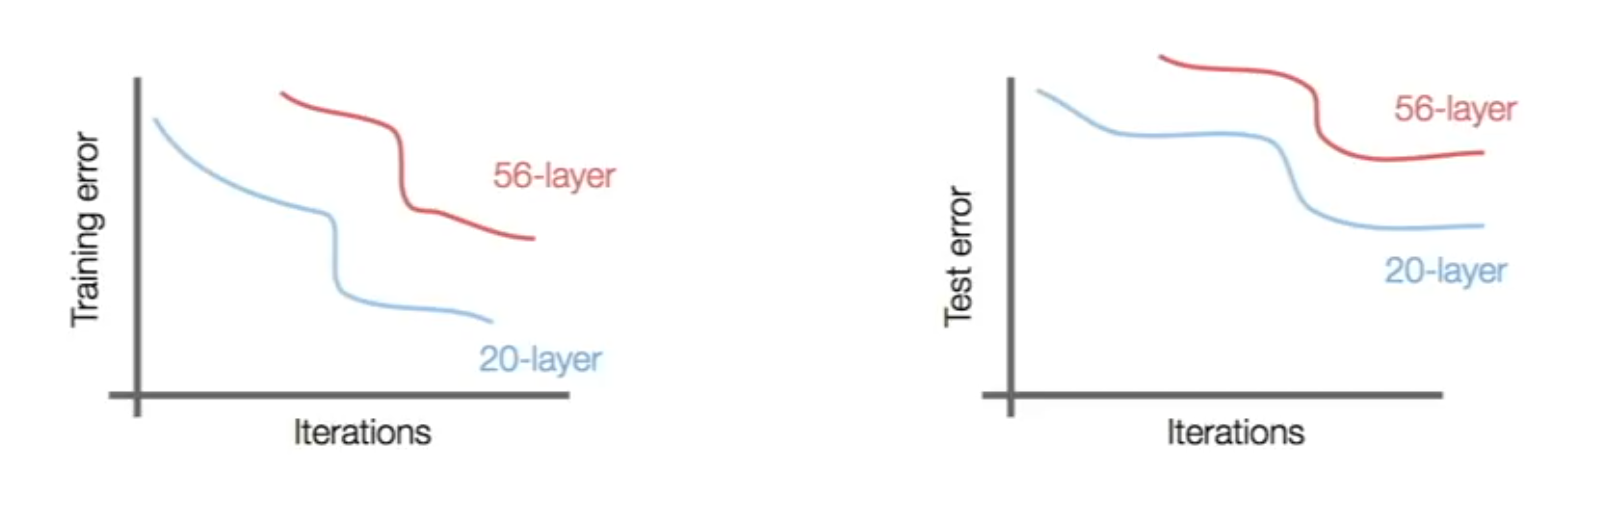
\includegraphics[width=0.5\columnwidth]{fei_fei_li/lecture_09/deep_error.png}

The problem is an optimization problem - harder to optimize

Reasoning - a deeper model should perform just as well a shallower model - for example, train 20 layer model, copy the params, add 20 more layers of identity

$\Rightarrow$ I really do not understand this "residual"

- Were able to train very deep networks without degrading
- Deeper networks can now achieve lower training error - better gradient propagation

\subsubsection{Complexity}

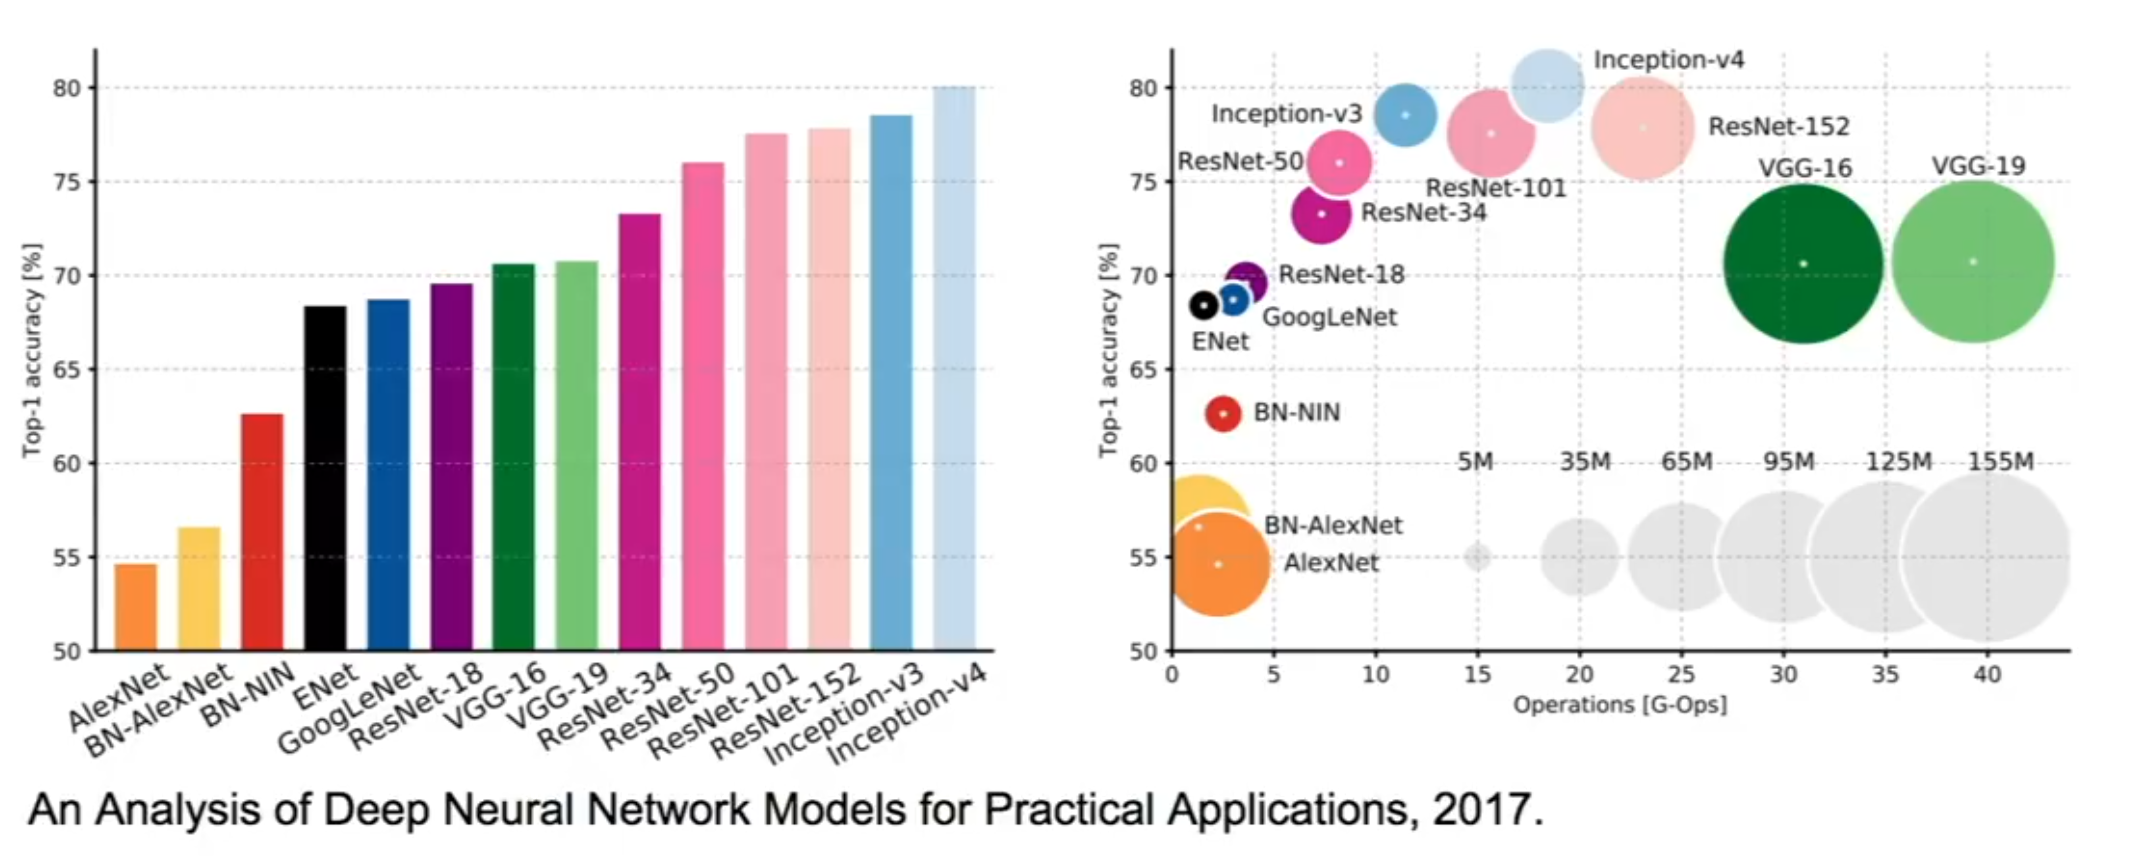
\includegraphics[width=0.5\columnwidth]{fei_fei_li/lecture_09/complexity.png}



Developments on top ResNet: 

- Huang 2016 - Deep Networks with Stochastic Depth
  - reduce vanishing gradients and training time through short network training
  - drop layers randomly at every pass, use identity
  - use full network at test time

Fractal Net

- motivation: transitioning to residual representations are not necessary

Densely Connected Convolutional Networks

Recap of CNN architecture: 

\subsubsection{More Insights of The ResNet Arch}

we pass the input through conv blocks (conv + relu)  and then add the input to the output of these blocks

if the weights are 0 - it's simply identity

interpretation of l2 regularization of the network - encourages the model to drive unneeded layers

Gradient flow in backward pass:

- addition gradient will stream and fork along two different paths
- upstream gradient will have direct connection - gradient super highway

Also DenseNet and FractalNet allow for easy gradient pass through the network



\subsubsection{More Insight on Architectures }

AlexNet and VGG have a lot of params in fully connected layers

\textbf{AlexNet}

- ~62M params -> out of which most live in a few layers:
  -  FC6 256x6x6 -> 4096: 38M Params
  - FC7 4096 -> 4096: 17M Params
  - FC7 4096 -> 1000: 4M Params
  - 59M params in 3 layers

\subsection{Recurrent Neutral Network }

% 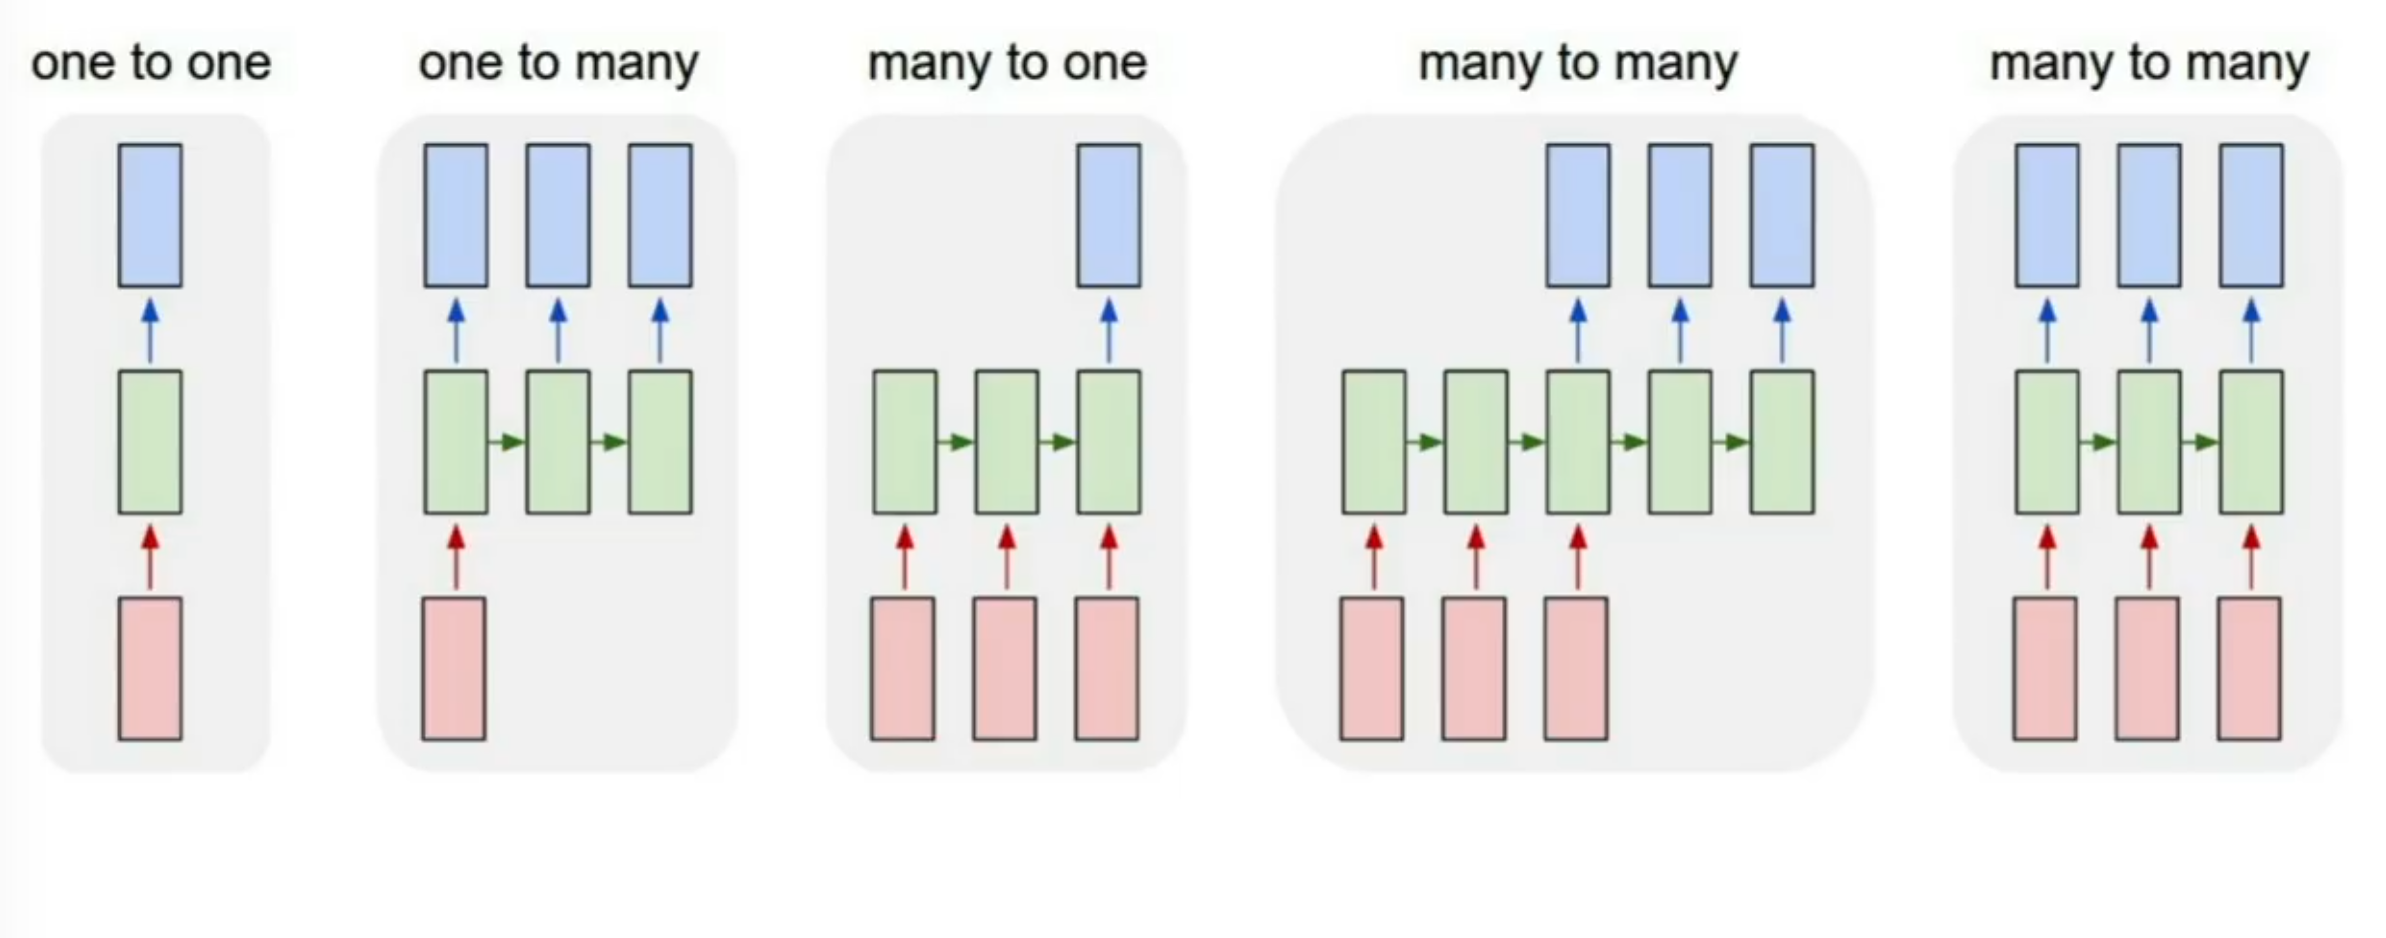
\includegraphics[width=0.15\columnwidth]{fei_fei_li/lecture_10/data_flows.png}

We can have tasks that require a different data flow through the networks. 

The vanilla one to one connection is called  feed-forward network. 

one to many $\rightarrow$ image captioning - for example, image to sequence of texts

many to one $\rightarrow$ variable size input -> for example, labelling text, or labelling video

many to many (1) $\rightarrow$ machine translation, variable length sequences of inputs and outputs

many to many (2) $\rightarrow$ video classification on frame level

\subsubsection{RNN}

% 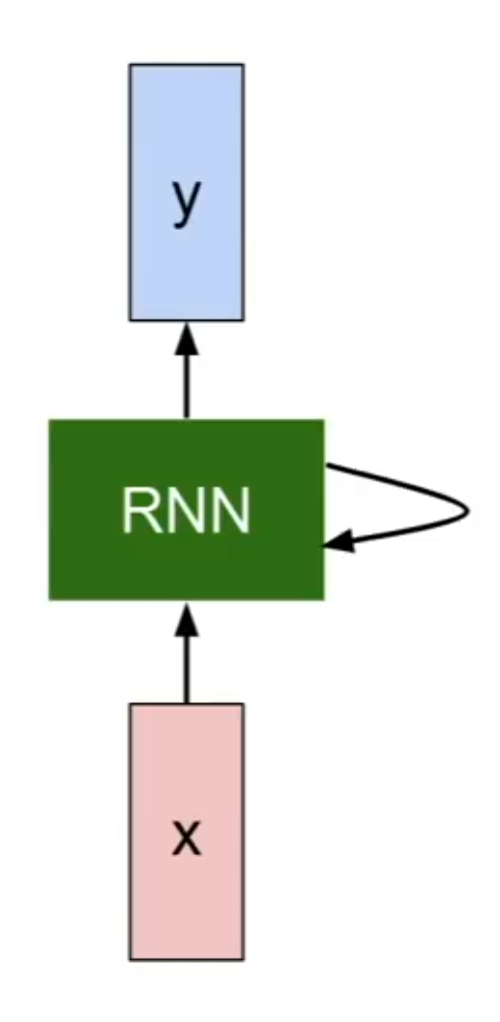
\includegraphics[width=0.5\columnwidth]{fei_fei_li/lecture_10/rnn.png}

$$h_t = f_W(h_{t-1},x_t) $$

$h_t$ new state

$h_{t-1}$ - old state

$x_t$ -  input vector at some time step

$f_W$ some function with params

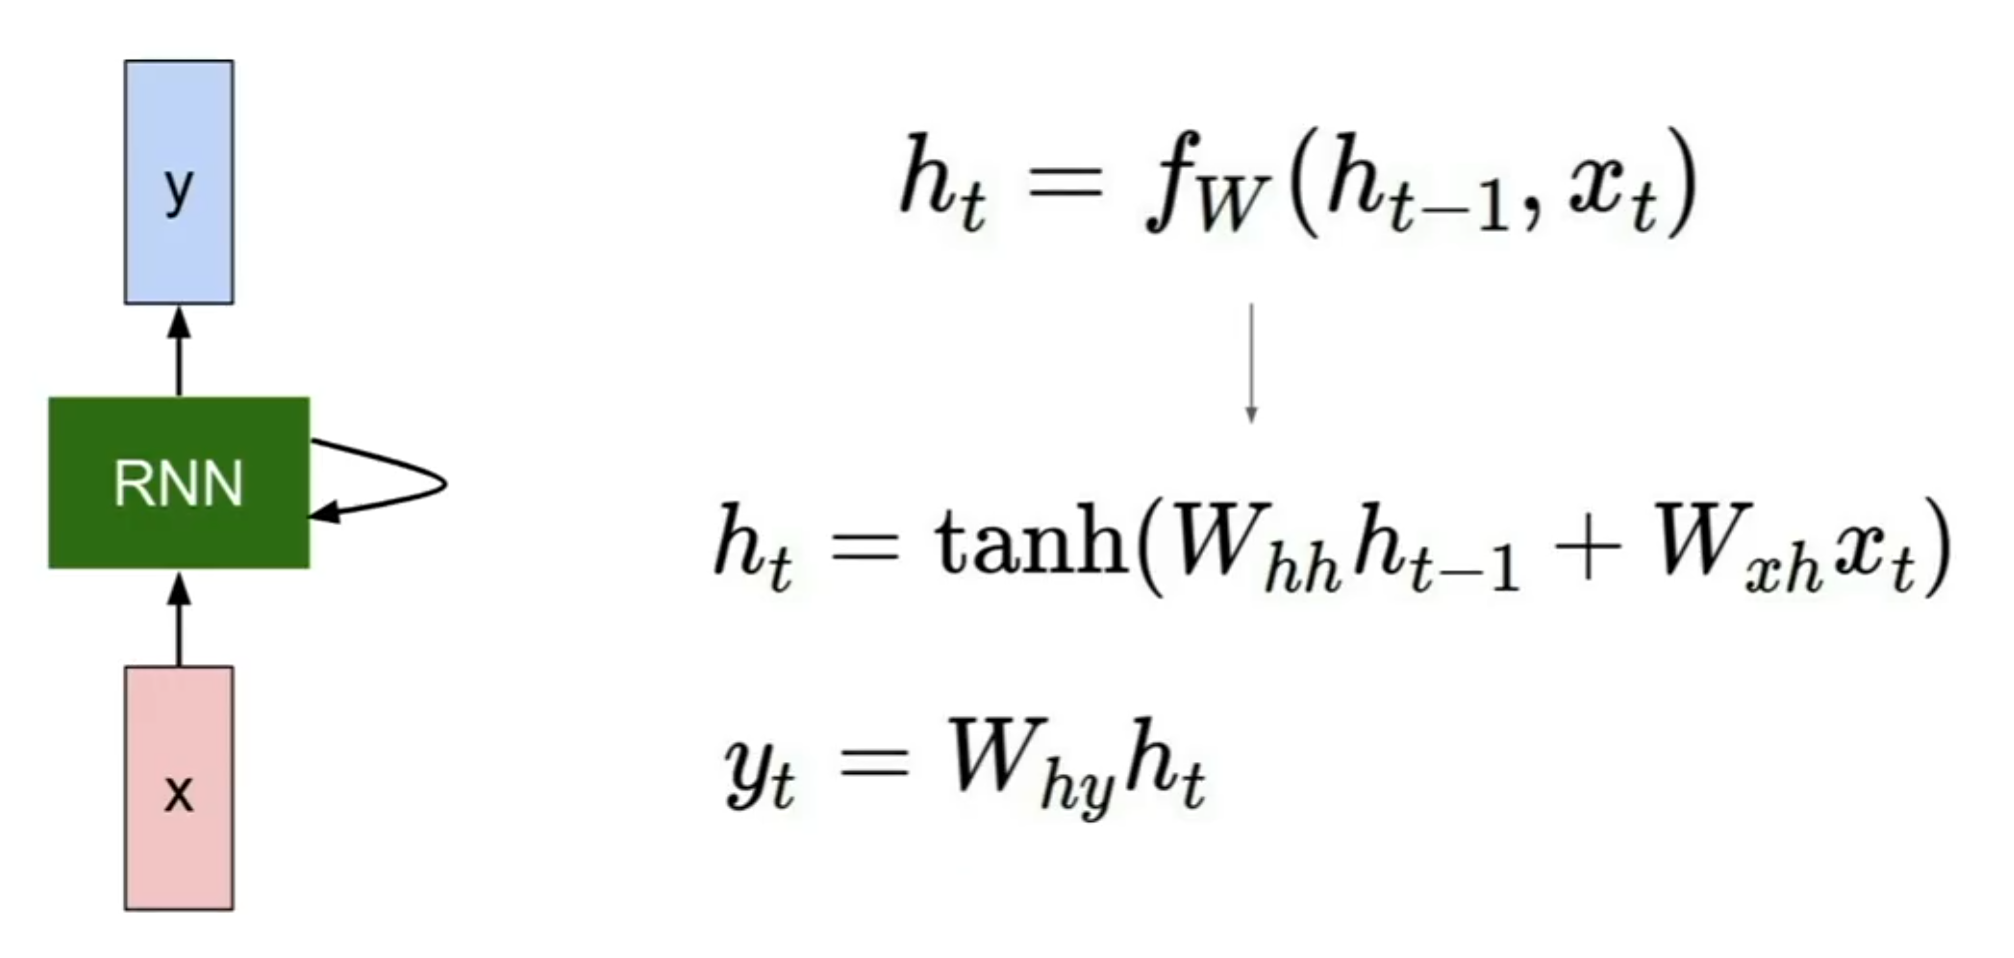
\includegraphics[width=0.5\columnwidth]{fei_fei_li/lecture_10/rnn_formulation.png}

RNN Unrolling: W remains constant throughout the optimization

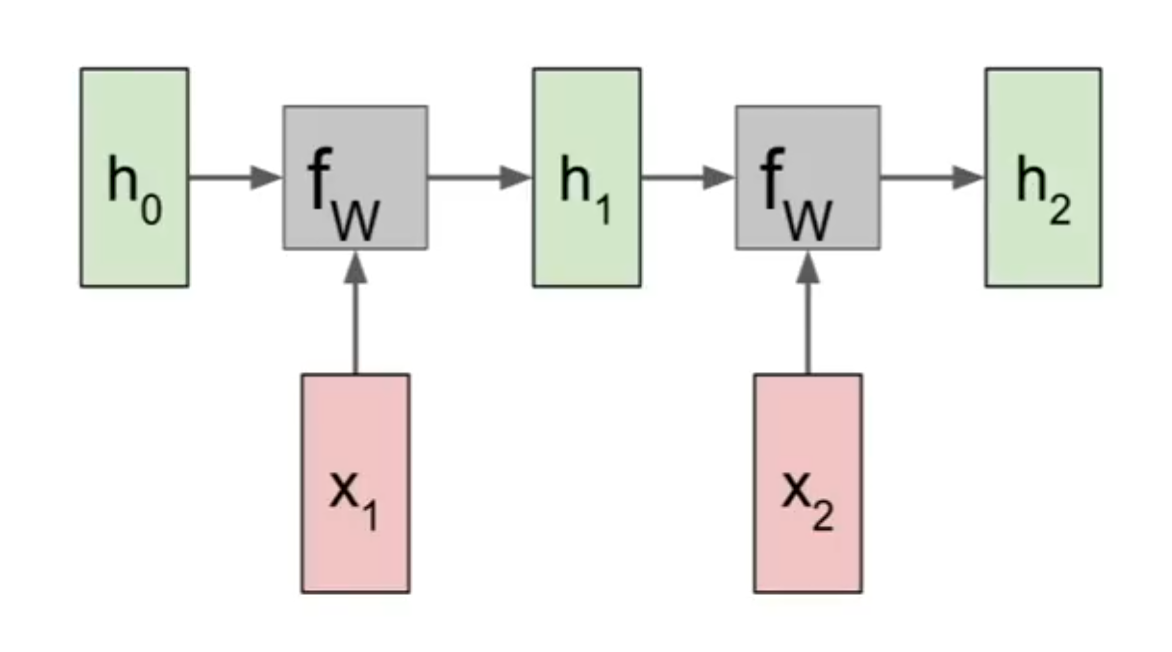
\includegraphics[width=0.5\columnwidth]{fei_fei_li/lecture_10/rnn_unrolling.png}

Many to many - we can get output at every step

Many to one - we will get output based on the final state at the end of the input

One to many - unroll the graph for each cel in the output

Sequence to sequence: encoder and decoder

Encode input sequence in a single vector

Decoder network - one to many - produce output sequence from single input vector

\subsubsection{Example: Character-level Language Model}

Vocabulary: [h,e,l,o]
Training:"hello"

Sampling from the model: seed the model with input

the output layer will have scores with a probability distribution

we can sample from it with softmax and synthesize the next sequence

why sample? 

hard max probability

but sampling let's you get diversity

\subsubsection{Back-propagation through time}

Forward though the entire sequence to compute loss, then backwards though the entire sequence to compute gradient

Very hard to train on long sequences.

Truncated Backpropagation through time - many people use 100 steps. 

Compute a loss over the subsequence of the data

check out min-char-rnn on github for a minimal example of rnn backprop

\paragraph{RNN Attention Models}

RNN can focus its attention on different parts of the image

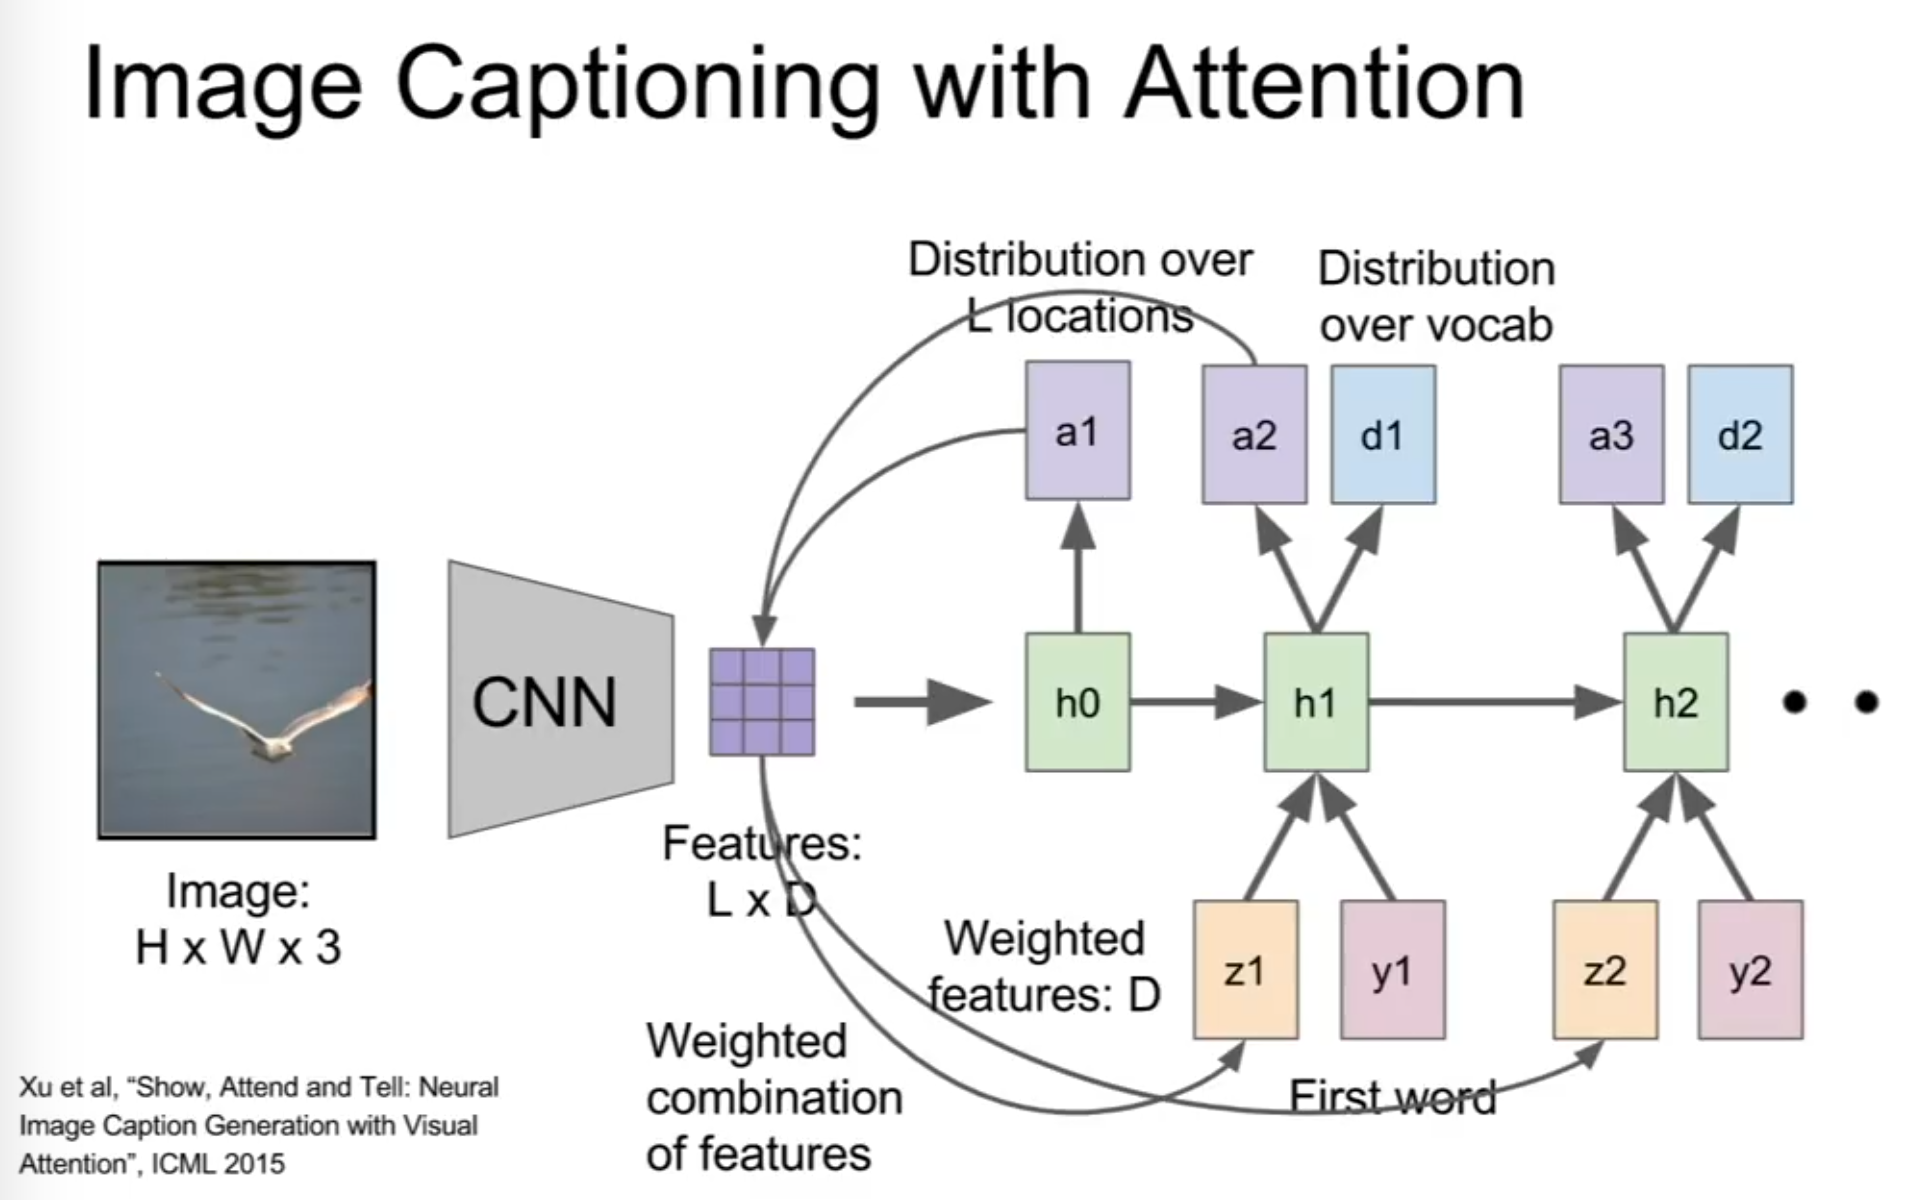
\includegraphics[width=0.5\columnwidth]{fei_fei_li/lecture_10/image_captioning_with_attention.png}

\paragraph{Multi layer RNNs}

max 4 or so

\paragraph{Back propagation of gradient through RNNs}

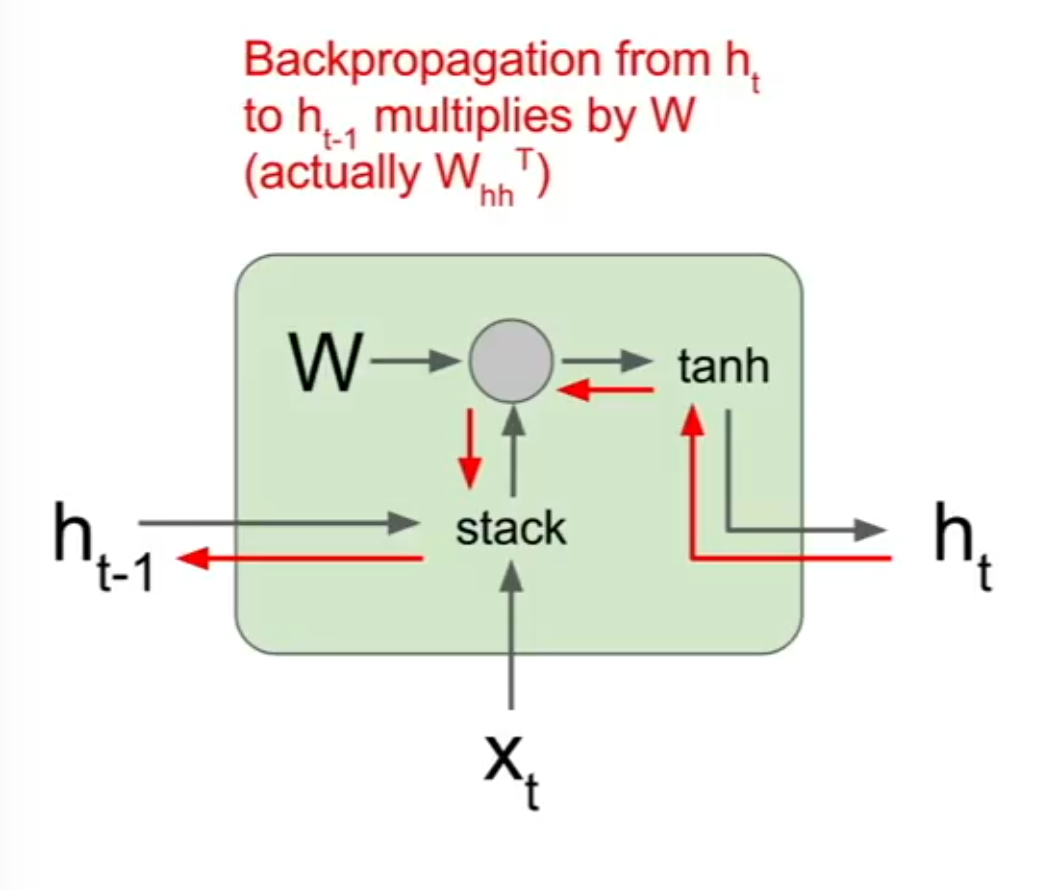
\includegraphics[width=0.5\columnwidth]{fei_fei_li/lecture_10/back_prop_rnn.png}

Gradient through multiple RNN cells: 

Computing the gradient with respect to $h_0$ - we get multiple factors of the $W$ matrix, which can be undesirable. 

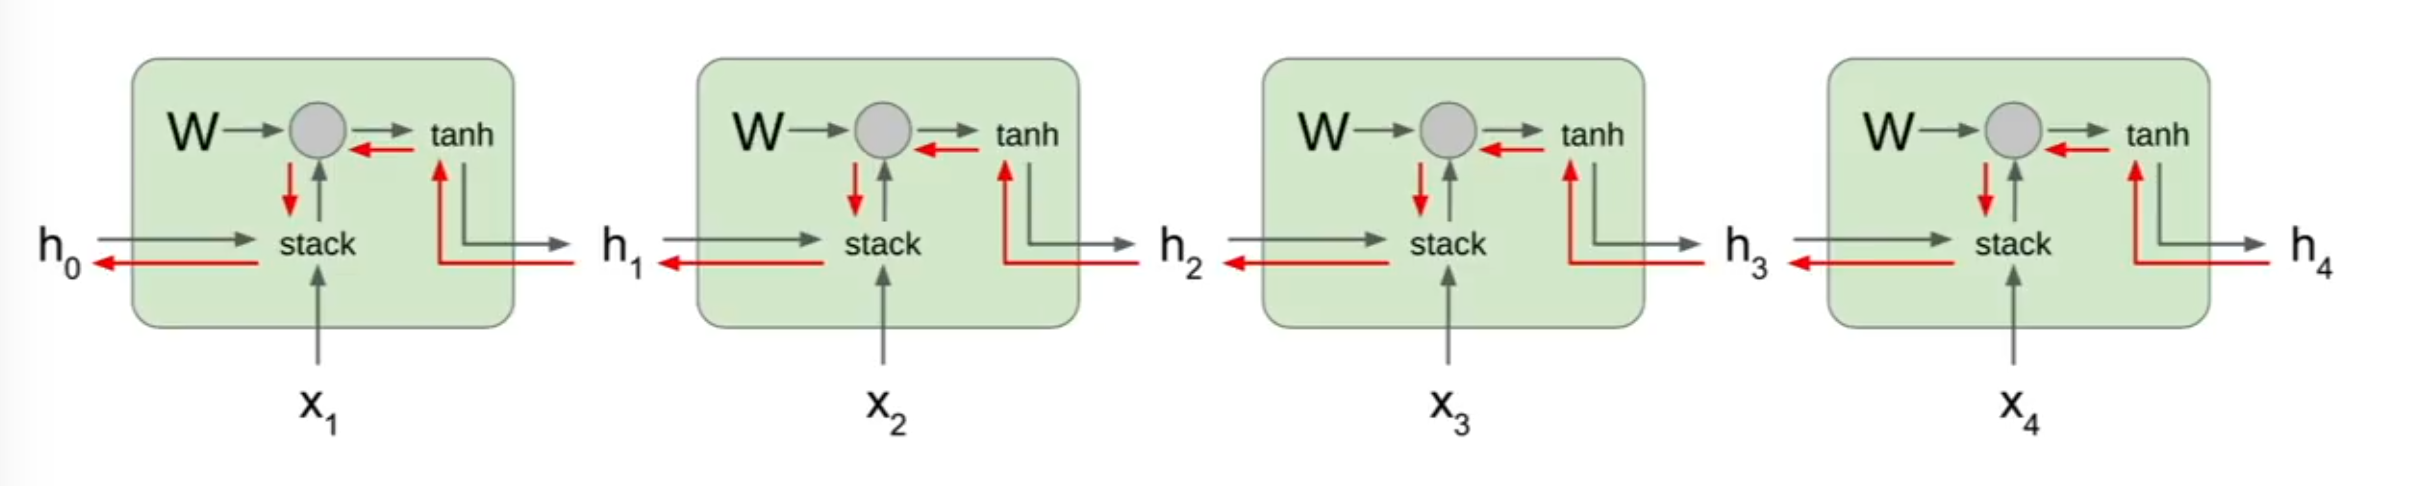
\includegraphics[width=0.5\columnwidth]{fei_fei_li/lecture_10/backprop_multi_layer.png}

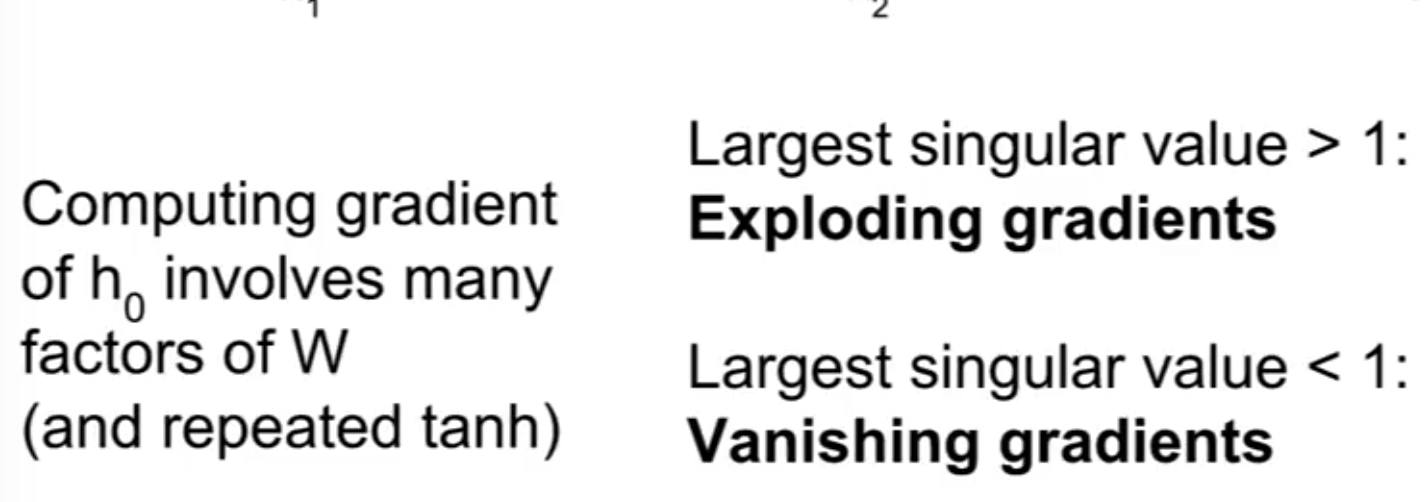
\includegraphics[width=0.5\columnwidth]{"fei_fei_li/lecture_10/gradients.png"}

trick: gradient norm > max threshold, gradient is normalized by its norm

\subsubsection{LSTM}

Long short term memory

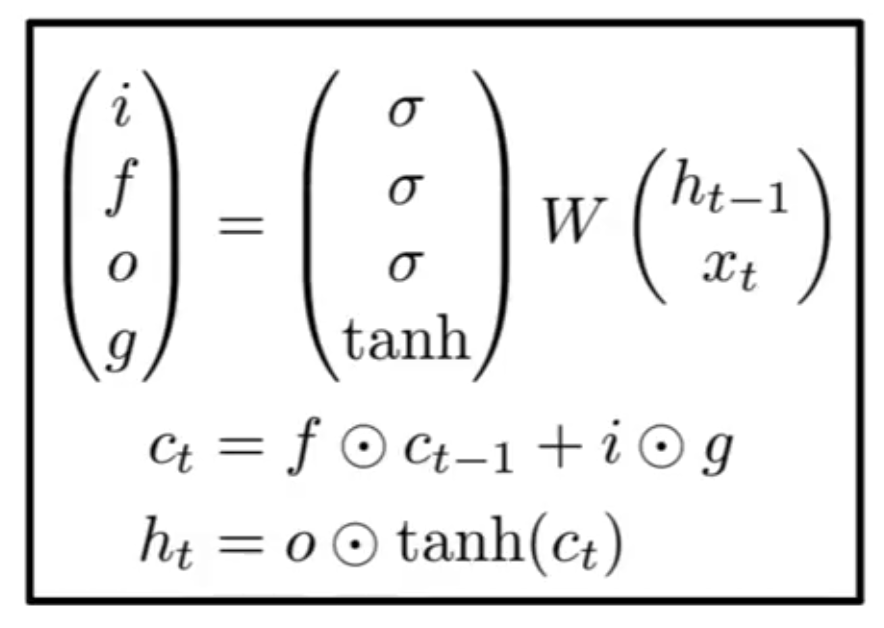
\includegraphics[width=0.5\columnwidth]{fei_fei_li/lecture_10/lstm.png}

better gradient flow properties

$c_t$ cell state - keeps track of the internal state of the cell

we use input to compute the gates i - g

we expose part of the state as the hidden state at the next time step

f - forget gate, wether to erase the cell.

a vector of 0 and 1 which decides for each element wether to use it or not

(element-wise product)
i - input gate, wether to write the cell

similar, but for g gate
g - gate gate - how much to write to cell

o - output gate - how much to reveal cell

at every time step we can remember or forget the internal state, and increment or decrement the state of the cell by 1.

now we squash this into the range of [-1,1] with tanh and the output gate is coming through a sigmoid

the forget gate is coming out of a sigmoid - the forget gate is guarnteed between [0,1]

the output do not flow through tanh

and also there's direct gradient propagation, but i'm not sure about this LSTM stuff

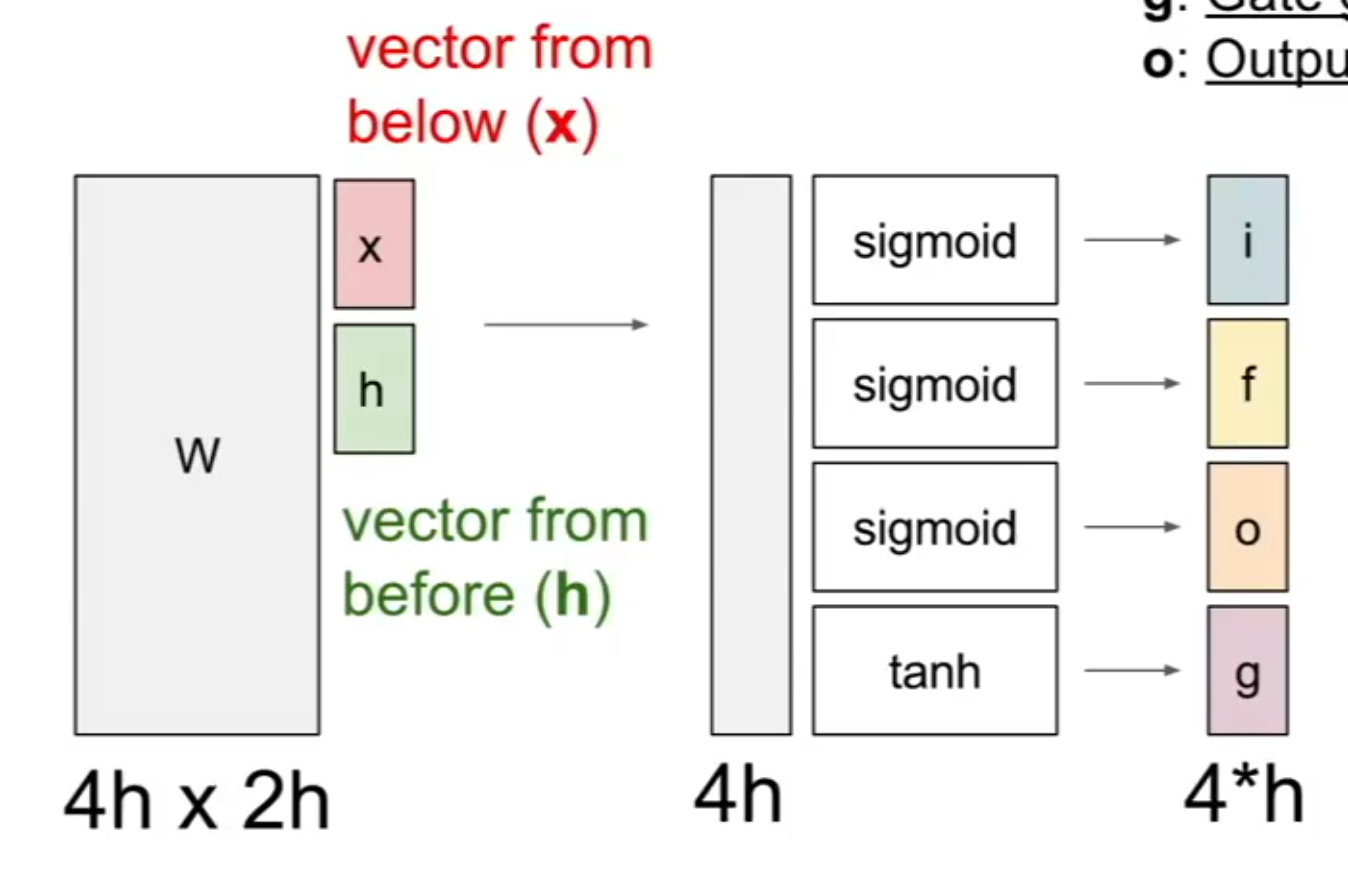
\includegraphics[width=0.5\columnwidth]{fei_fei_li/lecture_10/lstm_arch.png}

$\Rightarrow$ also check out Highway Networks ICML Srivasta

\subsection{Segmentation with CNNs}

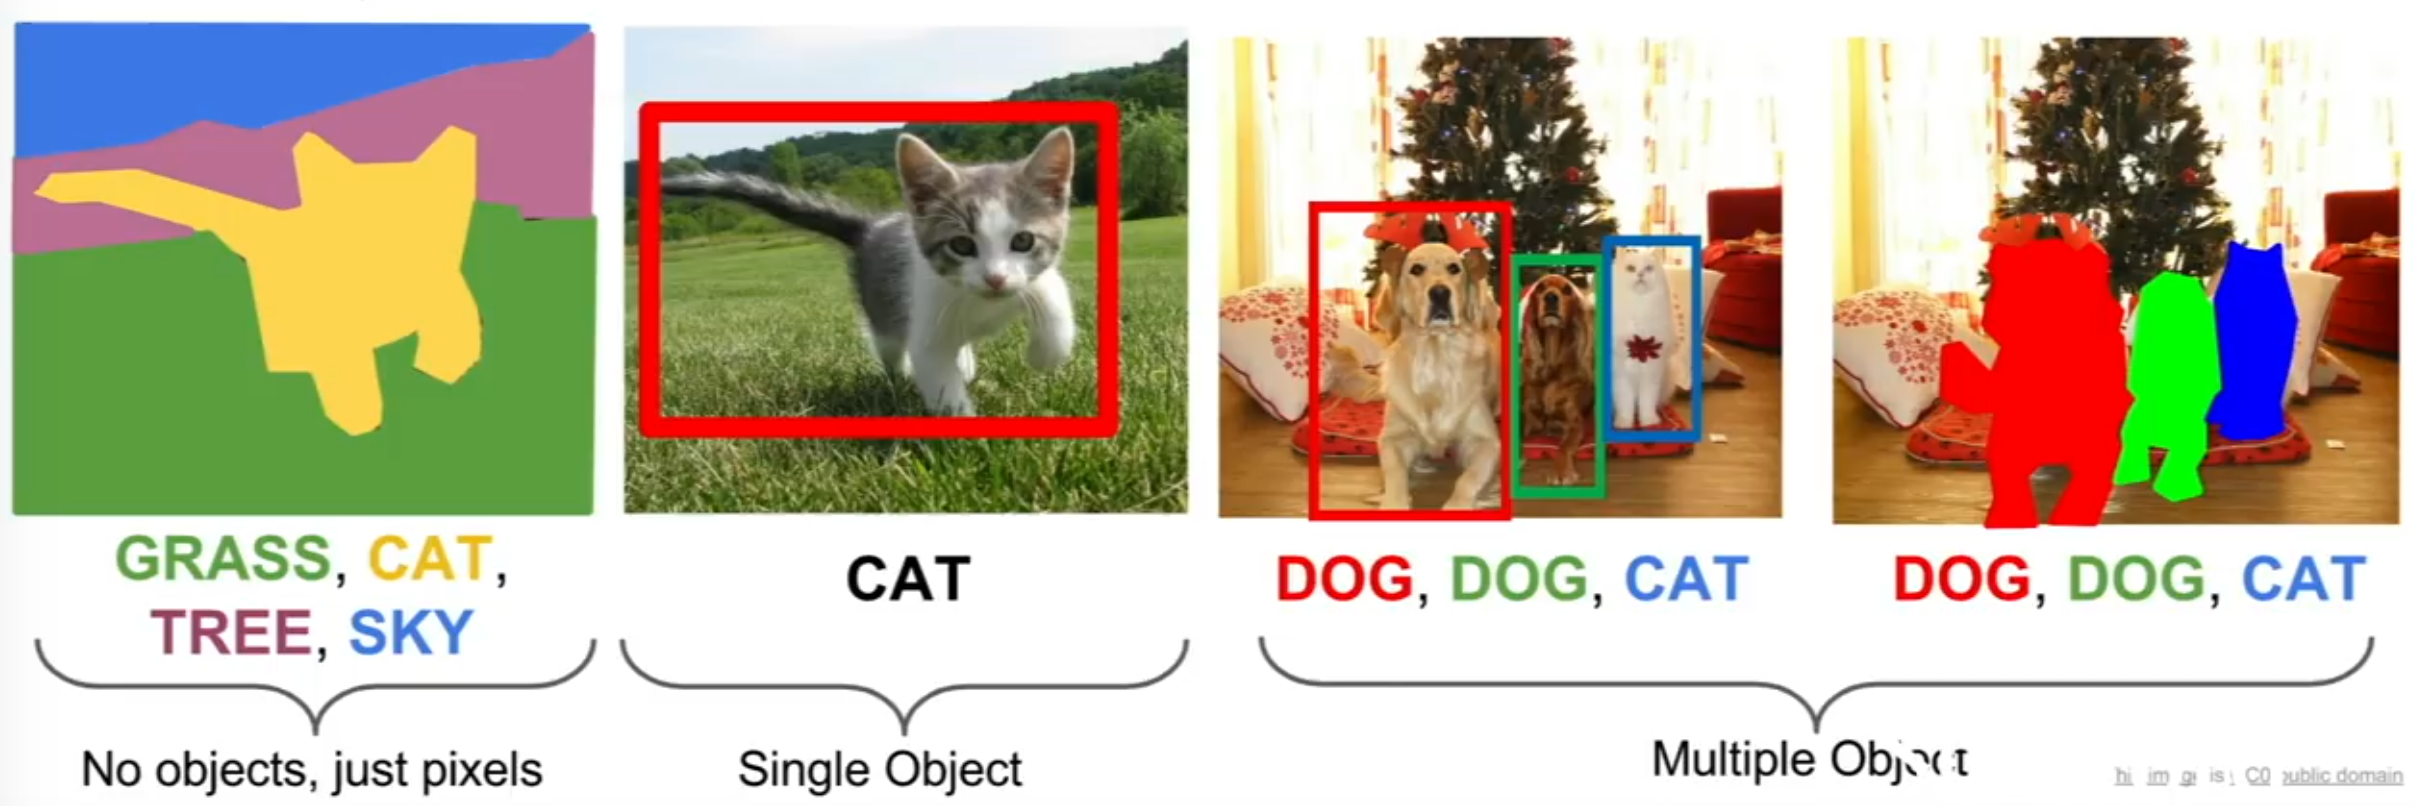
\includegraphics[width=0.5\columnwidth]{fei_fei_li/lecture_11/semantic_segmentation.png}

\subsection{Semantic Segmentation}

Decision for a category for every pixel in that image

Does not distinguish between instances of the object

\subsubsection{Bad Approaches to semantic segmentation}

\paragraph{Approach \#1 - Patch Based}

First idea - but a pretty bad one - patch based classification (sliding window)

extract a patch

classify center pixel with CNN

Computationally expensive and does not share computation for similar patches.

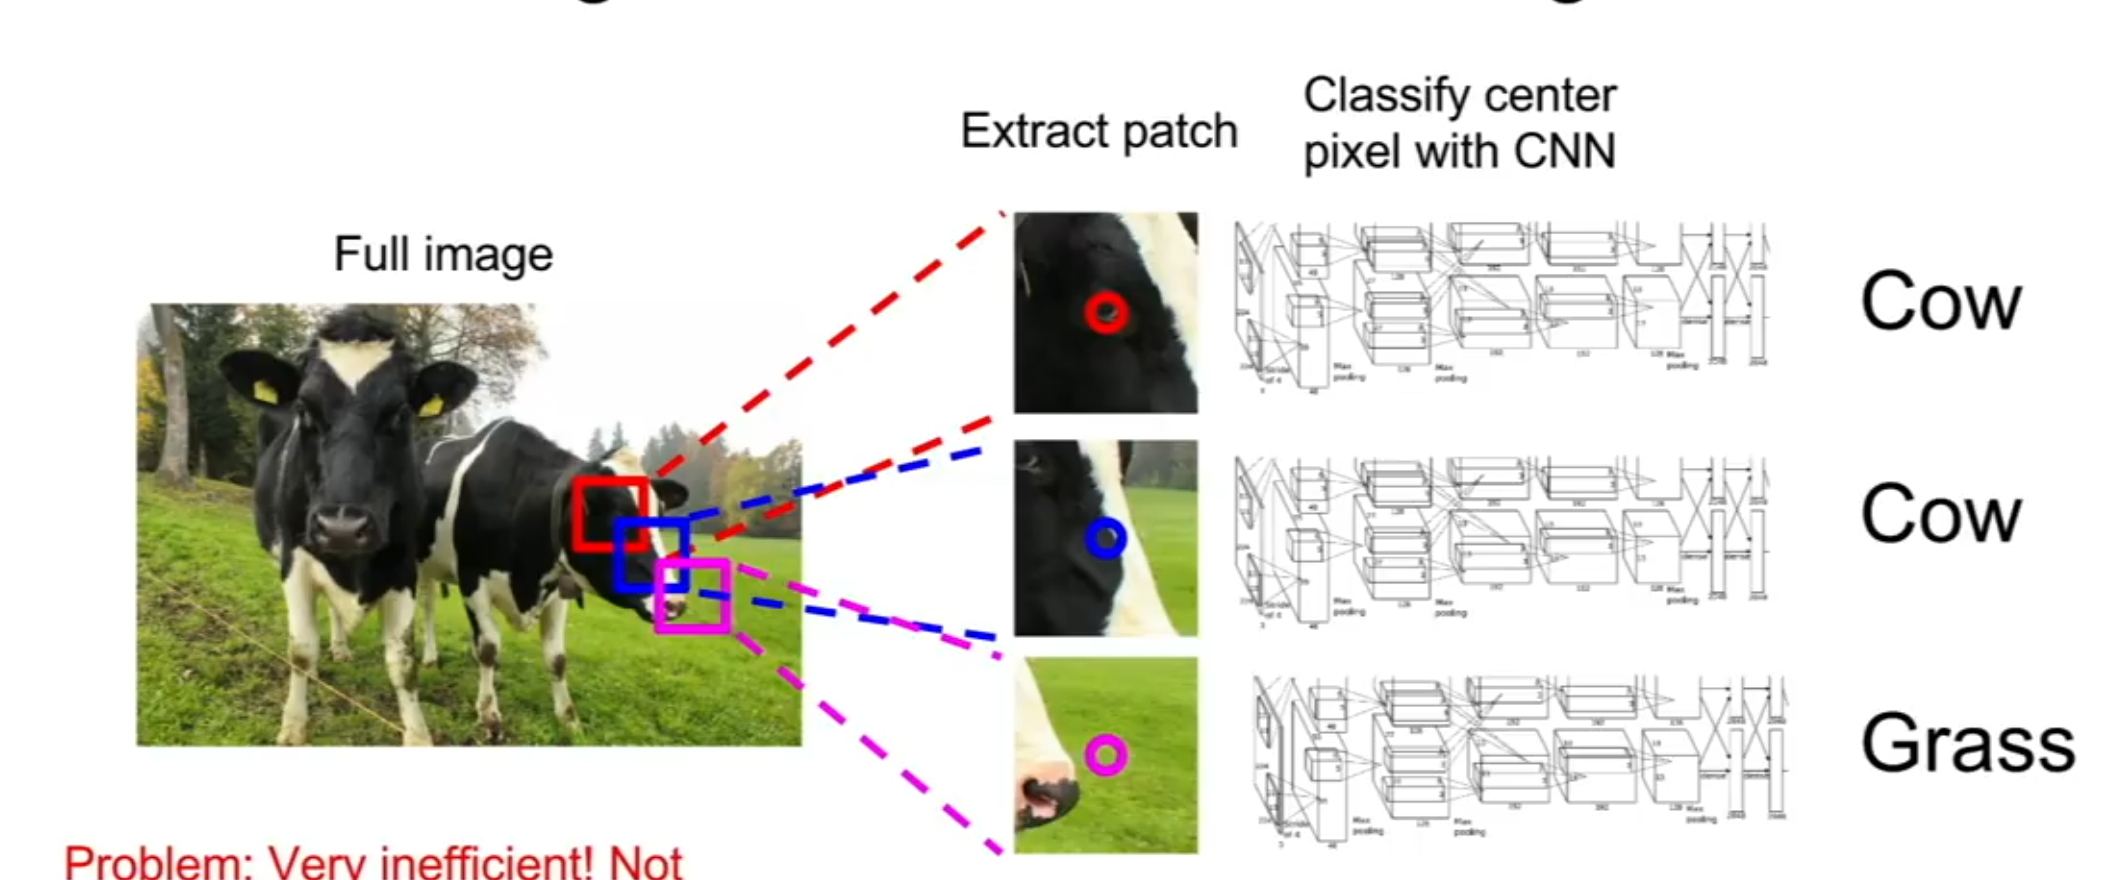
\includegraphics[width=0.5\columnwidth]{fei_fei_li/lecture_11/patch_based.png}

\paragraph{Approach \#2 - Fully convolutional}

Design a network as a bunch of conv layers

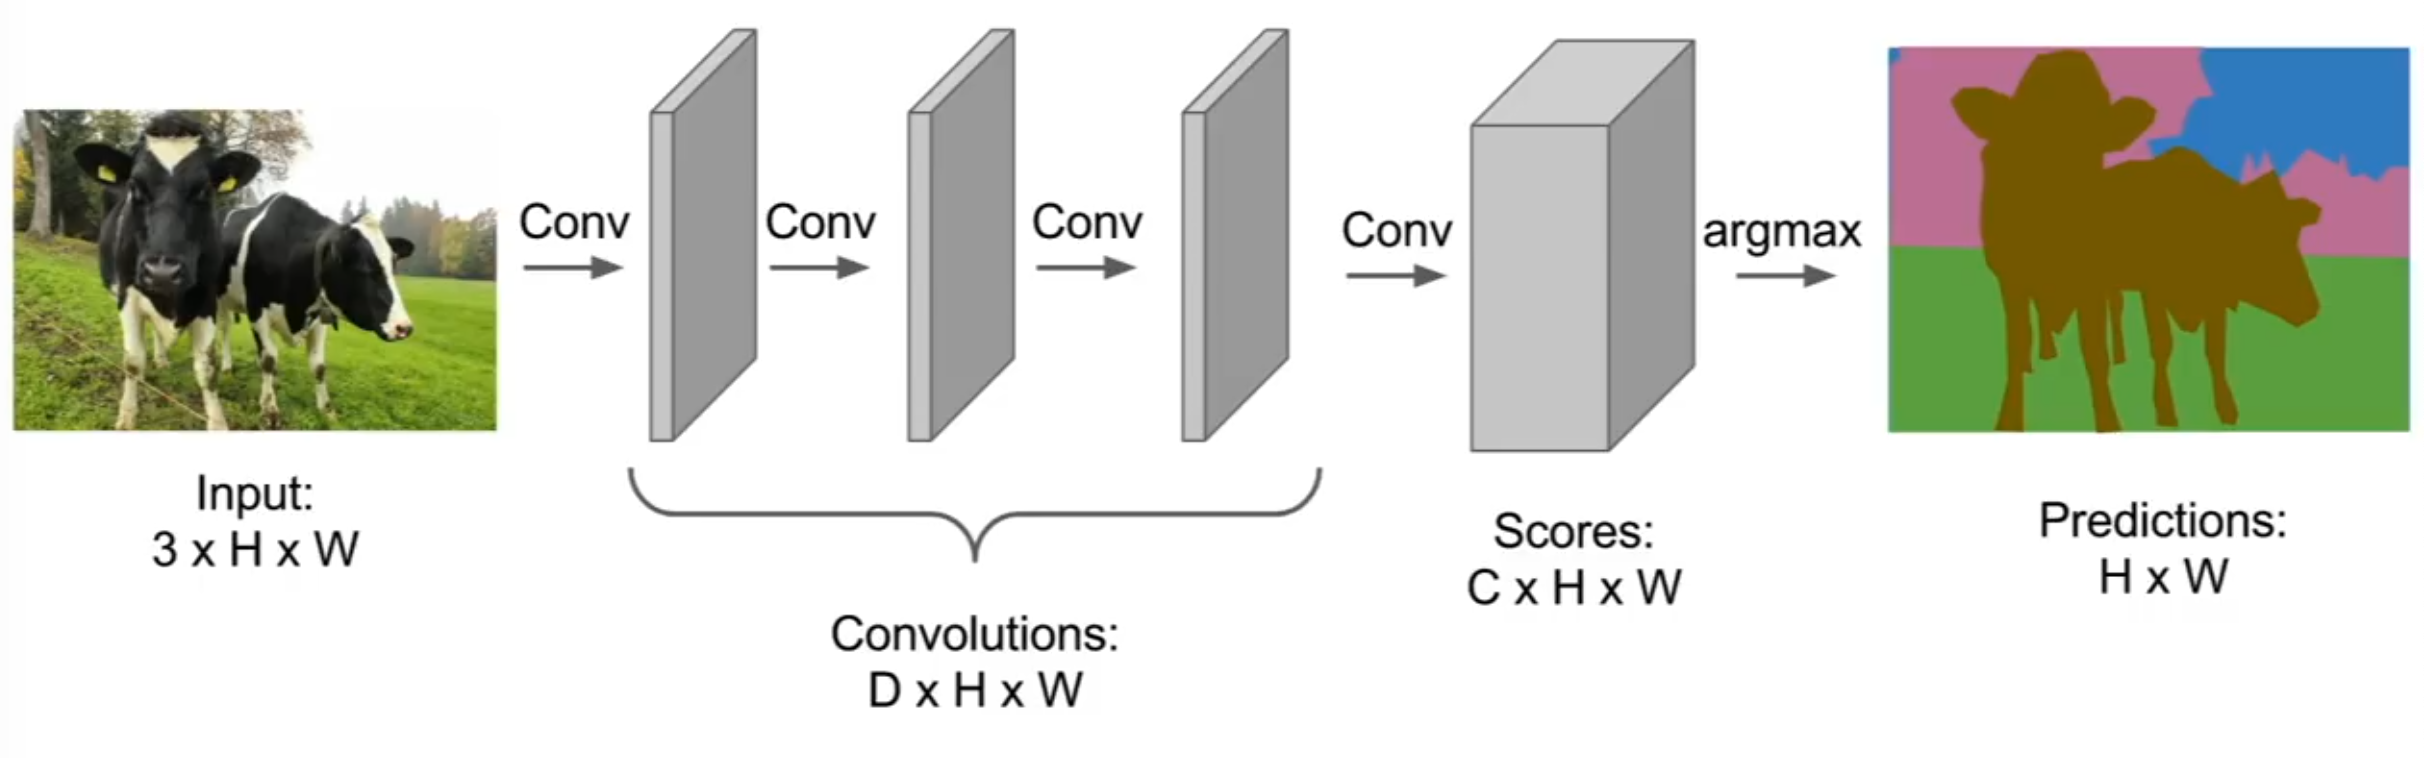
\includegraphics[width=0.5\columnwidth]{fei_fei_li/lecture_11/fully_convolutional.png}

- applying a bunch of conv that all have the same size of the image - very expensive!

\subsubsection{Approach \#3 - Down and upsampling}

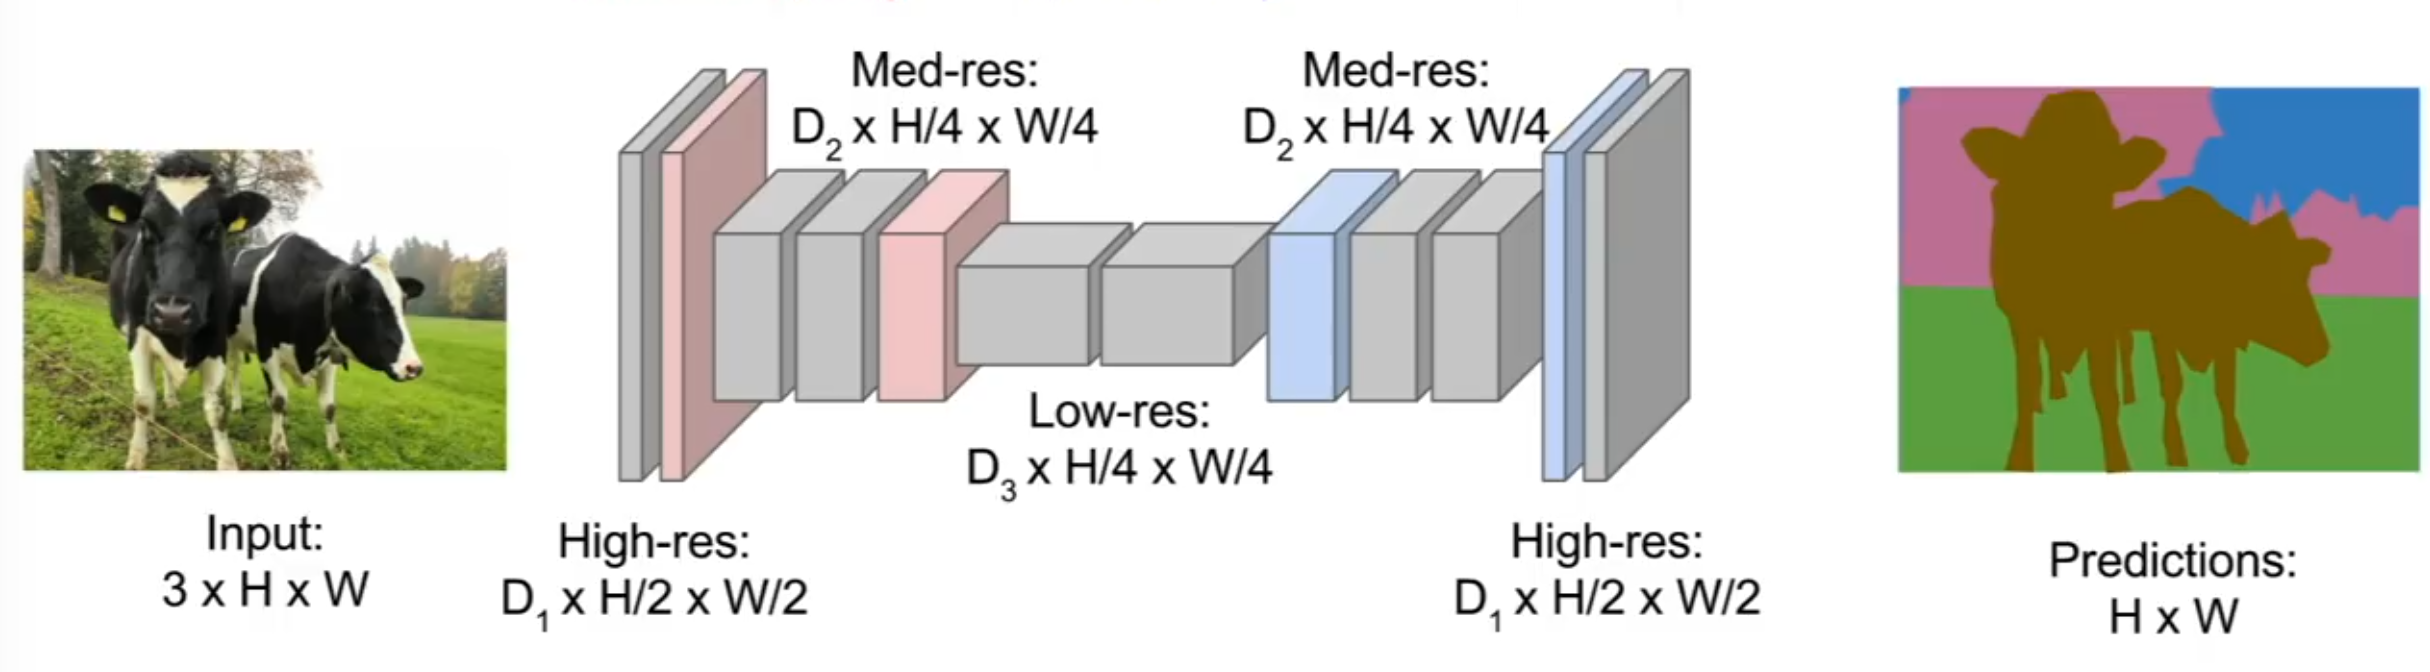
\includegraphics[width=0.5\columnwidth]{fei_fei_li/lecture_11/down_up_sampling.png}

In the second half of the network, the network will typically upsample the data

\paragraph{Unpooling}

Nearest Neighbor:

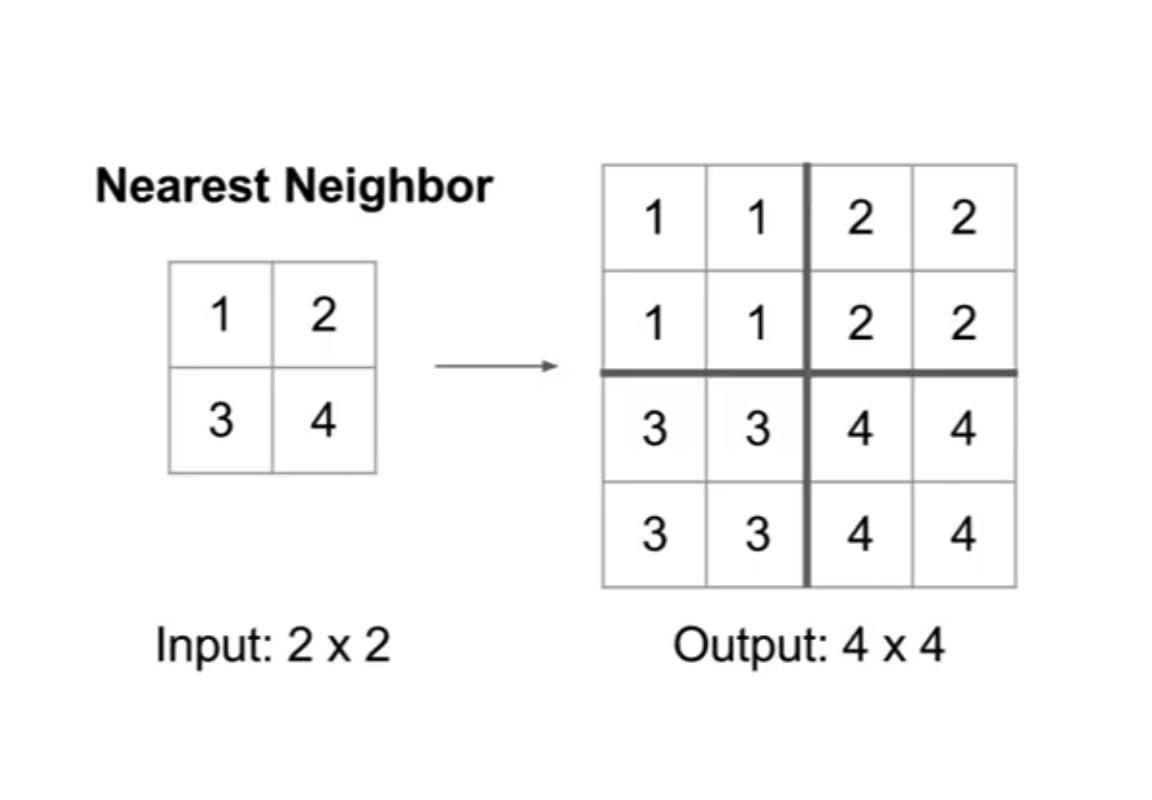
\includegraphics[width=0.5\columnwidth]{fei_fei_li/lecture_11/nn_uppooling.png}

Bed of nails:

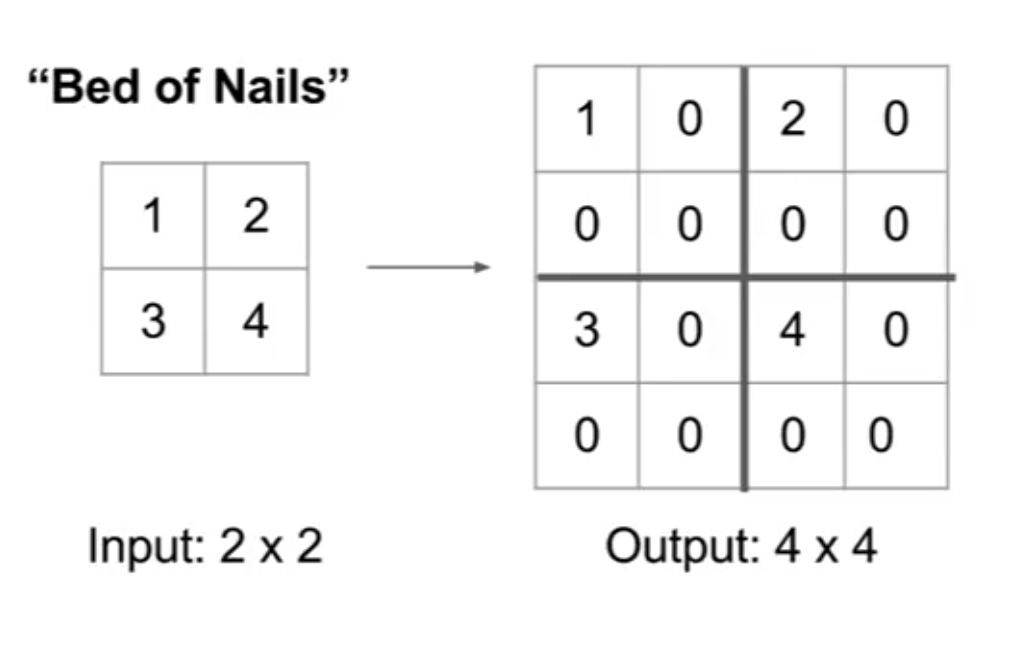
\includegraphics[width=0.5\columnwidth]{fei_fei_li/lecture_11/bed_of_nails.png}

Max Unpooling:

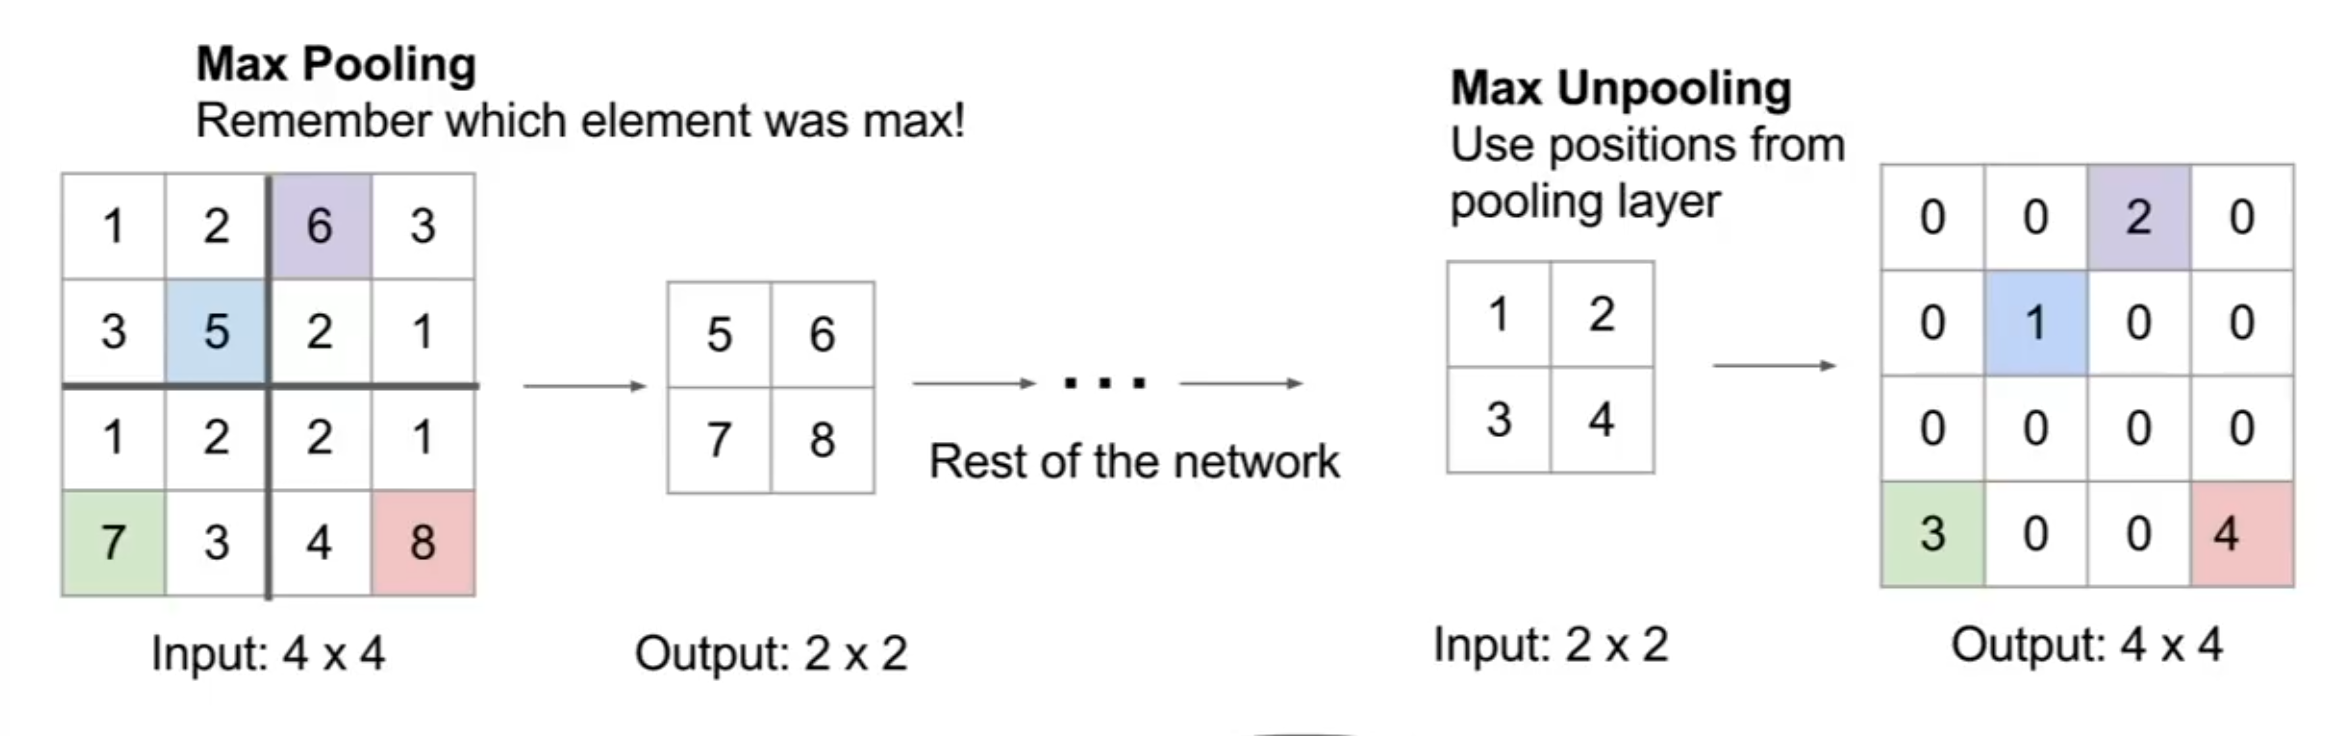
\includegraphics[width=0.5\columnwidth]{fei_fei_li/lecture_11/max_unpooling.png}

\subsubsection{Learnable Upsampling - Transpose Convolution }

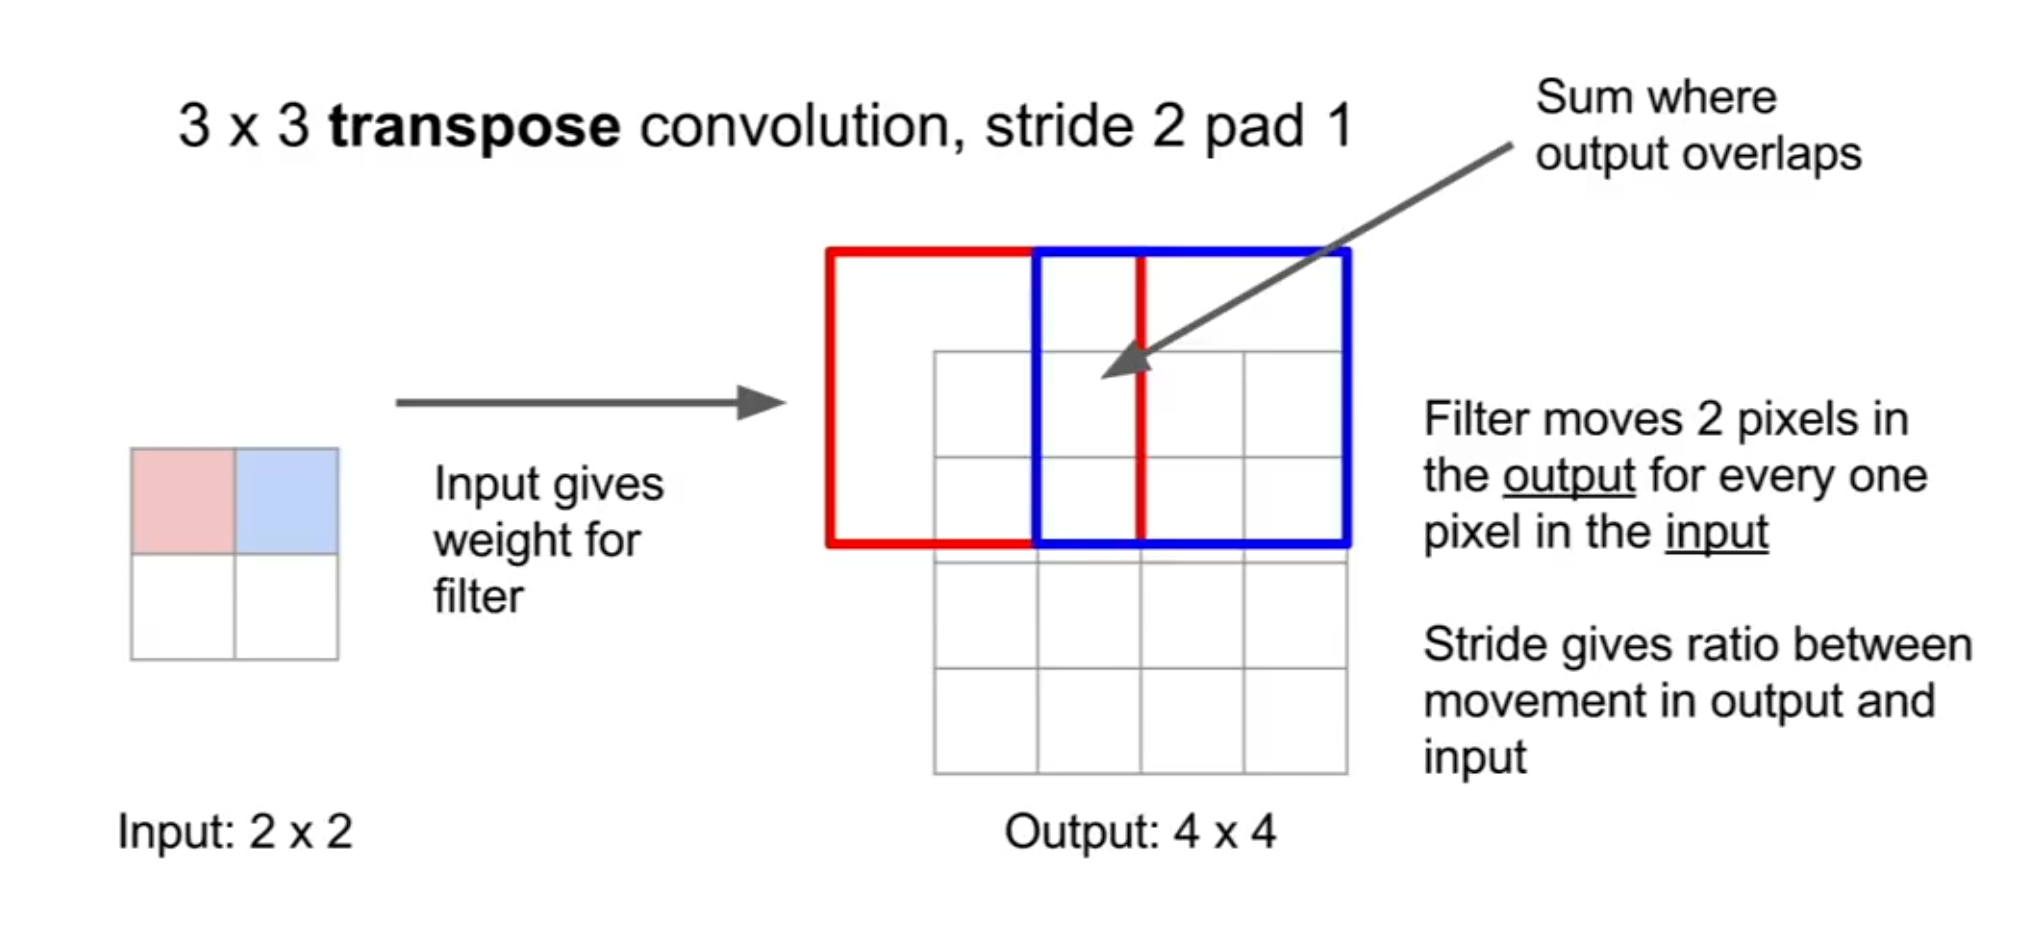
\includegraphics[width=0.5\columnwidth]{fei_fei_li/lecture_11/learnable_conv.png}

When the receptive fields in the output overlap, we sum

Sometimes called: 

- deconvolution

- upconvolution

- fractionally strided convolution 
- stride 1/2 convolution - if the stride is the relation between the input and output

- backward strided convolution

Convolution can be framed as matrix multiplication: $\vec x \star \vec a = X\vec a$

If we do a transpose to the $X$ matrix we get the "deconvolution" operation

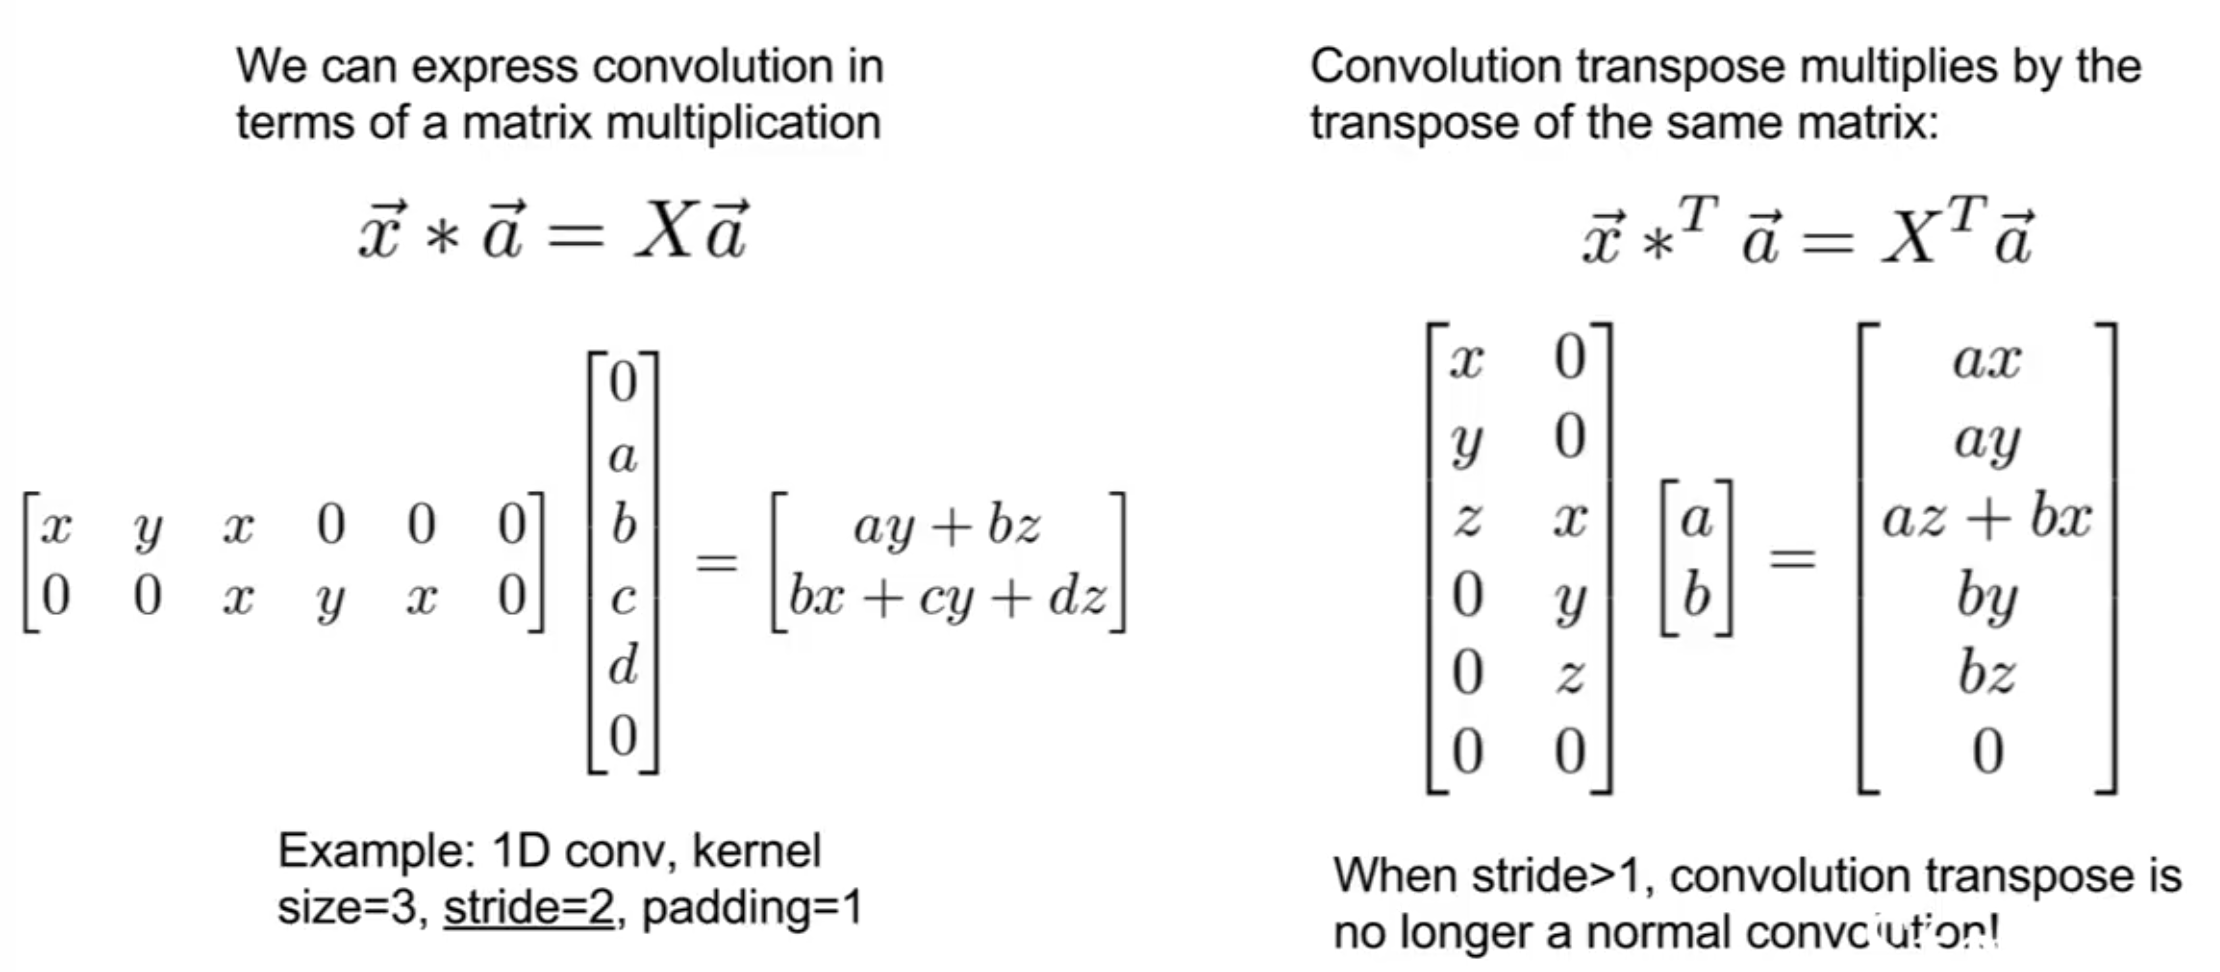
\includegraphics[width=0.5\columnwidth]{fei_fei_li/lecture_11/trans_conv_math.png}

\subsubsection{Classification + Localization}

i.e. bounding boxes

assumption: there is exactly one object in the image

can reuse previously familiar arch with one change: now there's a fully connected layer which also returns box coordinates

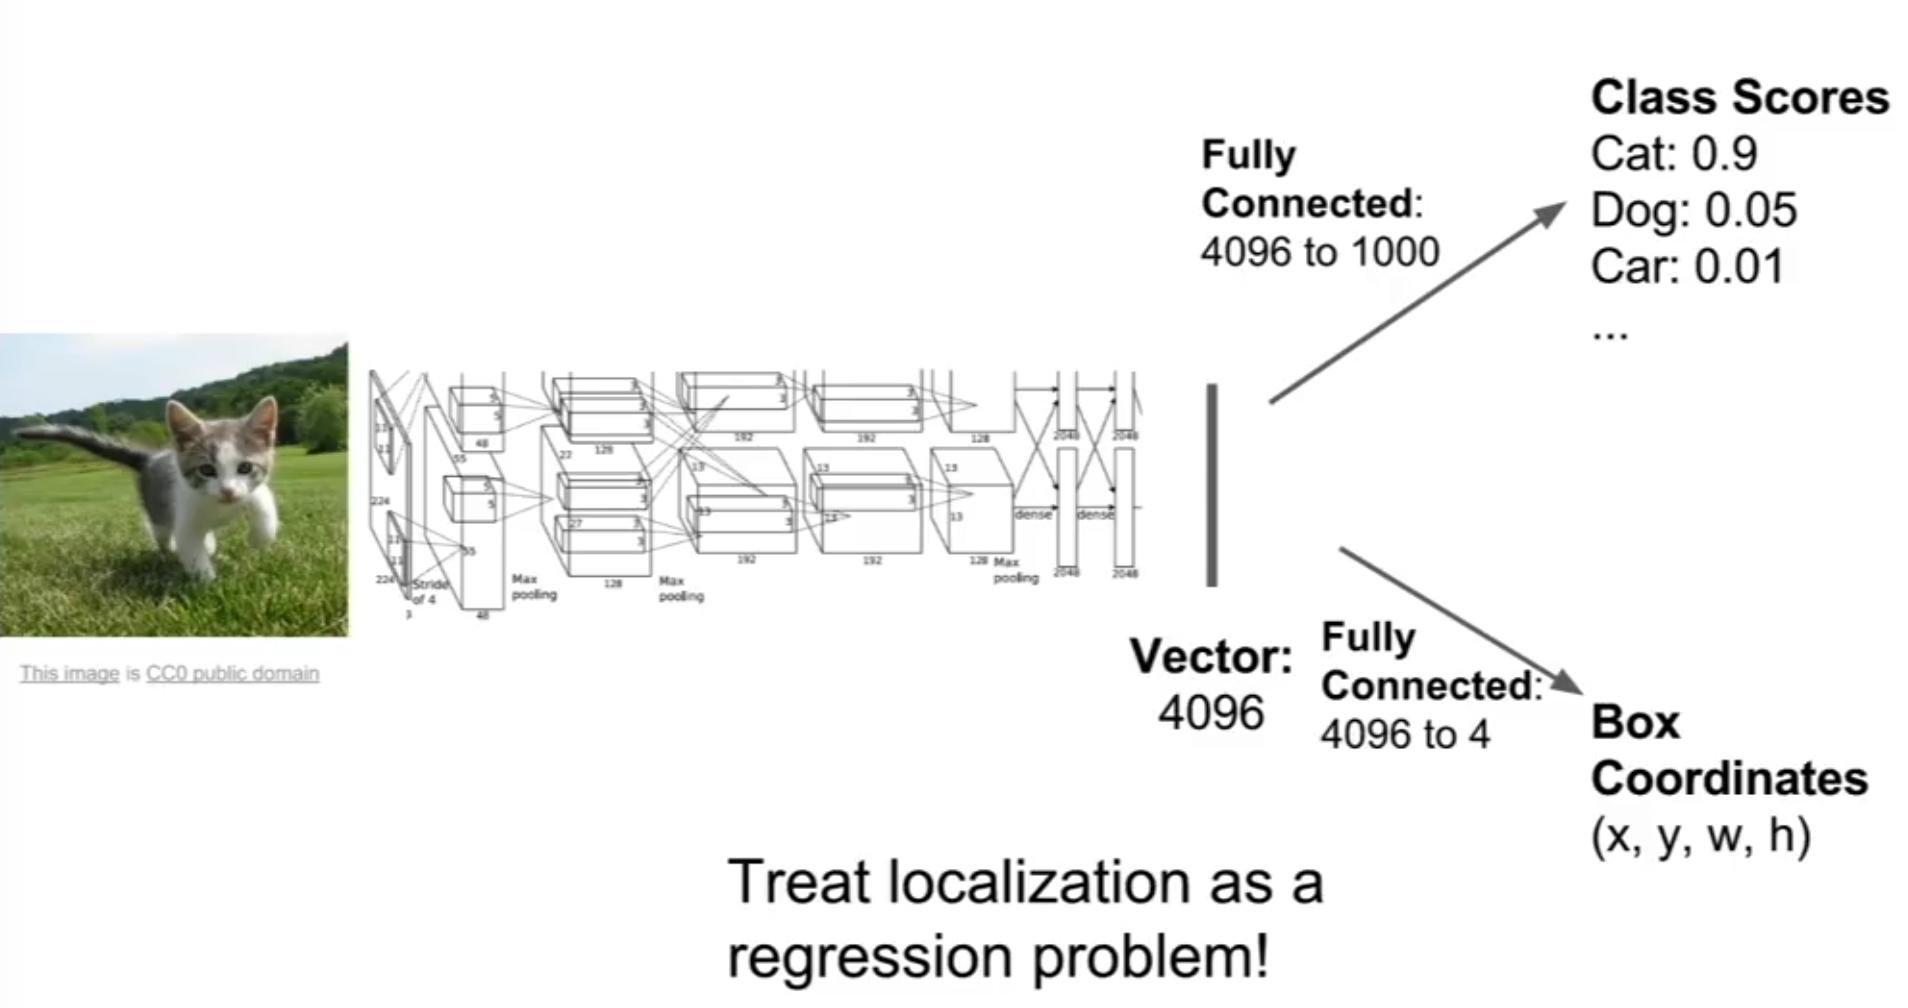
\includegraphics[width=0.5\columnwidth]{fei_fei_li/lecture_11/class_loc.png}

There are two loss functions:

softmax loss to create labels

L2 loss for the correct boss (simplest)

The assumption is that the images are labelled with these

The idea is that we have regression loss (what's that?)

multi task loss - have an additional hyperparamter that is used to scale both loss types, and take the gradient in respect to the weighted sum

the weighted hyperparamter changes the value of the loss function, which makes it harder to compute the gradient - cannot compare diff values for the hyperparamter directly as it directly affects the value of the loss

to deal with this: use some other metric of performance

better performance to train the network jointly

another possibility: freeze the network, train other parameters, and then fine tune the entire network

\paragraph{Human Pose Estimation}

Represent pose as a set of 14 joint positions

\subsubsection{Object Detection}

Different from localization - might have many number of outputs

\paragraph{Sliding window}

Different crops from the image - feed it through a classification network

We also add a category of background if it cannot find

Problem: how do you choose the crops? location, size, aspect ratio, etc.

\paragraph{Region Proposal Network}

Will generate boxes where objects may be present.

Relative fast to run - Selective Search

High recall, and also many regions without objects.

\subsubsection{R-CNN}

Put together all of the pipeline: 

Extract ROIs form proposal method

Warp ROIs to the fixed size for the downstream network

Run through CNN

Use SVM to compute grades (svm loss - hinge loss)

In addition, predict correction to the bounding box

Multi class loss, train the whole thing

Main problem: super slow on training and inference

\paragraph{Fast RCNN}

forward the whole image through convnet

create feature map of the image

roi pooling layer

fully connected layer

bounding box regressor

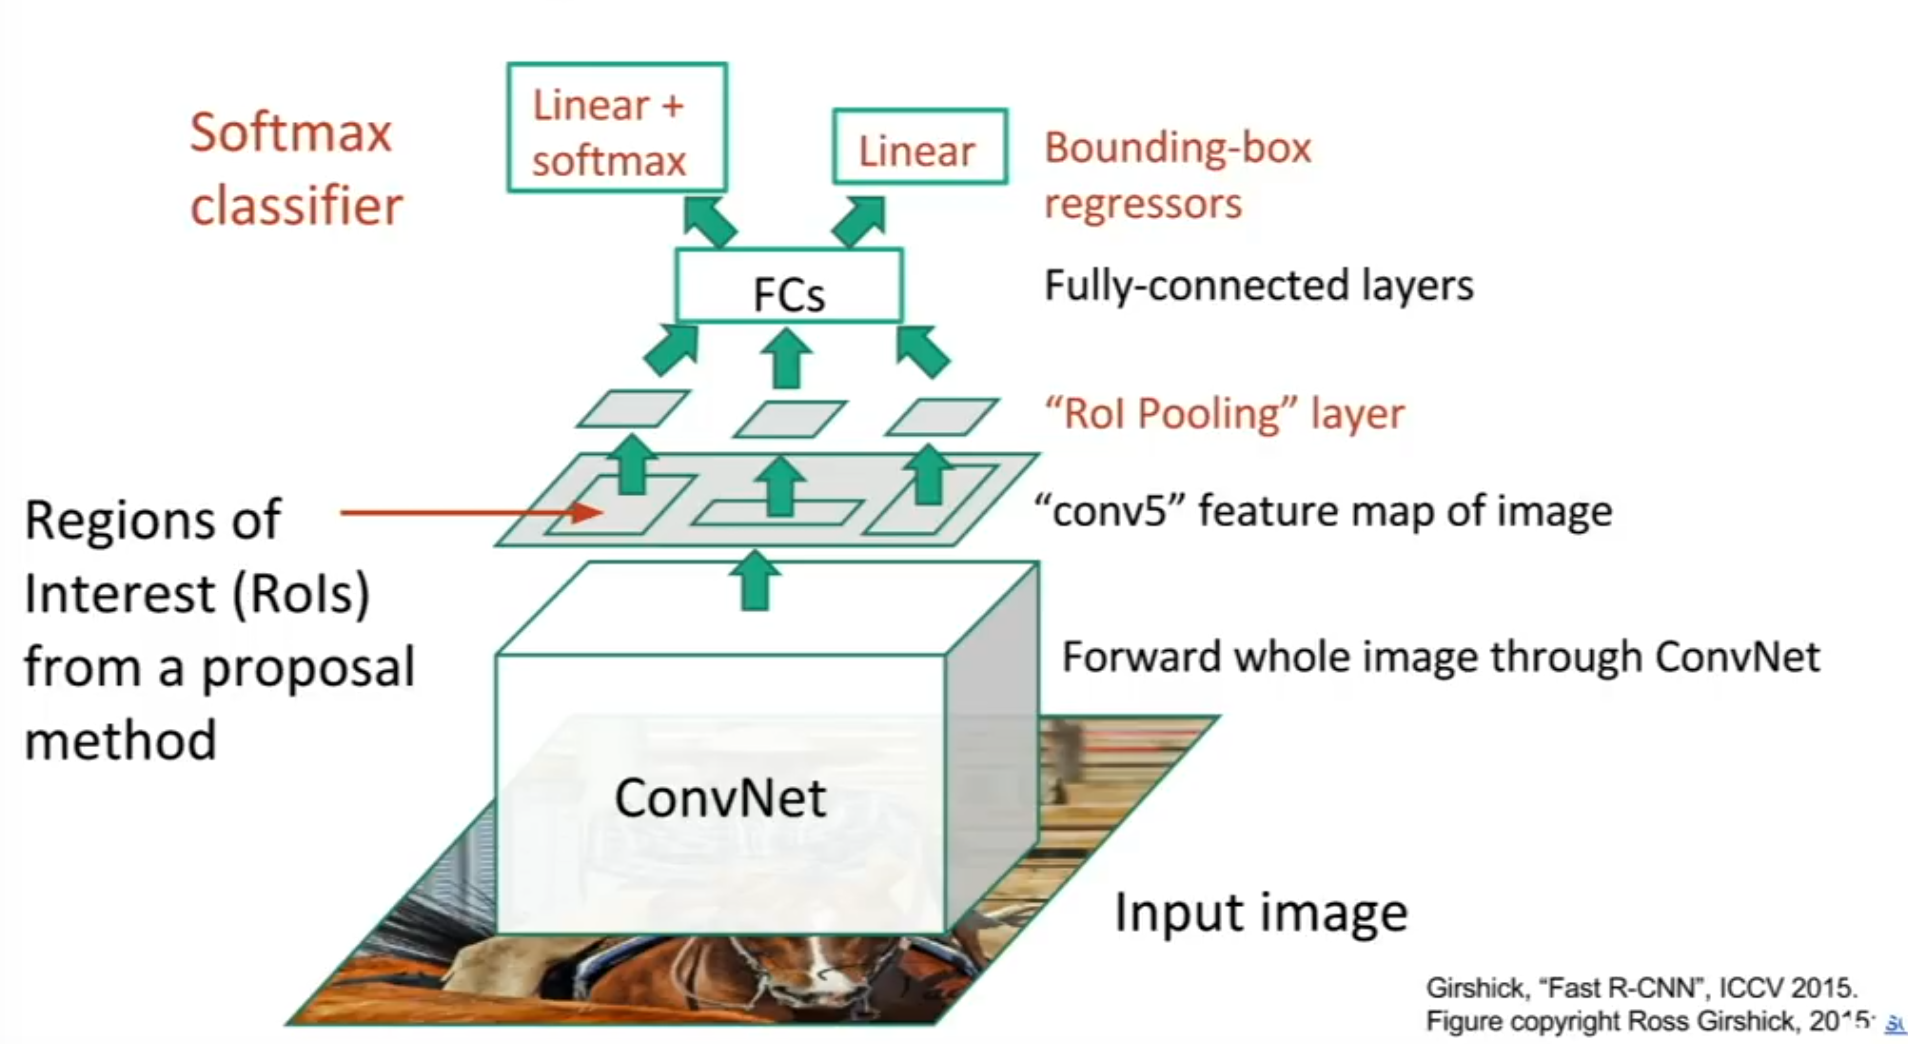
\includegraphics[width=0.5\columnwidth]{fei_fei_li/lecture_11/fast-rcnn.png}

During training add a multi class loss to do regression and do back prop:

\includegraphics[width=0.5\columnwidth]{fei_fei_li/lecture_11/fast_rcnn_2.png}

fast RCNN runtime is still dominated by the procedure to find ROIs.

\subsubsection{Faster RCNN}

Make the CNN do proposal 

Have to optimize for four! different tasks/ goals which might be tricky

Training ROI is tricky because there's no ground truth data - to do this, any overlap between ROIs and ground truth object is marked as positive and cases of no intersection are given a negative rating

Classification task - binary decision for each region

Removed the overhead from computing region proposals.

Once you're learning ROIs, you can bias the model to your data.

\subsubsection{Detection without Proposal}

The idea for both of this methods is to do object detection as a regression problem, and perform all of the tasks at once.

\includegraphics[width=0.5\columnwidth]{fei_fei_li/lecture_11/YOLO_SSD.png}

\paragraph{YOLO}

YOLO - you only look once

Feed forward single pass object detection.


\paragraph{SSD - Single Shot Detection}

\subsubsection{Instance Segmentation}

Predict the location and identities of the objects in the image

Rather than predict a bounding box, predict a segmentation mask for each of these objects.

\paragraph{Mask R-CNN }

Similar to Faster RCNN

Instance segmentation was trained on the Microsoft Coco dataset

\subsection{Visualization and Understanding}

\subsubsection{First Layer}

We can visualize each one of the filters directly:

We're visualizing the RGB layers from first layers of the filters. 

Observing  strong response to oriented edges in opposing colors

(this is from the pytorch model zoo)

\includegraphics[width=0.5\columnwidth]{fei_fei_li/lecture_12/first_layer_vis.png}

Visualizing higher level layers weights are less obvious - 16 channel input

16x20x7x7 filters?

\subsubsection{Last fully connected layers:}

\subsubsection{The last layer visualization}

4096d feature vector for an image

Nearest neighbors in feature space:  run all images through the network and collect the feature vectors

Can potentially be very different from in appearance, but similar in semantic content

There is nothing in the loss function that encourages these features end up close together.

\paragraph{Dimensionality Reduction}

Visualize the space of TC7 by reducing the dimensionality of the vectors from 4096 to 2 dimensions?

PCA

t-SNE

\paragraph{Maximally Activating Patches}

Keep track of what patches maximally activate neurons from a dataset and visualize them - gives an idea of what kind of features the neuron might be looking for.

\paragraph{Occlusion Experiments}

Check which parts of the image cause the largest change in the classification / probability / scores

\paragraph{Saliency Maps}

Visualize which pixels matter most for classification

Compute the gradient of (unnormalized) **class score** with respect to image pixels, take abs value and max over rgb channels.

This tells us how much the class score changes with the respect of each pixel

GrabCut + Saliency maps

\paragraph{Guided Back Propagation}

compute the gradient of neuron value with respect to image pixels

now in addition to the patches, we can see exactly which part of patch activates the neuron

\includegraphics[width=0.5\columnwidth]{fei_fei_li/lecture_12/patches.png}

\paragraph{Gradient Ascent}

Synthesize images that maximize the activation in the network.

Start with a neutral image, compute gradient with respect to the neuron you want to maximize, and update the image in that direction

For regularization: just regularize the $L_2$ norm of the image

Some people do stuff like 

- clipping pixel values

- gaussian blur image

This can be interpreted as projection of this max image onto a nicer image space

$\Rightarrow$ Visualizing this features and neurons would be a good exercises for me

Visualizing the higher level features shows that some of the class labels are multi modal

\subsubsection{Adversarial Examples}

Idea: 

1. start from an arbitrary image
2. pick arbitrary class
3. modify the image to maximize the class
4. repeat until network is fooled

\subsubsection{Feature Inversion}

Total variation - encourages absolute pixel differences between neighboring pixels - encourages spatial smoothness

\subsubsection{Natural Feature Synthesis}

~50 minutes into the lecture, i don't care about this

\paragraph{Texture Generation}

Nearest neighbor - simple approach that works pretty well for simple textures

March through the generated image and look at neighborhood around current pixel

But more complex texture do not work so well

Similar to gradient ascent in CNN

Gram Matrix -  

\subsubsection{Style Transfer}

\includegraphics[width=0.5\columnwidth]{fei_fei_li/lecture_12/text_synthesis.png}

The $C\times C$ matrix can be used as a feature descriptor, to describe which features tend to activate together the most.

The matrix throws away all spatial information because it averages all feature pairs in the image. 

Efficient to compute - 

$$ C \times H \times W \Rightarrow C \times HW \\$$ 

Using true covariance matrix also works but it is more expensive to compute

The gram matrix can be used to generate images with the same matrix:

\includegraphics[width=0.5\columnwidth]{fei_fei_li/lecture_12/texture_synthesis.png}

Using higher layers of features from the CNN results in larger features being reconstructed or transferred into the test image

\subsubsection{Style Transfer}

Feature matching + texture synthesis

Input: Content Image + Style Image

Minimize the feature reconstruction loss of content image and minimize texture loss on for texture image

\includegraphics[width=0.5\columnwidth]{fei_fei_li/lecture_12/style_transfer.png}

(might take a few hundred iterations to converge)

Can play with parameters - tradeoff between content and style

Resizing the style image gives control on the features which are going to be transferred

Problem: slow - many forward and backward passes.

Solution: train CNN to do the style transfer

Train (a few hours) - then single forward pass

Runs in real time

Fast style transfer - replaced batch normalization with instance normalization 

Google addressed this by training one network to do style transfer to many different styles

\section{Generative Models}

\subsection{Unsupervised Learning}

The strategy is: 

Data -> encoder -> features -> decoder -> reconstruction

The loss is trying to create a good reconstruction of the input data

Can be $L_2$ loss

Examples: 

Data: just data

Goal: learn the underlying hidden structure of the data

Examples: clustering, dim reduction, feature learning, density estimation

\paragraph{Density Estimation}

\includegraphics[width=0.5\columnwidth]{fei_fei_li/lecture_13/density.png}

In the unsupervised version, the data is cheap.



\subsection{Generative Models}

A class of models, where, given training data, the goal is to generate more examples from the same distribution.

Address density estimation 

- Explicit density estimation
- Implicit density estimation

Why?

- Realistic samples from artwork 

- Super-resolution

- Generative models of time-series data for simulation and planning

  - Good for reinforcement learning

- Learning latent variable representation

  \includegraphics[width=0.5\columnwidth]{fei_fei_li/lecture_13/taxonomy.png}

(for Ian Goodfellow tutorial on generative models)

\subsubsection{Pixel RNN + PixelCNN}

Fully visible belief networks:

Explicit density model

$p(x) = \Pi_{i=1}^n p(x_1 | x_1,\dots, x_{i-1})$ 

likelihood of the image $x$, the likelihood of each pixel given all previous pixel values

this is a complex transformation, we use NN 

Q: how to order the pixels?

\paragraph{PixelRNN}

Generate image pixels starting with one corner

Depending on previous pixels using a RNN with LSTM

Sequential generation - slow

\paragraph{PixelCNN}

Still generates an image from a corner

Use CNN to model the dependency over a context region

output: softmax loss at each pixel

$\Rightarrow$ i don't get it



\subsubsection{Autoencoders}

Input $(X)$ -> Encoder -> (Latent) Features (Z)

$dim(Z) < dim(X)$ - the features should capture the \emph{important} variation in the data

Encoders: linear, non linear, ReLU, 

Train the model as features that be used to reconstruct the original data

Decoder: usually same types of networks as the encoder.

\includegraphics[width=0.5\columnwidth]{fei_fei_li/lecture_13/encoder_decoder.png}

After this step, we don't need to decoder anymore - we can use this to initialize a supervised model:

\includegraphics[width=0.5\columnwidth]{fei_fei_li/lecture_13/supervised_encoder.png}

For example, this is used in cases where there is not a lot of data.

Autoencoders can reconstruct data and learn new features to initialize a supervised model. 

The features capture the variation in the training data. Now how can we use them to generate new data?

\subsubsection{Variational Autoencoders}

Probabilistic spin on autoencoders - will let us sample from the model to generate data.

Assuming training data $\{x^{i}\}_{i=1}^N $ is generated  from underlying, unobservred latent representation $z$ 

Generation process: sample from a prior over $z : p_{\theta^\star}(z)$  usually a Gaussian 

Now sample from true conditional: $p_{\theta^\star}(x|z^i)$ \includegraphics[width=0.5\columnwidth]{fei_fei_li/lecture_13/decoder_training.png}

Want to estimate the true parameters $\theta^\star$ so we can generate new data.

Gaussian assumption is reasonable for latent attributes such as pose, expression etc.

The conditional representation $p(x|z)$ is much more complex and it is represented through a network (decoder neural network)

How to train this model?

From Fully Visible Belief Networks: learn  model parameters to maximize the likelihood of training data:

$p_\theta(x) = \int p_\theta 	(z) p_\theta(x|z)dz$ 

This integral is intractable - it is impossible to integrate over all z

Posterior density is also intractable: $$p_\theta(z|x)=p_\theta(z)/p_\theta(x) $$

The solution is to define another encoder network $q_\theta(z|x)$ that approximates $p_\theta(z|x)$. This allow us to derive a lower bound on the data likelihood which is tractable. 

The encoder network will give out the mean and covariance of $z|x$:

\includegraphics[width=0.5\columnwidth]{fei_fei_li/lecture_13/encoder_theta.png}

and similarly we have a probabilistic decoder network:

\includegraphics[width=0.5\columnwidth]{fei_fei_li/lecture_13/prob_decoder.png}

Both of these network produce distributions, we can sample from them $x|z$ and $z|x$ .

These network types are also known as recognition and inference and generation networks

\subsubsection{Recap:}

- PixelCNNs define tractable density function, optimize the likelihood of training data

- VAE define intractable density function with latent $z$, - but cannot be optimized directly, instead derive and optimize lower bound on the prob. dist.
- GANs - give up on explicitly modeling density, just want to sample

\subsubsection{Generative Adversarial Networks}

Want to sample from a complex, high dimensional training distribution.

To actually do this, we sample from a simple distribution (random noise) and use a network that learned a transformation from this to the training distribution.

\includegraphics[width=0.5\columnwidth]{fei_fei_li/lecture_13/gans_1.png}



To learn this transformation network is to look at this as two player game:

Generator Network: try to fool the discriminator by generating real looking images.

Discriminator network: try to distinguish between real and fake images.

\includegraphics[width=0.5\columnwidth]{fei_fei_li/lecture_13/gan_pipeline.png}

Both networks are jointly trained as a minimax game:

$$ \min_{\theta_g} \max_{\theta_d} \left[ \mathbb{E}_{x\sim p_{data}}\log D_{\theta_d}(x)+\mathbb{E}_{z\sim p(z)}\log(1-D_{\theta_d}(G_{\theta_g}(z))) \right]$$

The discriminator outputs likelihood in  $(0,1)$ of real images

The first term is the disc output for real data $x$ drawn from $p_{data}$

The second D term is the discriminator output for generated fake data.

The discriminator $\theta_D$ wants to maximize this objective - $D(x)$ is close to 1 $D(G(z))$ is close to 0 (fake data)

The generator $\theta_z$  wants to minimize the objective s.t. $D(G(z))$ is as close to 1

The optimization to do this goes as follows: 

1. Gradient ascent on the discriminator

   $$ \max_{\theta_d} \left[ \mathbb{E}_{x\sim p_{data}}\log D_{\theta_d}(x)+\mathbb{E}_{z\sim p(z)}\log(1-D_{\theta_d}(G_{\theta_g}(z))) \right]$$

2. Gradient descent on the generator:

   $\min_{\theta_g} \left[ \mathbb{E}_{z\sim p(z)}\log(1-D_{\theta_d}(G_{\theta_g}(z))) \right]$

In practice this does not work very well:

\includegraphics[width=0.5\columnwidth]{fei_fei_li/lecture_13/gan_loss.png}

The gradient is weak when the generator has not learned how to generate good samples yet. So instead we maximize the likelihood that the discriminator is wrong using a different objective:

$\max_{\theta_g} \mathbb{E}_{z\sim p(z)}\log(D_{\theta_d}(G_{\theta_g}(z)))  $

\includegraphics[width=0.5\columnwidth]{fei_fei_li/lecture_13/gan_fixed_loss.png}

Jointly training these two networks is challenging, unstable, etc.

Choosing objective with better loss landscapes helps training.

\includegraphics[width=0.5\columnwidth]{fei_fei_li/lecture_13/full_opt_pipeline.png}

The lecture also shows how the vectors of the params these networks generate are interpretable, for examples mean smiling women - mean neutral women + mean neutral man -> smiling man

\includegraphics[width=0.5\columnwidth]{fei_fei_li/lecture_13/interpetable.png}

Radford et al. ICLR 2016

\includegraphics[width=0.5\columnwidth]{fei_fei_li/lecture_13/year_of_gan.png}



https://github.com/soumith/ganhacks

GAN Summary:

pro: state of the art samples

cons: tricky to train, can't solve inference

\section{Reinforcement Learning }

\subsection{Markov Decision Process}

Markov property: current state completely characterized the state of the world

Define by: $(\mathcal{S,A,R},\mathbb{P},\gamma)$

$\mathcal{S}$ set of possible states

$\mathcal{A}$ set of possible actions

$\mathcal{R}$ set of possible rewards given state, action pair 

$\mathbb{P}$ transition probability

$\gamma$ discount factor

\section{Adversarial Examples}

Adv example - all ML models are vulnerable. 

Initially it was assumed that adv. examples were due to overfitting

Something important he said: adv. examples might be closer to underfitting than overfitting. For example, generating a adv example and adding the same diff vector to many objects will cause to miss-labelling of any example they're added to.

After this observation, the hypothesis changed to underfitting, or the model being too linear

Example:

\includegraphics[width=0.5\columnwidth]{"fei_fei_li/lecture_16/Screenshot 2019-10-25 at 16.16.26.png"}

Another interesting observation about this example - both corners are labelled as very green/blue although we have not seen any examples in these regions -> very high confidence very far from decision boundary

\includegraphics[width=0.5\columnwidth]{"fei_fei_li/lecture_16/Screenshot 2019-10-25 at 16.18.19.png"}

LSTM is doing addition operation which is also linear. 

Linearity: the mapping between the input of the model to the output of the model.

The mapping from the parameters of the network to the output are highly non linear (this is why training is difficult)

This means it is a lot easier to manipulate and optimize the input the model vs. the model


